\documentclass[12pt, a4paper,oneside]{book}
% Подключение библиотеки
\usepackage{/Users/vladbelousov/Desktop/Semestr_4-FP-NSU/Настройка/library}

\makeatletter
\@addtoreset{corollarycounter}{section}
\@addtoreset{theorem}{section}
\@addtoreset{definition}{section}
\@addtoreset{lemma}{section}
\@addtoreset{proposition}{section}
\makeatother  

\begin{document}

\begin{titlepage}
    \thispagestyle{empty}  % Отключаем нумерацию страницы на титульном листе
    \centering
    \vspace*{1cm}  % Отступ сверху

    \textbf{\huge Конспект лекций по дисциплине}  \\[1.5cm]  % Название
    \textbf{\Huge Дифференциальные уравнения}  \\[2cm]   % Название дисциплины (оставьте пустым для добавления вручную)
    \textbf{\Large Новосибирский государственный университет} \\[0.5cm]
    \textbf{\large Физический факультет} \\[0.5cm]
    \textbf{\large 4-й семестр} \\[0.5cm]
    \textbf{\large 2025 год} \\[10cm]

    \begin{flushright}
        \large Студент: Б.В.О \\[0.5cm]  % Ваше имя
        Преподаватель: Скворцова Мария Александровна  % Ф.И.О. преподавателя
    \end{flushright}
\end{titlepage}

\tableofcontents  % Создание оглавления

\def\mainfile{}  % Определяем макрос для основного файла
%Февраль
% Условная компиляция для самостоятельной работы
\ifdefined\mainfile
    % Если это часть основного файла, не добавляем начало и конец документа
\else
    \documentclass[12pt, a4paper]{report}
    \usepackage{/Users/vladbelousov/Desktop/Semestr_4-FP-NSU/Настройка/library}
    \usepackage[utf8]{inputenc} % Подключение поддержки UTF-8
    \begin{document}
\fi

%%-------------------------------%%

\chapter{Вариационное исчисление.}

\section{Примеры задач вариационного исчисления}

\textit{Задача математического анализа: } 



Есть кривая заданная функцией \( f(x) \) найти точки экстремума: 

\[  f'(x)=0 \Rightarrow {x_1,x_2}-{\text{точки, подозреваемые на экстремум}  }   \] 
\begin{gather*}
    f''(x_1)<0 \Rightarrow x_1  - \max  \\
    f''(x_2)>0 \Rightarrow x_2 - \min    
\end{gather*}

\textit{Задача вариационного исчисления:} 

Функционал: \( I [y]= \int_{x_0}^{x_1}F(x,y(x),y'(x))dx  \) 

Найти функцию \( y(x) \) такую, что \( I[y] \) принимает \( \min  \) или \( \max  \) 

\begin{flushleft}
    Пример 1 : задача наискорейшего спуска (задача Брахистохроне)
\end{flushleft}

Найти кривую \( y(x) \)  по которой тело из точки А в точку В попадет за наименьшее время. 

\begin{center}
    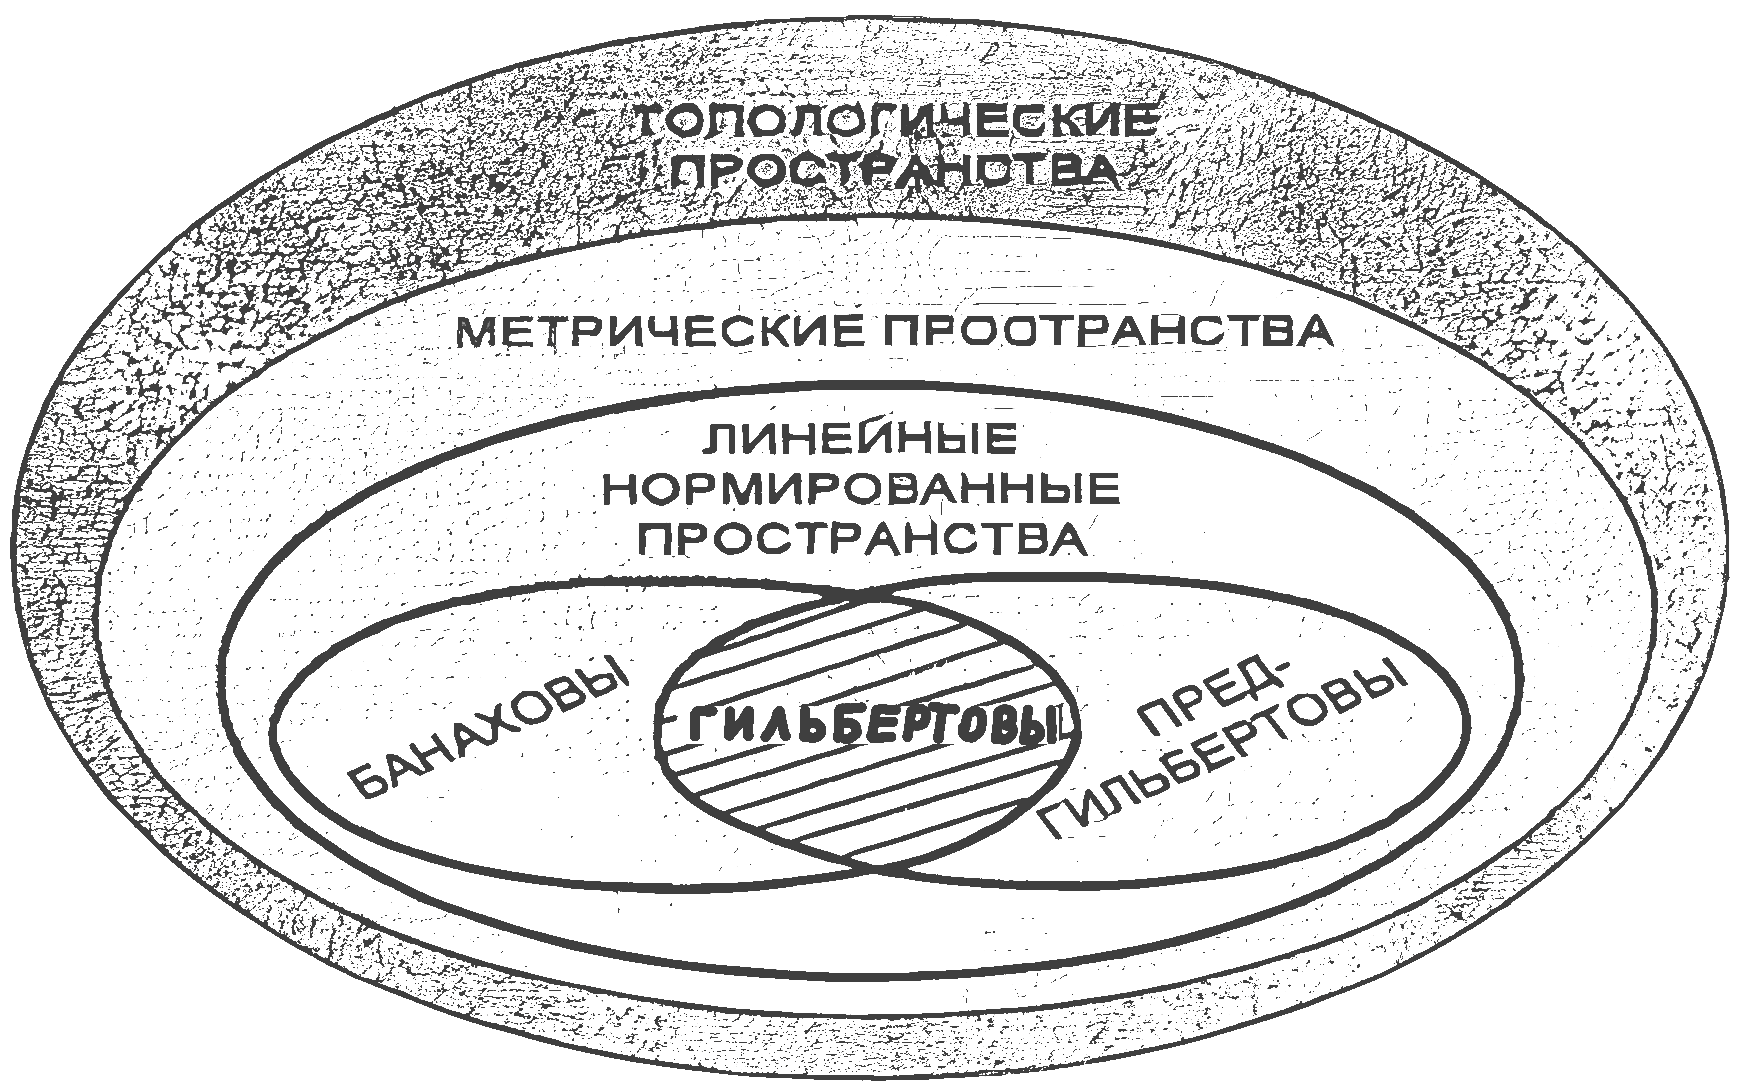
\includegraphics[width=0.5\textwidth]{/Users/vladbelousov/Desktop/Semestr_4-FP-NSU/ДфУ/Лекции_по_дням/image/1.png}
\end{center}

\begin{gather*}
   \text{З.С.Э: }  mgy_0+0= mgy(x)+ \frac{m |v| ^2}{2} \\
    \lvert v  \rvert =\sqrt{v_x ^2 + v_y ^2} = \sqrt{\left( \frac{\partial x}{\partial t}  \right) ^2 +\left( \frac{\partial y }{\partial t}  \right) ^2 }= \sqrt{1+(y'(x))^2} \frac{dx}{dt} \\
    \sqrt{2g(y_0- y(x)) }= |v|= \sqrt{1+(y(x)')^2} \frac{dx}{dt} \\
    T= \int_{0}^{T}dt= \int_{x_0 }^{x_1} \frac{\sqrt{1+(y'(x))^2}}{\sqrt{2g(y_0+ y(x)) }} dx   
\end{gather*}

\begin{flushleft}
    Пример 2 : задача поверхности вращения наименьшей площади. 
\end{flushleft}

\begin{center}
    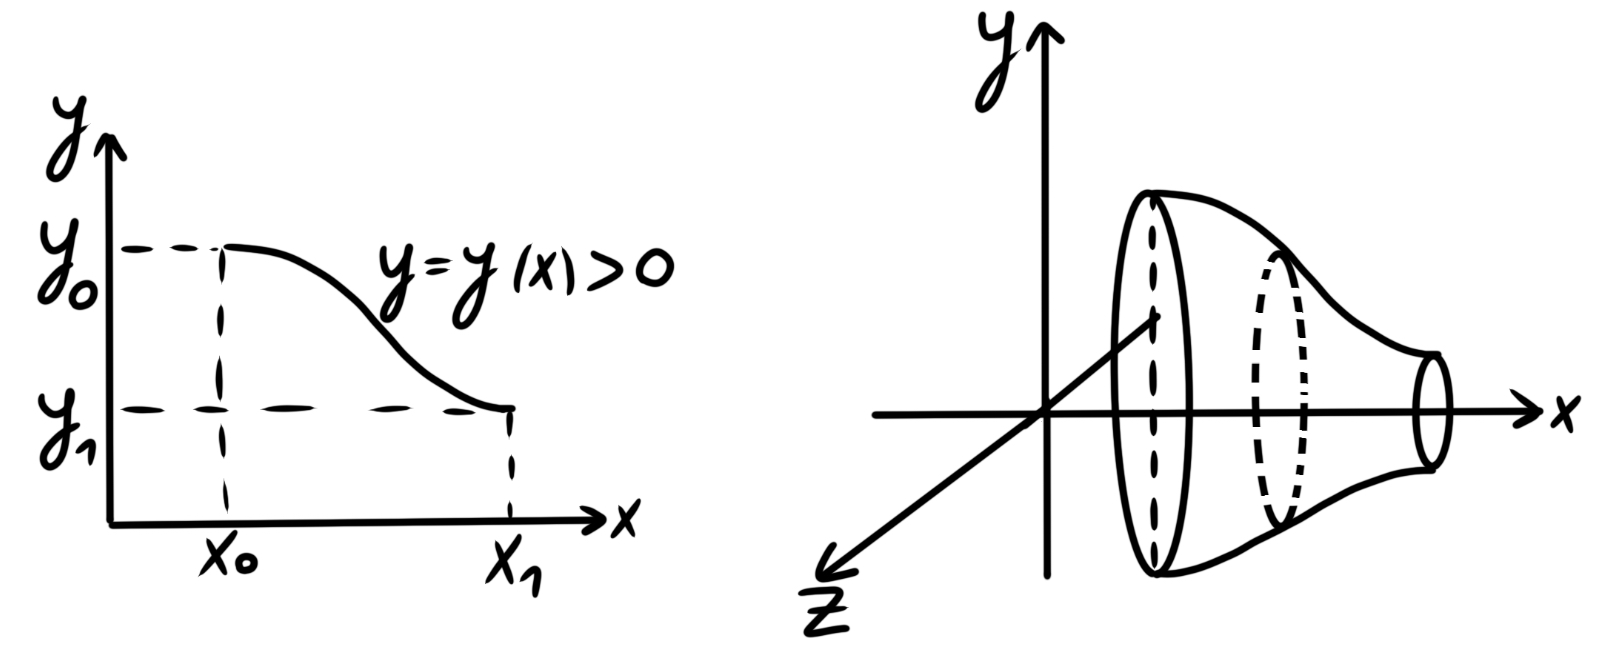
\includegraphics[width=0.8\textwidth]{/Users/vladbelousov/Desktop/Semestr_4-FP-NSU/ДфУ/Лекции_по_дням/image/2.png}
\end{center}

Площадь \( S \to \min  \) 

\begin{center}
    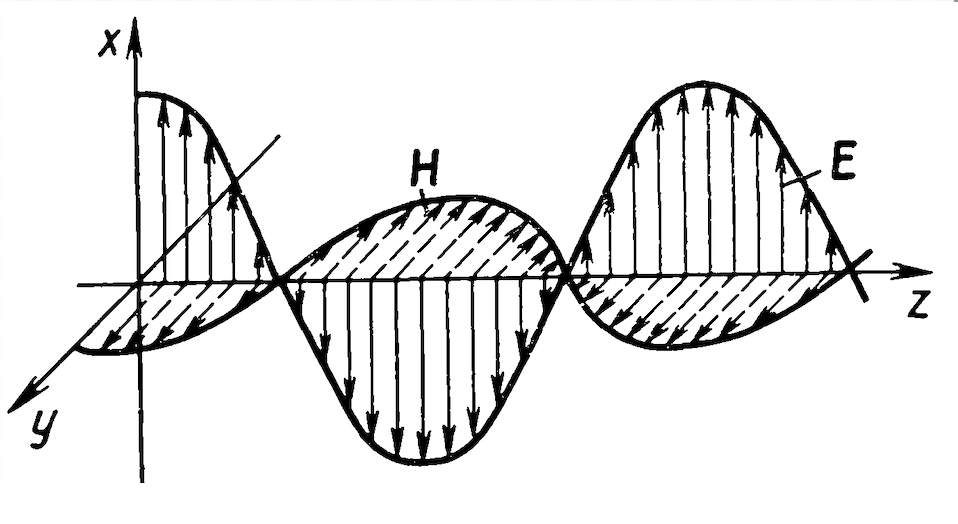
\includegraphics[width=0.5\textwidth]{/Users/vladbelousov/Desktop/Semestr_4-FP-NSU/ДфУ/Лекции_по_дням/image/3.png}
\end{center}

\begin{gather*}
    \Delta \delta= \sqrt{(\Delta x ) ^2 + ( \Delta y) ^2} = \sqrt{1 + \left( \frac{\Delta y}{\Delta x}  \right) ^2} \Delta x \\
    \Delta S = 2 \pi y (x) \Delta \delta \\
    \sum  \Delta S \xrightarrow{\Delta x \to  0}  \int_{x_1}^{x_2} 2 \pi y(x ) \sqrt{1+(y'(x))^2}dx  
\end{gather*}


\begin{flushleft}
    Пример 3 : задача о геодезических на поверхности.
\end{flushleft}

Найти кривую, проходящую через точки А и В, лежащую на поверхности, которая имеет наименьшую длину.

\begin{center}
    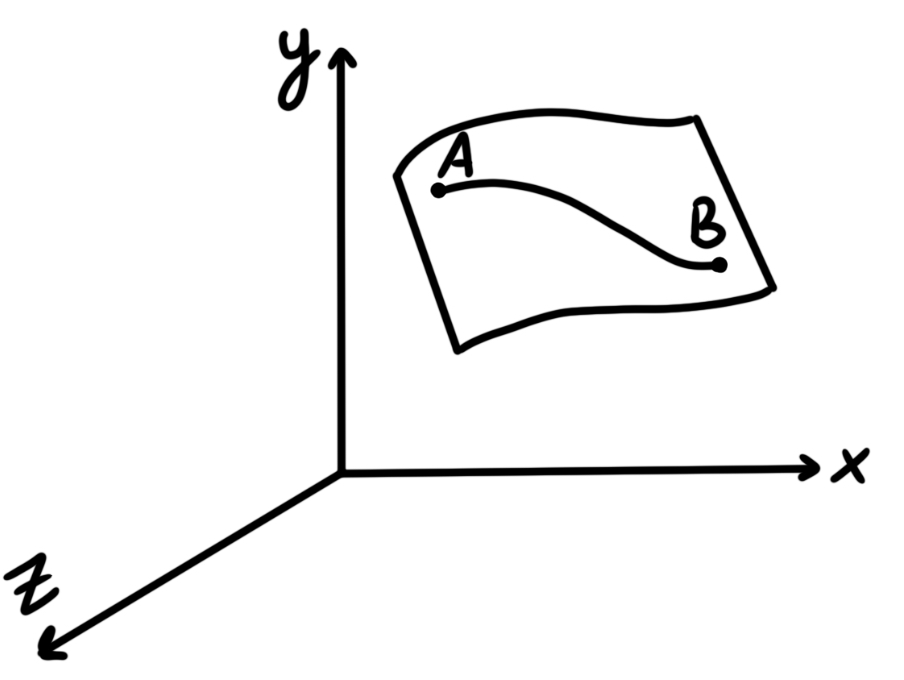
\includegraphics[width=0.4\textwidth]{/Users/vladbelousov/Desktop/Semestr_4-FP-NSU/ДфУ/Лекции_по_дням/image/4.png}
\end{center}
\begin{gather*}
    G(x,y,z)=0 - \text{уравнение поверхности} \\ 
    \text{Пусть уравнение кривой }:
    \begin{cases}
        x=x(t) \\
        y=y(t) \quad \quad t \in  [t_0,t_1] - \text{параметр} \\
        z= z(t)
    \end{cases}\\
    G(x(t),y(t),z(t)) = 0 \leftarrow \text{кривая лежит на поверхности}  \\
    l= \sum  \Delta l = \sum \sqrt{(\Delta x) ^2 + ( \Delta y ) ^2 + ( \Delta z ) ^2}=\sum  \sqrt{\left( \frac{\Delta x}{\Delta t} \right) ^2 + \left( \frac{\Delta y}{\Delta t} \right) ^2 + \left( \frac{\Delta z}{\Delta t} \right) ^2} \Delta t \\
    l \xrightarrow{\Delta t \to  0}    \int_{t_0}^{t_1} \sqrt{(x'(t)) ^2 + ( y'(t)) ^2 + ( z' ( t)) ^2 }dt  
\end{gather*}

\section{Простейшая задача вариационного исчисления}

\[ I[y]= \int_{x_0}^{x_1} F ( x, y(x),y'(x))dx \quad \quad \quad \quad (1)  \] 

\( F : \mathbb{D} \to \mathbb{R}, \mathbb{D} \subset \mathbb{R} ^3   \) непустое открытое множество, \( F \in  C ^2 (\mathbb{D}) \) 

\begin{definition}[допустимая функция]   
    Функция \( y : [x_0,x_1]\to \mathbb{R}  \) называется допустимой, если: 
    
    1) \(\displaystyle  y(x)\in  C([x_0,x_1]) \)
    
    2) \(\displaystyle  y(x) \in  C ^2 ((x_0,x_1)) \)
    
    3) \( \displaystyle \forall x \in  [x_0,x_1 ] , ( x, y(x), y ' (x)) \in  \mathbb{D}  \)
    
    4) \( \displaystyle \int_{x_0 }^{x_1} F(x,y(x),y' (x))dx \)  сходится

\end{definition}



\[ \text{Краевые условия: } y(x_0)=y_0,\text{ }  y(x_1)=y_1 \quad \quad \quad \quad (2) \] 

\begin{definition}
    Допустимая \( \tilde{y}:[x_0,x_1] \to  \mathbb{R}  \) доставляет локальный минимум функционалу (1) при краевых условиях (2),если: 

    1) \( \tilde{y}(x_0)=y_0, \tilde{y}(x_1)= y_1   \) 

    2) \( \exists \varepsilon_0 >0 \text{ }  \forall   \) допустимой функции \( y(x) \), удовлетворяющей (2): \( \sup _{x \in  [x_0,x_1]}|y(x)-\tilde{y}(x) |< \varepsilon_0  \) выполняется: \( I[\tilde{y}] \le I[y] \) 
\end{definition}

\begin{definition}
    Допустимая функция \( \tilde{y} : [x_0,x_1] \to  \mathbb{R} \)  доставляет глобальный минимум функционалу I[y] при краевых условиях (2), если: 

    1) \( \tilde{y} (x_0)=y_0, \text{ } \tilde{y} (x_1) =y_1 \)
    
    2) \( \forall \) допустимой функции \( y(x) \), удовлетворяющей (2), выполняется \( I[\tilde{y} ] \le I [y] \) 
\end{definition}

\section{Необходимые условия локального экстремума}

Аналог \( f'(x) = 0  \) 

Пусть функция \(\tilde{y}   \) доставляет функционалу \( I[y] \) при краевых условиях (2) локальный минимум \( \Rightarrow I[\tilde{y} ] \le I[y]  \), где \( y(x) \) из определенного локального минимума.

Возьмем \( \displaystyle y(x)=\tilde{y} + \varepsilon \eta(x) , \quad \varepsilon \in \left( -\frac{\varepsilon_0}{M}, \frac{\varepsilon_0}{M}   \right), \quad  M= \max _{x \in  [x_0,x_1]} |\eta (x) |  \)

\( \eta (x) \in  C ^2 ([x_0,x_1])  \) - финитная функция. 

\begin{minipage}{0.4\textwidth}
    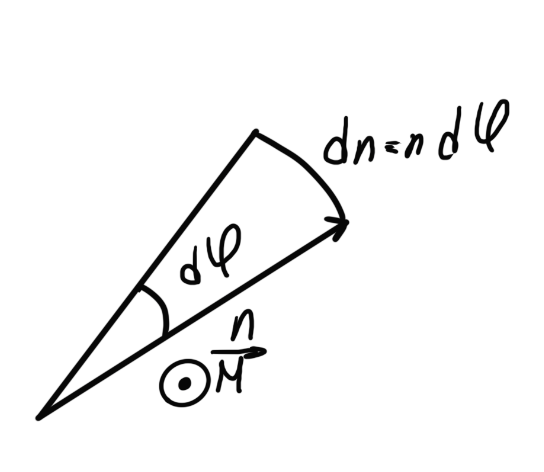
\includegraphics[width=\textwidth]{/Users/vladbelousov/Desktop/Semestr_4-FP-NSU/ДфУ/Лекции_по_дням/image/5.png}
\end{minipage}
\begin{minipage}{1\textwidth}
    \( \quad \quad \quad  \Rightarrow I[\tilde{y} ] \le I[\tilde{y} + \varepsilon \eta ]  \) 
\end{minipage}

Рассмотрим функцию \( g(\varepsilon)= I[\tilde{y}+ \varepsilon \eta  ] \Rightarrow g(0) \le g(\varepsilon) \) 

\begin{minipage}{0.25\textwidth}
    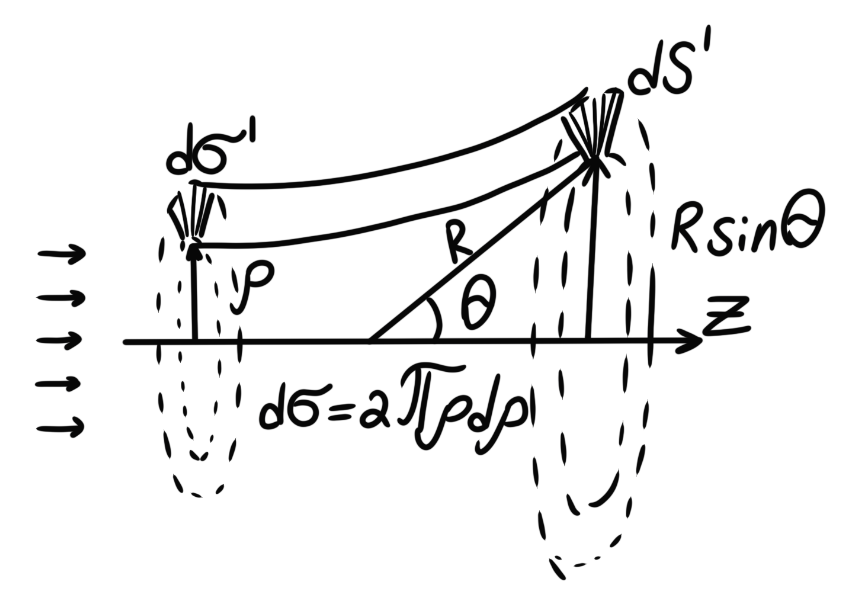
\includegraphics[width=\textwidth]{/Users/vladbelousov/Desktop/Semestr_4-FP-NSU/ДфУ/Лекции_по_дням/image/6.png}
\end{minipage}
\begin{minipage}{1\textwidth}
    \( \quad \varepsilon= 0 - \text{ точка локального минимума для функции } g(\varepsilon) \Rightarrow g'_{\varepsilon}(0)=0     \) 
\end{minipage}

\begin{gather*}
    0 = \frac{d}{d \varepsilon}g (\varepsilon) |_{\varepsilon=0}= \frac{d}{d \varepsilon} \left[ \int_{x_0}^{x_1} F(x,\tilde{y}+ \varepsilon\eta  (x) , \tilde{y}'+\varepsilon\eta ' (x) ) dx \right] \bigg |_{\varepsilon=0} \boxed{=}   \\
    \int_{x_0}^{x_1}= \underbrace{\int_{x_0}^{x_0+\delta} }_{(1)} +   \underbrace{\int_{x_0 +\delta}^{x_1-\delta} }_{(2)}  +\underbrace{\int_{x_1 -\delta}^{x_1} }_{(3)} \quad ; \quad \frac{d}{d \varepsilon} I_1= \frac{d}{d \varepsilon} I_2=0 \\   
\end{gather*}
\begin{theorem}[из математического анализа]
    \( f(x, \varepsilon): [a,b] \times [c,d] \to \mathbb{R}  \) - непрерывна, \( \displaystyle \exists  \frac{df}{d \varepsilon} (x, \varepsilon)   \)  - непрерывна
    \[ \Rightarrow \frac{d}{d \varepsilon} \int_{a}^{b} f(x, \varepsilon)dx= \int_{a }^{b } \frac{d}{d \varepsilon } f(x, \varepsilon)dx     \]  
\end{theorem}  

Вносим производную под знак интеграла: 

\begin{gather*}
    \boxed{=} \int_{x_0 + \delta}^{x_1- \delta}\left[ \frac{\partial F}{\partial y }(\dots) \eta (x )+ \frac{\partial F}{\partial y'} \eta '(x)   \right] dx \bigg |_{\varepsilon=0}=   \int_{x_0 + \delta}^{x_1- \delta}\frac{\partial F}{\partial y }(\dots) \eta (x )dx+ \underbrace{\frac{\partial F}{\partial y'}(x) \eta (x) \bigg |^{x_1- \delta}_{x_0+\delta}    }_{=0}- \\
    -\int_{x_0 + \delta}^{x_1- \delta} \eta (x )\frac{d}{dx } \left[ \frac{\partial F}{\partial y' }(\dots) \right] dx \bigg | _{\varepsilon=0} =\int_{x_0 + \delta}^{x_1- \delta} \left[ \frac{\partial F}{\partial y}(\dots)- \frac{\partial}{\partial x} \frac{\partial F}{\partial y'}(\dots)    \right]\eta(x) dx \bigg |_{\varepsilon=0}  \boxed{=}  \\
    \boxed{=} \int_{x_0 }^{x_1} \eta(x) \left[ \frac{\partial F}{\partial y}(x,y(x),y'(x)) -  \dots \right] dx =0
\end{gather*}

\( \forall   \) финитной функции \( \eta (x)  \)

\begin{lemma}[основаная леммая вариационного исчисления]
    \( f(x) : [x_0,x_1] \to  \mathbb{R} -\) непрерывна и  \( \displaystyle \int_{x_0}^{x_1} f(x)\eta (x)dx=0, \forall   \) финитной \( \eta (x) \). Тогда \( f(x) \equiv 0 \text{ } \forall x \in  [x_0,x_1]   \) 
\end{lemma}

По лемме: \( \displaystyle \frac{\partial F}{\partial y}- \frac{d}{dx} \frac{\partial F}{\partial y '} =0     \) - необходимое условие локального экстремума( \textbf{уравнение Эйлера} )

\begin{definition}[экстремаль]
    Допустимая функция \( y(x) \) называется экстремалью функционала \( I[y] \)  при краевых условиях (2), если: 

    1) \( y(x_0)=y_0, \text{ } y(x_1)=y_1  \) 

    2) \( y(x) \) удовлетворяет условию Эйлера
\end{definition}


%%-------------------------------%%

% Закрытие документа, если файл компилируется отдельно
\ifdefined\mainfile
    % Если это основной файл, не нужно заканчивать документ
\else
    \end{document}
\fi
% Условная компиляция для самостоятельной работы
\ifdefined\mainfile
    % Если это часть основного файла, не добавляем начало и конец документа
\else
    \documentclass[12pt, a4paper]{report}
    \usepackage{/Users/vladbelousov/Desktop/Semestr_4-FP-NSU/Настройка/library}
    \usepackage[utf8]{inputenc} % Подключение поддержки UTF-8
    \begin{document}
\fi

%%-------------------------------%%

\[ \begin{aligned}
\begin{cases}
    \displaystyle I[y] = \int_{x_0}^{x_1} F(x,y(x),y'(x))dx \\
    y(x_0)=y_0, \text{ } y(x_1)=y_1
\end{cases}
\quad (1)
\end{aligned} \] 

Найти функцию \( y(x) \)   такую, чтобы функционал \( I[y] \) принимал наибольшее или наименьшее значение. 

Необходимо найти условие локального экстремума: 

Если \( \tilde{y }       \)  экстремум \( \Rightarrow \tilde{y }  \frac{\partial F }{\partial y} - \frac{d}{dx }  \frac{\partial F}{\partial y '} = 0 \quad (2)   \)

\begin{proof}[Докозательство формулы (2)]
    \[ I[\tilde{y}] \le I[y] , y = \tilde{y} + \varepsilon \eta , \varepsilon \in  (- \varepsilon_1, \varepsilon_1), \eta(x) \in C^2([x_0,x_1])  - \text{финитная }    \] 
    
    \begin{center}
        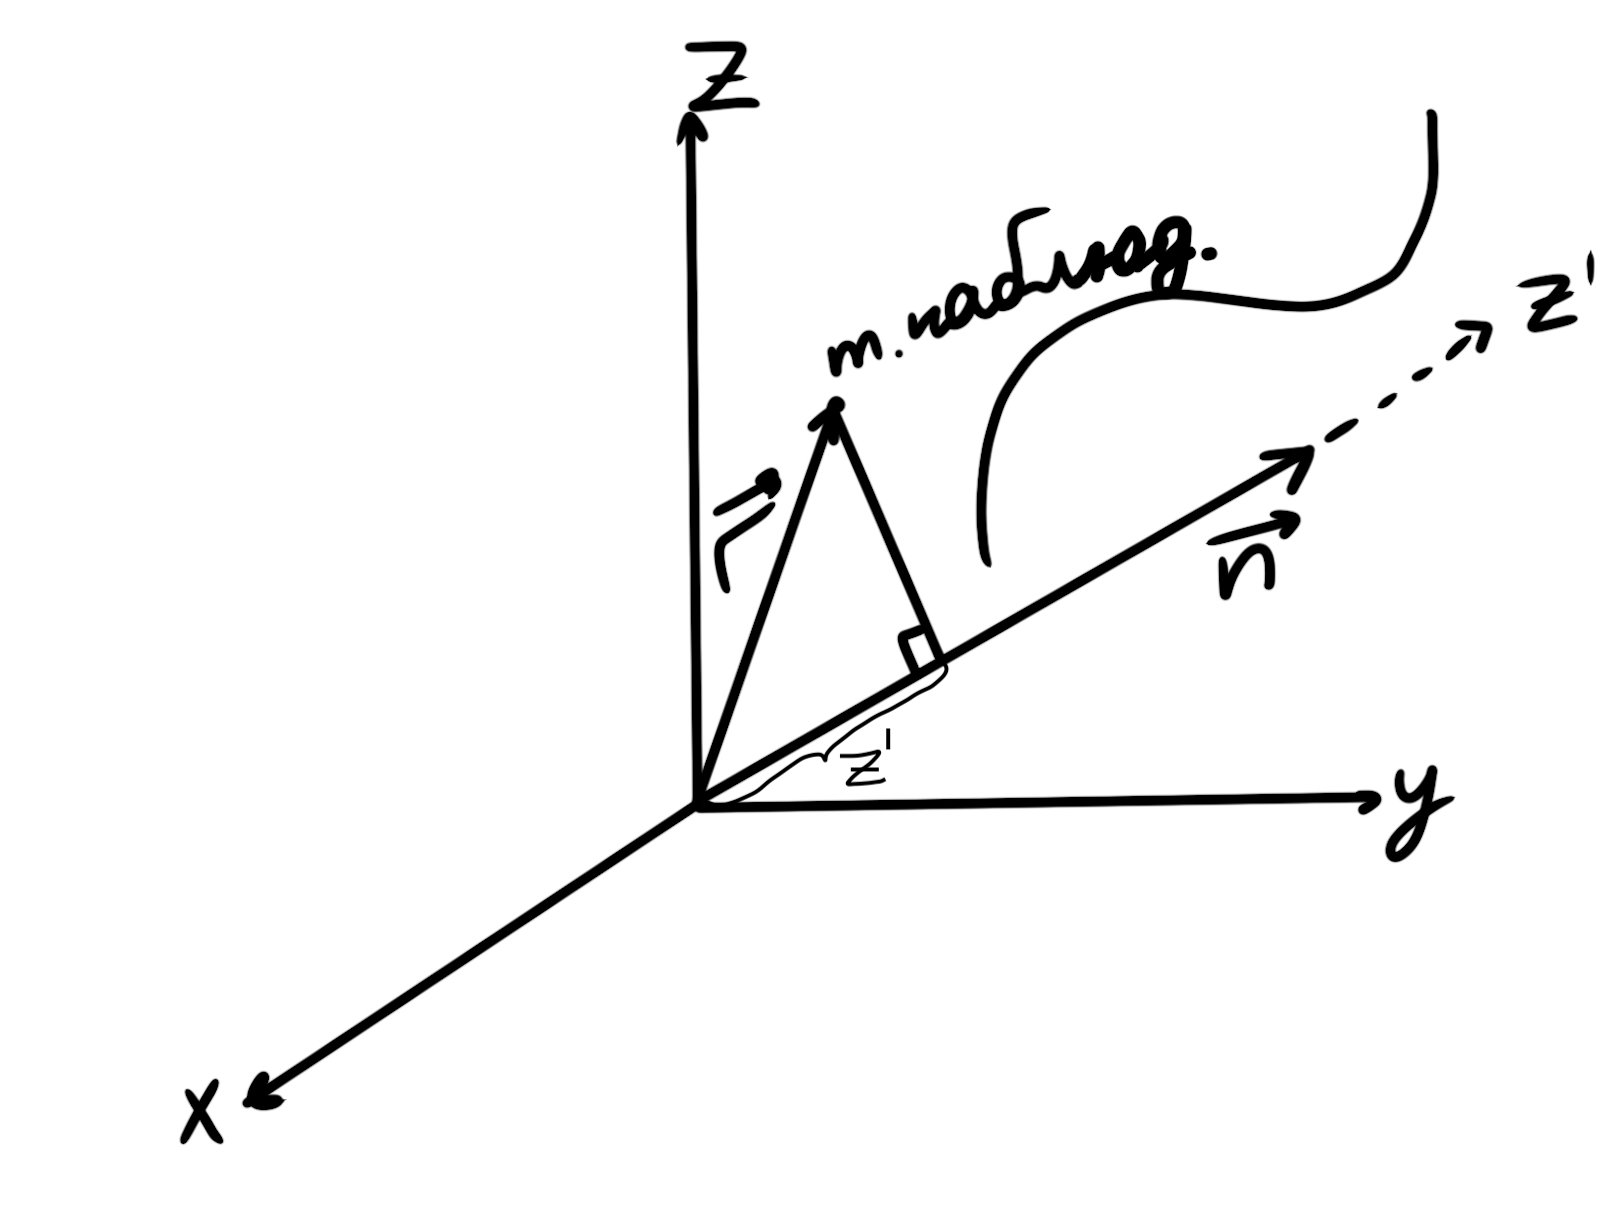
\includegraphics[width=0.3\textwidth]{/Users/vladbelousov/Desktop/Semestr_4-FP-NSU/ДфУ/Лекции_по_дням/image/7.png}
    \end{center}

    \[ \underbrace{I[y]}_{= g(0)} \le \underbrace{I[\tilde{y}+ \varepsilon \eta ]}_{=g(\varepsilon)} \Rightarrow g(0) \le g(\varepsilon) \Rightarrow g'( 0) = 0\] 

    \[ 0= \frac{d}{d \varepsilon} g(\varepsilon) |_{\varepsilon= 0 }= \int_{x_0}^{x_1} \left( \frac{\partial F }{\partial y } ( x , \tilde{y}(x) , \tilde{y }' (x) ) - \frac{d}{dx }  \frac{\partial F }{\partial y' } ( x , \tilde{y}(x) , \tilde{y }' (x) )  \right) \eta (x) dx , \forall \eta (x)  - \text{финитная}    \] 

    \begin{lemma}[Лагранжа]     
        Пусть \( f(x) \) - непрерывна и \( \displaystyle \int_{x_0}^{x_1} f(x) \eta (x) dx =0. \forall \eta (x) \) - финитная на \( [x_0,x_1] \). Тогда \( f(x) = 0 , \forall x \in  [x_0,x_1] \) 
    \end{lemma}

    \begin{proof}
        От противного:
        \begin{center}
            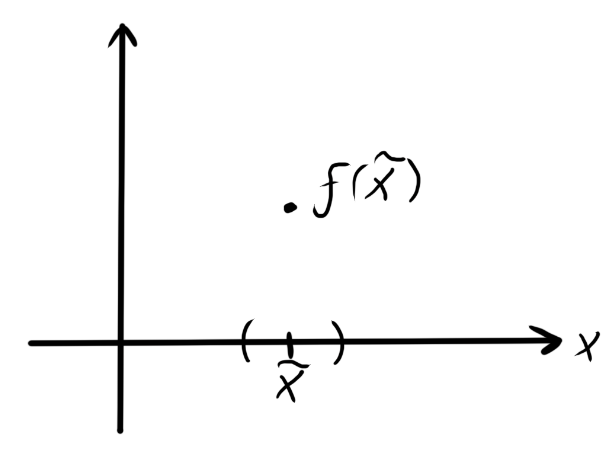
\includegraphics[width=0.3\textwidth]{/Users/vladbelousov/Desktop/Semestr_4-FP-NSU/ДфУ/Лекции_по_дням/image/8.png}
        \end{center}
        Пусть для определенности \( f(\tilde{x } )> 0        \) . Тогда так как \( f(\tilde{x}) \) - непрерывна, то \( f(x)>0    \) при \( x \in (\tilde{x}- \delta_0, \tilde{x}+\delta_0) \) 

        Возьмем функцию \( \eta(x) = \begin{aligned}
            \begin{cases}
                (\delta_0 ^2 - (x- \tilde{x})) ^ 4 , |x- \tilde{x}|< \delta   \\
                0 , |x- \tilde{ x } | > \delta_0
                \end{cases}
                - \text{финитная функция} 
        \end{aligned}\)
        
        \begin{center}
            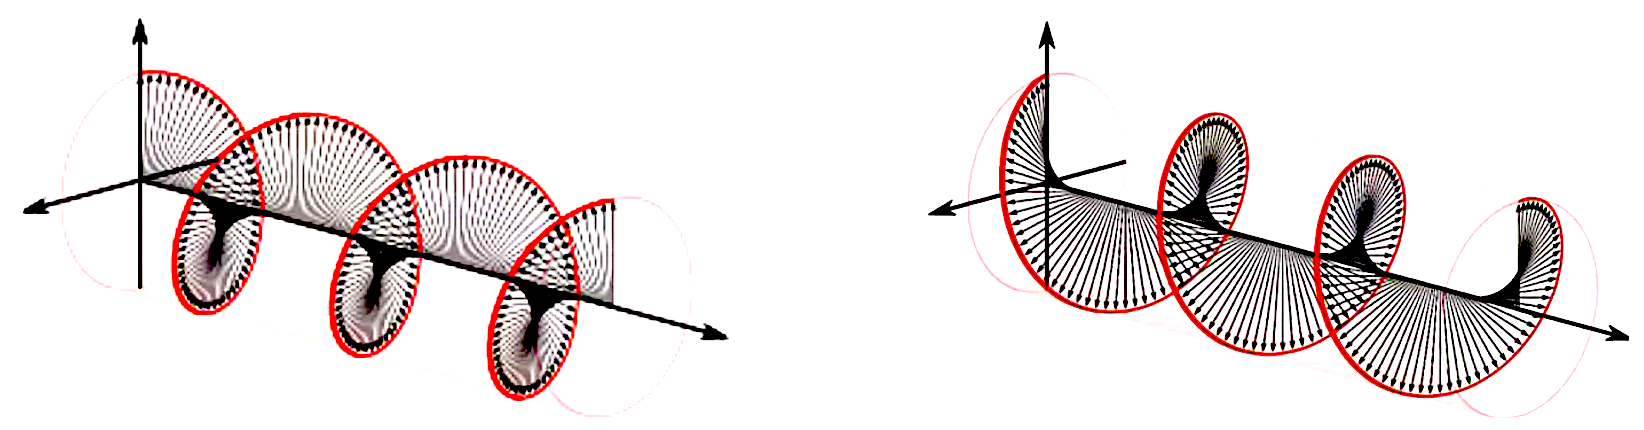
\includegraphics[width=0.3\textwidth]{/Users/vladbelousov/Desktop/Semestr_4-FP-NSU/ДфУ/Лекции_по_дням/image/9.png}
        \end{center}

        \[ \int_{ x_0 }^{x_1} f(x ) \eta(x ) dx = \int_{x_0 - \delta_0}^{x_1- \delta_0} \underbrace{f(x)}_{>0} \underbrace{\eta( x)}_{>0} dx >0 - \text{противоречие}    \] 

        \[ \Rightarrow \forall x \in  [x_0, x_1] : f(x) = 0  \] 
    \end{proof}

    Из доказательства леммы следует, что доказана формула (2)
\end{proof}

\section{Случай понижения порядка в уравнении Эйлера}   

\[ \frac{\partial F}{\partial y} - \frac{d}{d x }  \frac{\partial F}{\partial y'} = 0 \quad  F=F(x,y(x),y'(x))  \] 

1) \(\displaystyle  F= f(x,y) \Rightarrow \frac{\partial F }{\partial y} (x,y) =0 \Rightarrow y= y(x)    \) 

2) \( \displaystyle F= F (x, y ') \Rightarrow \frac{d}{dx }  \frac{\partial F }{\partial y'} (x,y') =0 \Rightarrow \frac{\partial F }{\partial y'} (x,y') = C    \) 


3) \( F= F( y , y ') \) :

\[ \frac{\partial F }{\partial y } - \frac{d}{dx }  \frac{\partial F }{\partial y '} = 0 | \cdot y '     \] 

\[ y' \frac{\partial F }{\partial y } - \underbrace{y ' \frac{ \partial F }{\partial y '}}_{= \frac{d}{dx } \left( y ' \frac{\partial F }{\partial y '} \right)- y'' \frac{\partial F }{\partial y '} }    = 0 \] 

\[ y' \frac{\partial F }{\partial y } - \frac{d}{dx } \left( y ' \frac{\partial F }{\partial y '}  \right)+ y'' \frac{\partial F }{\partial y '}  = 0 \] 

Заметим, что: \( \displaystyle \frac{d}{dx }F(y,y')  = y' \frac{\partial F }{\partial y } + y '' \frac{\partial F }{\partial y '}   \) 

\[ \frac{d}{dx }  F - \frac{d}{dx } \left( y ' \frac{\partial F }{\partial y '}           \right) = 0 \Rightarrow \boxed{F- y ' \frac{\partial F }{\partial y '} = C}   \] 


\section{Решение задачи о брахистохроне}

\begin{center}
    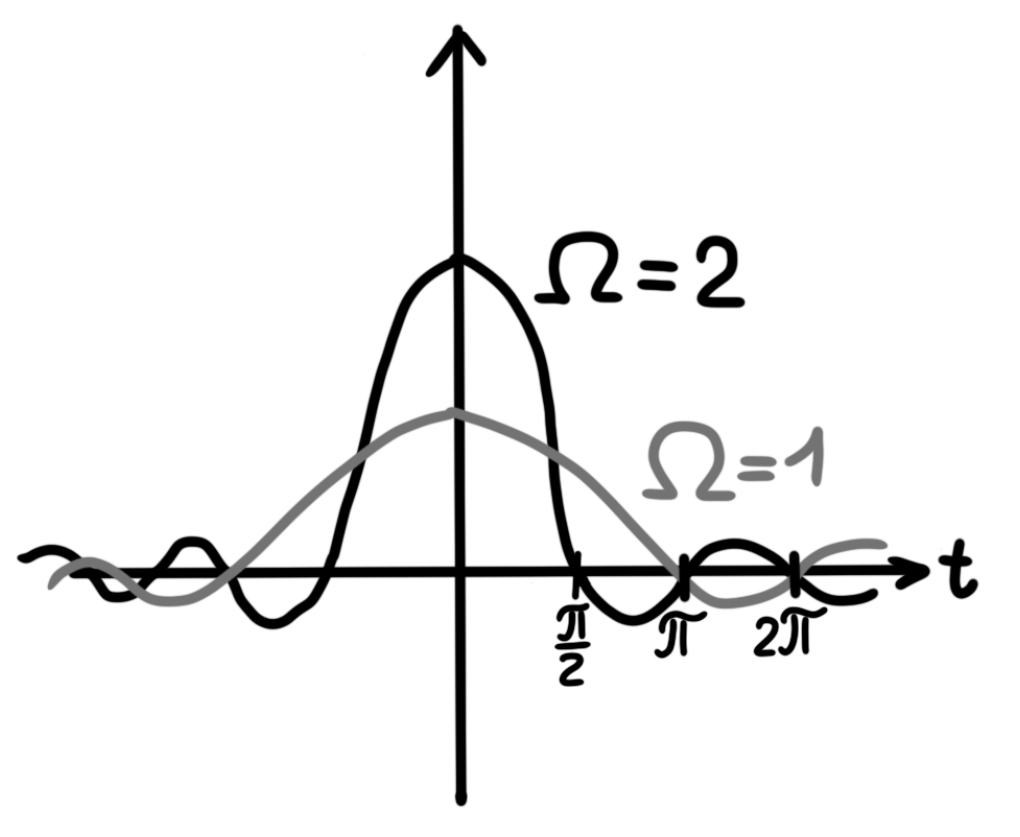
\includegraphics[width=0.3\textwidth]{/Users/vladbelousov/Desktop/Semestr_4-FP-NSU/ДфУ/Лекции_по_дням/image/10.png}
\end{center}

\[ \begin{cases}
\displaystyle I[y] = \int_{x_0}^{x_1} \frac{\sqrt{ 1+ (y ' (x)) ^2 )}}{\sqrt{2 g (y_0 - y (x))}} dx \\
y(x_0) = y_0, \text{ } y(x_1) = y_1
\end{cases} \] 

\[ \frac{\sqrt{1+ ( y ' ) ^2 } }{ \sqrt{2 g ( y_0 - y )} } - y ' \frac{1}{\sqrt{1+ ( y ' ) ^2 }} \frac{2 y '}{2 \sqrt{1 +( y ') ^2 } } = C    \] 

\[ \underbrace{\sqrt{1+ ( y ' ) ^2 } - (y ') ^2 \frac{1}{ \sqrt{1 + (y') ^2}}}_{\displaystyle \frac{1}{\sqrt{1+ (y ') ^2 }} } = C \sqrt{2g (y_0 - y )}  \] 

\[ 1= \underbrace{c ^2 2g}_{= \frac{1}{c_1}>0 } ( y_0 - y)( 1+ (y ') ^2) \] 

\[ c_1= (y_0 - y )(1 + ( y ' ) ^2 ) \Rightarrow \pm \sqrt{\frac{c_1}{y_0 - y }-1} = y ' \quad (3 )  \] 

\begin{center}
    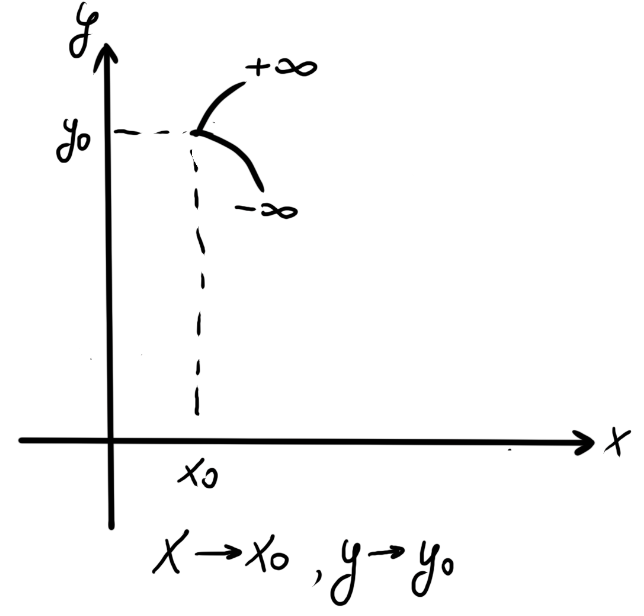
\includegraphics[width=0.3\textwidth]{/Users/vladbelousov/Desktop/Semestr_4-FP-NSU/ДфУ/Лекции_по_дням/image/11.png}
\end{center}

\[ 1+(y'(x)) ^2 = \frac{c_1}{y_0 - y(x)} \xrightarrow{x \to x_1} + \infty     \] 

\[ y ' ( x ) \xrightarrow{x \to  x_0} \underset{{\small \text{выбор}} : - }{\pm \infty}  \Rightarrow y ' (x )  \xrightarrow{x \to  x_0} - \infty      \] 

\[ y ' = - \sqrt{\frac{c_1- y_0 + y }{y_0 - y } } \] 

Замена: \( \tilde{y }= y_0 - y (x) \):

\[ \tilde{y} '(x) = + \sqrt{\frac{c_1 - \tilde{y }}{\tilde{y }} }  \] 

Замена: \( \tilde{y } = c_1 z \): 

\[ c_1 z ' = \sqrt{\frac{c_1 - c_1 z }{c_1 z } }= \sqrt{\frac{1-z}{z } } \] 

Замена: \( z= \sin ^2 s, s \in  \left[ 0 , \frac{\pi}{2}  \right] \) 

\[ c_1 2 \sin s \cos s \cdot s' = \sqrt{ \frac{1- \sin ^2 s }{\sin ^2 s } }= \frac{\cos s }{\sin s } \text{ } (\text{знак определили из интервала s} )   \] 

\[ 2 c_1 \sin ^2 s \frac{ds}{dt } =1     \] 

\[ \frac{dx }{ds }  = c_1 ( 1 - \cos (2s) ) \Rightarrow \boxed{x(s) = c_1 \left( s - \frac{1}{2 }  \sin 2s  \right)- c_2} -   \] 

\[ y(x )= y_0 - \tilde{y } (x ) = y_0 - c_1z= y_0 - c_1 \sin ^2 s = y_0 - \frac{c_1}{2} ( 1 - \cos  2s) \]  

\[ \boxed{y(s )= y_0 - \frac{c_1}{2 }  ( 1 - \cos (2s))}   \] 

Замена: \( t = 2s , \text{}  t \in  ( 0 , \pi) \) 

\[ \begin{aligned}
    \begin{cases}
        \displaystyle x(t) = \frac{c_1}{ 2 }  ( t - \sin t ) + c_2  \\ 
        \displaystyle y(t)= y_0 - \frac{c_1}{2 }  ( 1 - \cos t)
    \end{cases}
    \quad , \quad t \in ( 0 , \pi)
\end{aligned} \]

\[ \begin{pmatrix}
x(t )\\
y (t)
\end{pmatrix} = \begin{pmatrix}
\frac{c_1}{2 }  + c_2 \\
y - \frac{c_1}{2} 
\end{pmatrix}= \begin{pmatrix}
-\frac{c_1}{2 } \sin t\\
\frac{c_1}{2}  \cos t 
\end{pmatrix} \quad t \in  (0 , \pi)\] 

\begin{center}
    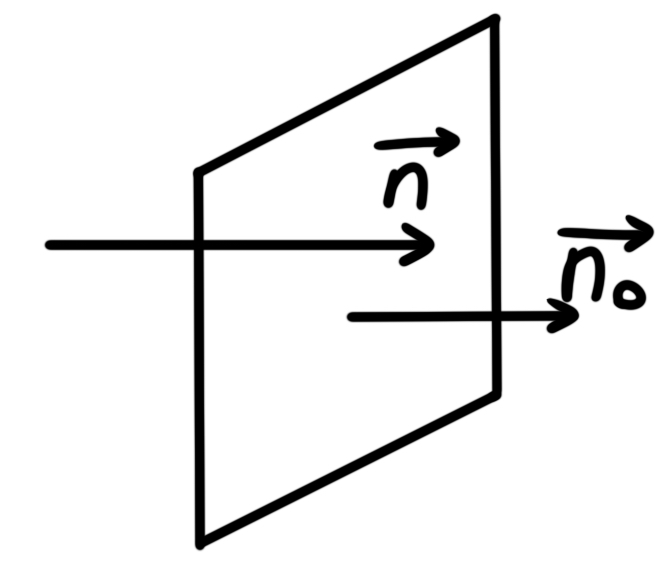
\includegraphics[width=0.5\textwidth]{/Users/vladbelousov/Desktop/Semestr_4-FP-NSU/ДфУ/Лекции_по_дням/image/12.png}
\end{center}

\[ \begin{aligned}
    t= 0 : 
    \begin{cases}
        x(0 ) = c_2 = x_0 \\
        y(0 ) = y_0
    \end{cases}
\end{aligned} \] 

\[ \begin{aligned}
    t= \pi: 
    \begin{cases}
        x(\pi ) = \frac{c_1}{2 }  \pi + c_2= \frac{c_1}{2 } \pi + x_0  \\
        y(\pi) = y_0 - c_1
    \end{cases}
\end{aligned} \] 

\begin{center}
    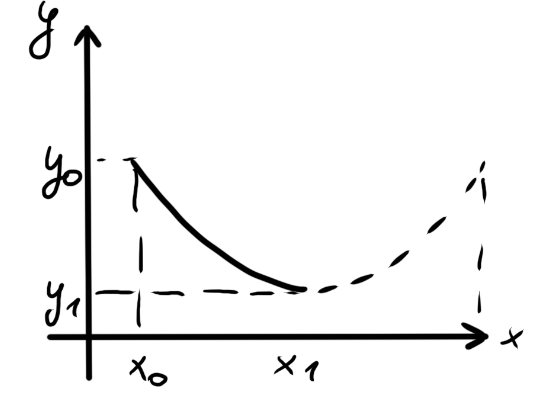
\includegraphics[width=0.3\textwidth]{/Users/vladbelousov/Desktop/Semestr_4-FP-NSU/ДфУ/Лекции_по_дням/image/13.png}
\end{center}

Теперь возьмем "+" ( формула (3)): 

\[ y ' = \sqrt{\frac{ c_1 - y_0 + y }{y_0 - y } }\quad (5 ) \] 

\[ \tilde{y } (x ) = y_0 - y (x ) \Rightarrow \tilde{y } ' = - \sqrt{\frac{ c- \tilde{ y } }{\tilde{y }}}   \]  

Делаем те же действия (замены) и получаем такие же \( x(s), y ( s ) \) с различием только в интервале для t: 

\[ \begin{aligned}
    \begin{cases}
        x(T)  = \frac{C_1}{ 2 }  ( t- \sin t ) + x_0 \\
        y(t ) = y_0 - \frac{c_1}{2 }  ( 1- \cos  t )            
    \end{cases}
    \quad ,\quad t \in ( 0 , 2 \pi ) \Rightarrow \text{ циклоида полная }  
\end{aligned} \]  

\begin{center}
    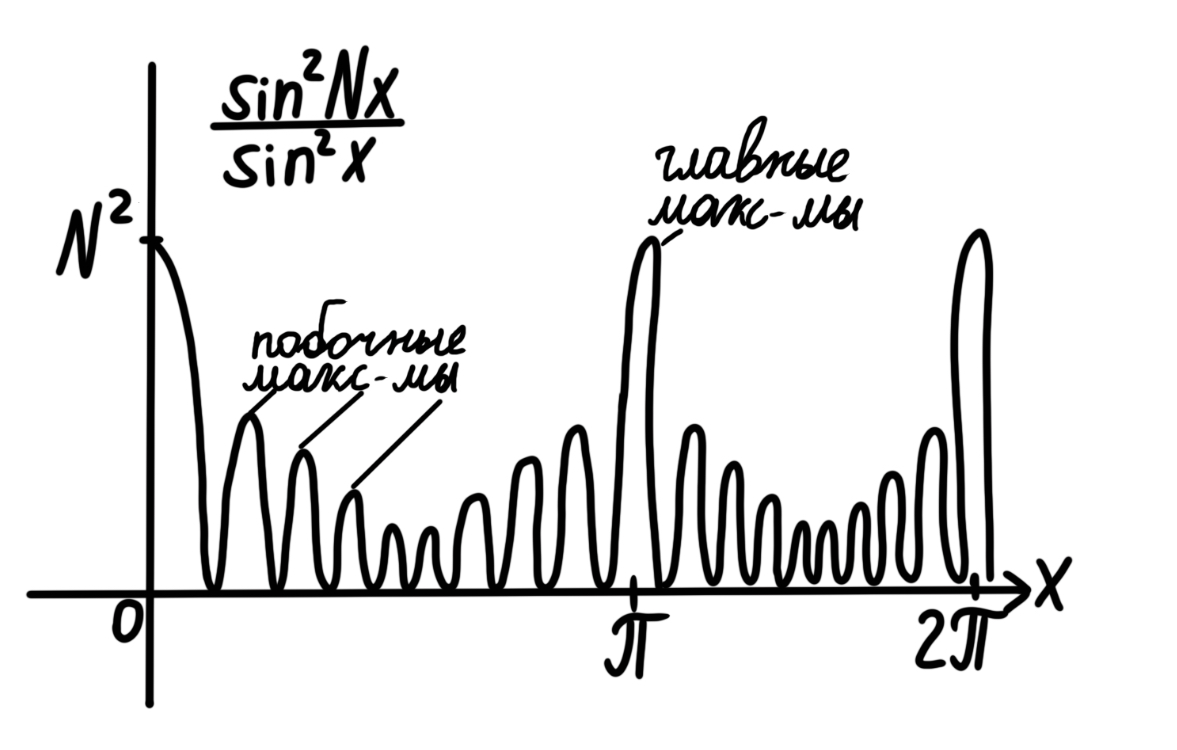
\includegraphics[width=0.5\textwidth]{/Users/vladbelousov/Desktop/Semestr_4-FP-NSU/ДфУ/Лекции_по_дням/image/14.png}
\end{center}

\newpage

\section{ Решение задачи о поверхности вращения наименьшей площади}

\begin{center}
    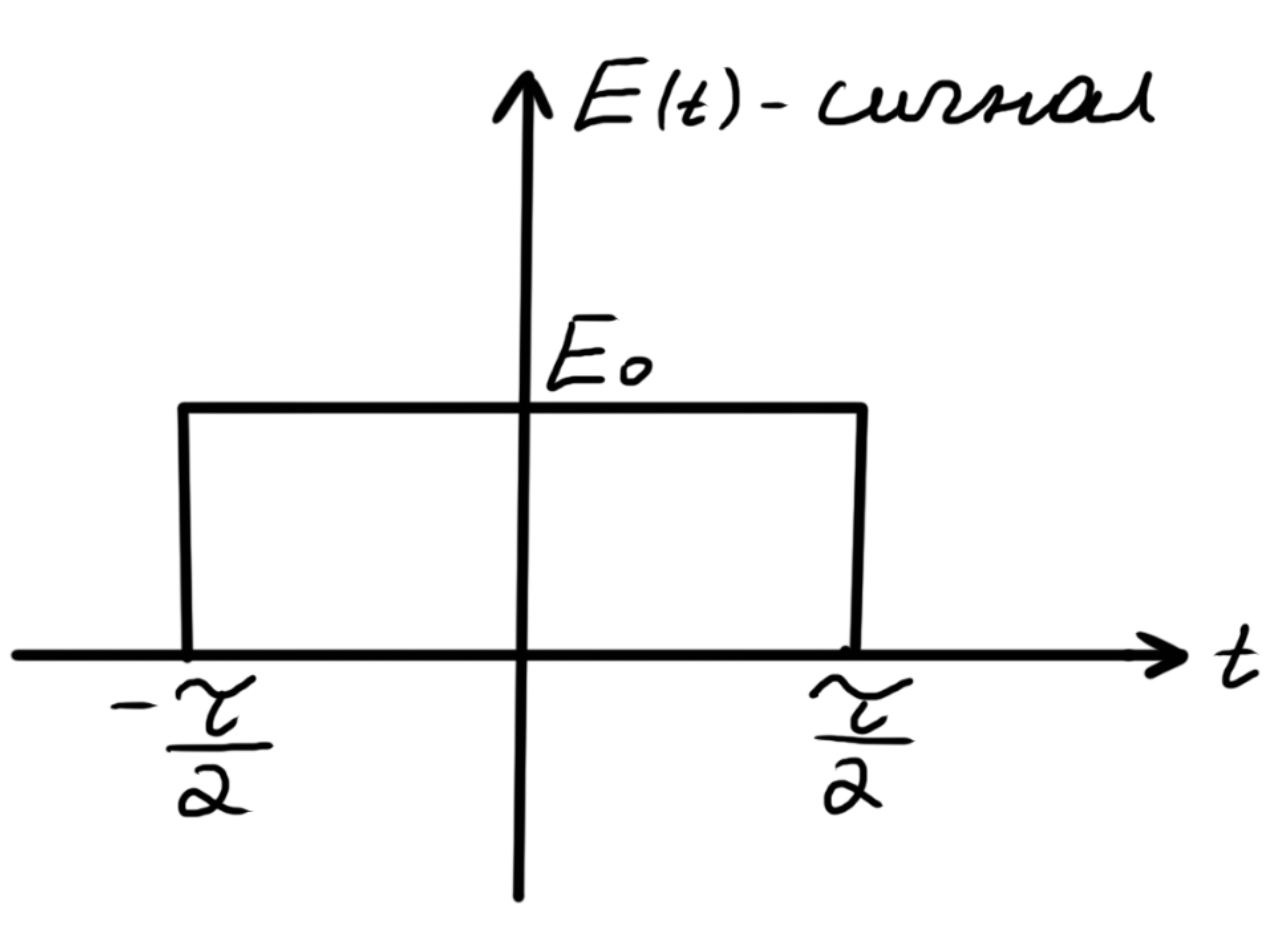
\includegraphics[width=0.3\textwidth]{/Users/vladbelousov/Desktop/Semestr_4-FP-NSU/ДфУ/Лекции_по_дням/image/15.png}
\end{center}

\[ \begin{cases}
I[ y ] = \int_{x_0}^{x_1} 2 \pi y(x )  \sqrt{1 + (y '(x ) ^2 )} \\ 
y( x_0 ) = y_0 , \text{ }  y ( x_1 ) = y_1 
\end{cases} \] 

\[ F- y; \frac{\partial  F }{\partial   y' } = C   \] 

\[ 2 \pi y \sqrt{ 1 + (y' ) ^2 } - y ' 2 \pi y \frac{2 y '}{ 2 \sqrt{1 + ( y ') ^2 }} = C  \] 

\[ 2 \pi y \underbrace{\left( \sqrt{1 + (  y') ^2 } - \frac{ (y ' ) ^2 }{\sqrt{1 + ( y ' ) ^2 }}  \right)}_{= \frac{1}{\sqrt{ 1 + ( y ' ) ^2 }} } = C \] 

\[ ( 2 \pi y  ) ^2 = c ^2 ( 1 + ( y '   ) ^2 ) \] 

1) \( c= 0 \Rightarrow y(x )  =0  \) - решение, если \( y_0 = y_1 = 0 \) 

2) \( c \neq 0 \Rightarrow \left(  \frac{y}{c_1 }     \right) ^2 = 1 + ( y ' ) ^2 \Rightarrow y ' = \pm  \sqrt{\frac{ y ^2 }{c_1 ^2} - 1  }, \text{ }  c_1 = \frac{c}{2 \pi} > 0         \) 

\[ y( x ) = \mathrm{ch}  z(x  ) c_1 , \text{ }  z> 0 \]  

\[ c_1 \mathrm{sh } z \cdot z ' (x )   =\pm \underbrace{ \sqrt{\mathrm{ch} ^2 z - 1  }}_{= \mathrm{sh} z  }   \Rightarrow c_1 z = \pm 1   \] 

\[ z= \pm  \frac{ x- c_2 }{c_1} \Rightarrow y ( x )  = c_1 \mathrm{ch} \left( \frac{x+c_2 }{c_1}  \right)  - \text{цепная линия}  \] 

\begin{center}
    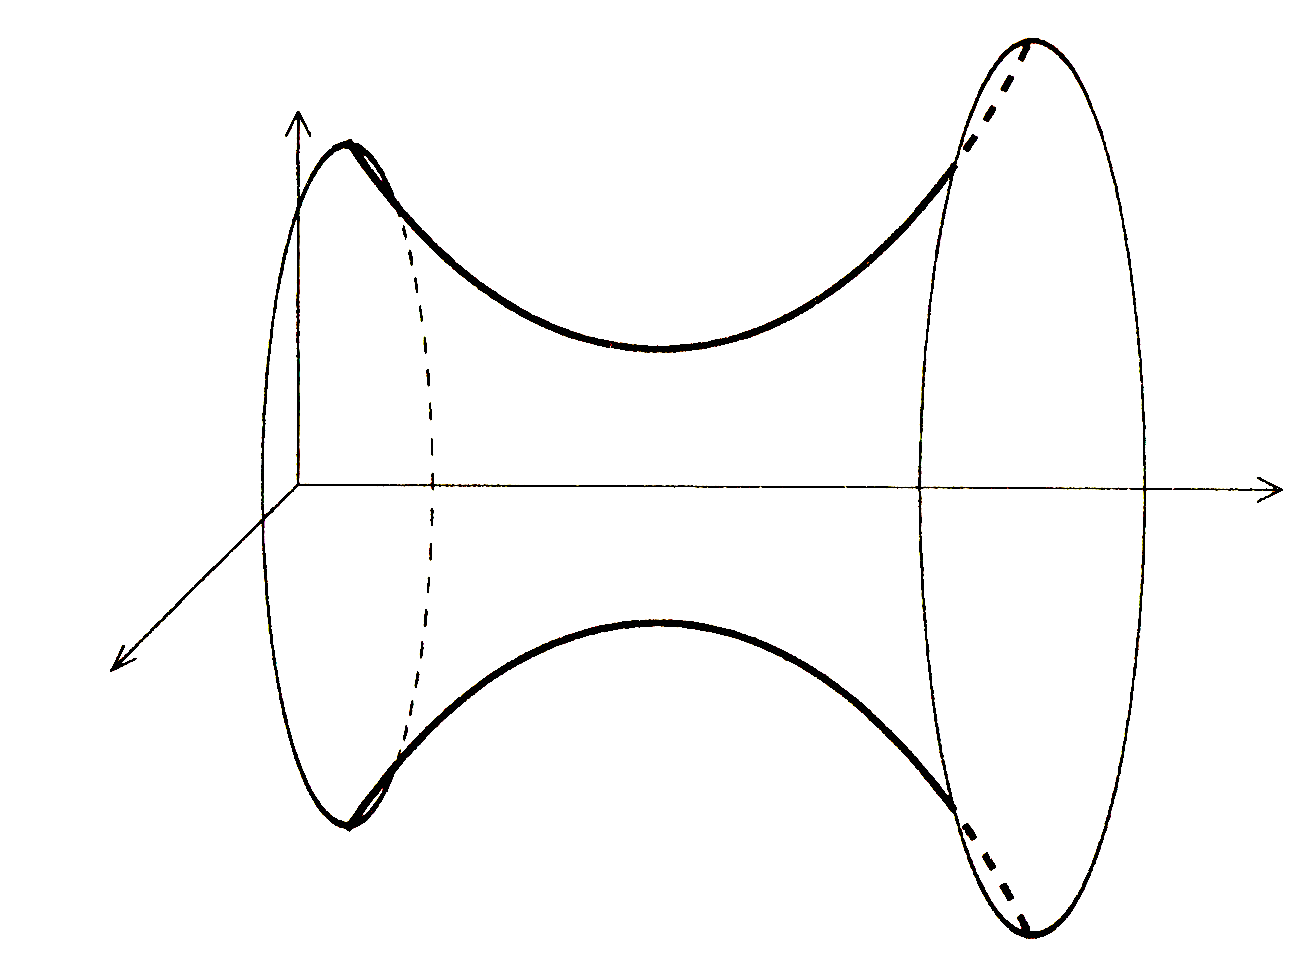
\includegraphics[width=0.4\textwidth]{/Users/vladbelousov/Desktop/Semestr_4-FP-NSU/ДфУ/Лекции_по_дням/image/16.png}
\end{center}



\section{Вариационная задача с несколькими функциями}

\[ I[y_1, \ldots, y_n ] = \int_{x_0 }^{x_1 } F(x,y_1(x),y_1 ' (x), \ldots , y_n ( x ) , y _n '( x))dx  \] 

\[ \begin{cases}
    y_1(x_0 ) = y_{01} , \ldots , y_n ( x_0 ) = y_{0n } \\
    y_1(x_1 ) = y_{11} , \ldots , y_n ( x_1) = y_{1n }
\end{cases} \] 

Необходимое условие локального экстремума: 

Пусть \( \tilde{y }_1 (x ) ,\ldots, \tilde{y }_n( x )  доставляет функционалу локальному экстремуму ему, то есть: \)

\[ I [\tilde{y }_1, \ldots , \tilde{y}_n  ] \le I[y_1, \ldots , y_n ] , \text{ }  \forall y_2, \ldots , y_n \] 

Можно взять \( y_1   \) - любое: \( y_2=\tilde{y}_2, \ldots ,   \) 

\[\Rightarrow \underbrace{ I[\tilde{y}_1, \ldots, \tilde{y   }_n ]}_{Y[\tilde{y } _1] } \le \underbrace{I[y_1, \ldots, \tilde{y  }_n ]}_{Y[y_1 ]} \Rightarrow \frac{\partial F }{\partial  y_1} - \frac{d}{dx }  \frac{\partial  F }{\partial  y_1 '}= 0     \]  

Аналогично: \( \frac{\partial F }{\partial  y_j }- \frac{d}{dx }  \frac{\partial F }{\partial  y ' _j} = 0   \) 


%%-------------------------------%%

% Закрытие документа, если файл компилируется отдельно
\ifdefined\mainfile
    % Если это основной файл, не нужно заканчивать документ
\else
    \end{document}
\fi
% Условная компиляция для самостоятельной работы
\ifdefined\mainfile
    % Если это часть основного файла, не добавляем начало и конец документа
\else
    \documentclass[12pt, a4paper]{report}
    \usepackage{/Users/vladbelousov/Desktop/Semestr_4-FP-NSU/Настройка/library}
    \usepackage[utf8]{inputenc} % Подключение поддержки UTF-8
    \begin{document}
\fi

%%-------------------------------%%

\section{ Вариационная задача с высшими производными }

\[ I[y ]= \int_{x_0 }^{x_1 } F( x, y (x), y' (x),..., y ^{(n )} (x))  dx\]  

\[ \begin{cases}
    y(x_0) = y_0 ,\quad  y (x_1) = y_1 \\
    y ' (x_0) = y ' _0 , \quad y ' (x_1) = y ' _1 \\
    \ldots 
    y^{(n )} = y^{(n )}_0, \quad y^{(n )} (x_1) = y^{(n )}_1
\end{cases} \]  

Необходимое условие локального экстремума: 

Если функция \( \tilde{y }(x ) \)  доставляет функционалу локальному экстремум, то \( \tilde{ y }(x) \)  - решение диффернциального уравнения

\[ \frac{\partial  F }{\partial  y } - \frac{d}{dx } \frac{ \partial  F }{\partial  y ' } + \frac{d ^2 }{dx ^2 } \frac{\partial  F }{\partial  y ''} + \ldots + \frac{d ^n }{dx ^n } \frac{\partial  F }{\partial  y ^{(n )}} = 0    \] 


\begin{proof}
     \[   \] 
    Пусть \( \tilde{y }( x) \)  доставляет функционалу локальный минимум \( \Rightarrow  \exists \varepsilon_0 >0 , \text{ }  \forall  y(x )\), удовлетворяет краевым условиям, \( \displaystyle \sup_{x \in [x_0 , x_1 ] } |y(x)-\tilde{y }(x) | < \varepsilon_0  \Rightarrow I[\tilde{y }] \le  I[y] \) 

    Возьмем \( y(x ) = \tilde{y }( x ) + \varepsilon \eta ( x ), \eta(x) \)  финитная функция.

    \[ \underbrace{I[\tilde{ y }]}_{g(0)} \le  \underbrace{I[\tilde{y }+ \varepsilon \eta ]}_{g(\varepsilon)} \Rightarrow g(0 ) \le  g(\varepsilon) \Rightarrow \varepsilon = 0  - \text{ точка локального минимума для функции } g(\varepsilon) \] 

    \[ g ' (0 ) = 0 \]  

    \[ 0 = \frac{d}{d \varepsilon } g(\varepsilon ) \bigg |_{\varepsilon = 0 }  = \frac{d}{d \varepsilon} \int_{x_0 }^{x_1} F ( x, \tilde{y }( x)  + \varepsilon \eta ( x ), \tilde{y }' ( x) + \varepsilon \eta' ( x ), ...) dx \bigg |_{\varepsilon = 0} \] 

    Если \( F \in C^{\infty  } (\mathbb{R} ^{n +2 } ), y(x ) \in C^{\infty  } ([x_0 , x_1 ])    \), то 

    \[ 0 = \int_{x_0 }^{x_1} \left[ \frac{\partial  F }{\partial  y } \eta( x) + \frac{\partial F }{\partial  y' }(... )\eta' ( x )+ \frac{\partial F }{\partial y ''} (...) \eta''(x) +\dots  \right]  dx \bigg | _{\varepsilon = 0 }  =    \] 

    \[ =\int_{x_0 }^{x_1}  \frac{\partial  F }{\partial  y } \eta ( x ) dx + \frac{\partial  F } {\partial  y ' } \eta  ( x ) \bigg |_{x_0 }^{x_1}   - \int_{x_0 }^{x_1} \eta( x ) \frac{d }{dx } \frac{\partial  F }{\partial  y ' } (... )dx + \frac{\partial  F }{ \partial  y ' } (... ) \eta ( x ) \bigg |_{x_0 }^{x_1} - \int_{x_0 }^{x_1}  \eta ' ( x ) \frac{d}{dx } \frac{\partial  F }{\partial  y ''} dx ... \text{ и тд}    \] 

    \[ = \int_{x_0 }^{x_1} \left(  \frac{\partial  F } {\partial  y } - \frac{d}{dx } \frac{\partial F }{\partial  y '}  \right) \eta(x )dx - \eta(x ) \frac{d}{dx } \frac{\partial F }{ \partial  y '}\bigg |_{x_0 }^{x_1 } \int _{x_0 }^{x_1} \eta  ( x ) \frac{d ^2 }{dx ^2 } \frac{\partial F }{\partial y ''} dx +... \text{ и тд }       =  \] 

    \[ =\int_{x_0 }^{x_1} \left(  \frac{\partial  F } {\partial  y } - \frac{d}{dx } \frac{\partial F }{\partial  y '} + \frac{d ^2 }{d x ^2 } \frac{\partial F }{\partial y ''}  \right) \eta(x )dx +...  = 0 \quad \forall \text{ финитной функции  } \eta( x) \] 

    Если n = 2 , то по лемме Лагранжа: \( \displaystyle  \frac{\partial  F } {\partial  y } - \frac{d}{dx }  \frac{\partial  F } { \partial y ' } + \frac{d ^2 }{dx ^2 }  \frac{\partial  F }{ \partial  y''}  =0   \) 

    При n > 2 аналогично.

\end{proof}


\section{Вариационная задача с несколькими независимыми переменными}

\[ \begin{cases}
    I [ z] = \iint_{D } F (x, y , z(x ), z_x ' ( x,y), z_y ' ( x,y )) dx dy \\
    z  | _{(x,y ) \in  \partial D } = \varphi ( x,y)
\end{cases} \] 

Необходимое условие локального экстремума: 

\[ \frac{\partial  F }{ \partial z } - \frac{\partial  }{\partial  x } \frac{\partial  F }{ \partial z_x ' } - \frac{\partial  }{\partial  y } \frac{\partial  F }{ \partial z_y ' } = 0    - \text{ уравнение Эйлера-Остроградского}   \] 

\textbf{Без доказательства} 

\section{Принцип Остроградского-Гамильтона (принцип наименьшего действия, признак стационарного действия, основной вариационный принцип механики)}

T - кинетическая энергия, U - потенциальная энергия: 

\[ L = T - U - \text{ Лагранжиан}  \] 

\[ S = \int_{t_0 }^{t_1} L dt - \text{функционал действия}  \] 

Движения в системе происходит  по экстремалям функционала действия. 

Пример: 

\begin{center}
    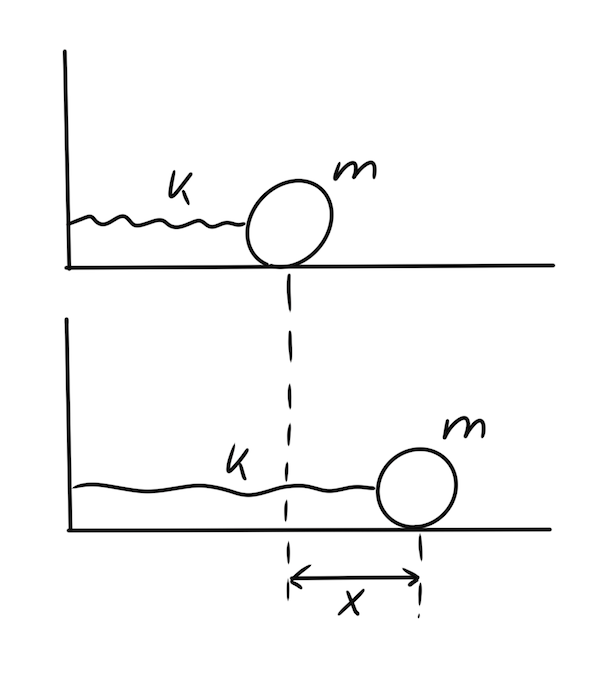
\includegraphics[width=0.3\textwidth]{/Users/vladbelousov/Desktop/Semestr_4-FP-NSU/ДфУ/Лекции_по_дням/image/17.png}
\end{center}

\[ T = \frac{m \dot{x } ^2 }{2} \quad  U = \frac{k x ^2 }{2}  \] 

\[ S = \int_{t_0 }^{t_1} \left( \frac{m \dot{x } ^2 }{2} -  \frac{k x ^2 }{2}\right)  dt \] 

Уравнение Эйлера (уравнение Лагранжа): \( \displaystyle  \frac{\partial L }{ \partial x  } - \frac{d}{dt} \frac{\partial L }{ \partial \dot{x}  } = 0  \) 

\[ - kx - \frac{d}{dt } ( m \dot{x } ) = 0  \Rightarrow m \ddot{x} + kx = 0  \] 

Понижение порядка: \( \displaystyle  L - \dot{x } \frac{\partial K }{\partial  \dot{x} } = C  \) 

\[ \frac{m \dot{x }  ^2 }{2 } - \frac{k x ^2 }{2 } - \dot{x } m \dot{x } = c \Rightarrow -\frac{m \dot{ x } ^2 }{2 } - \frac{k x ^2  }{2}  =c   \] 

\section{Изопериметрическая задача }

Найти кривую заданной длины, ограничивающую наибольшую площадь.

\[ \begin{aligned}
    S &\to  \max  \\ 
    l &= \mathrm{const}  
\end{aligned} \] 

\begin{center}
    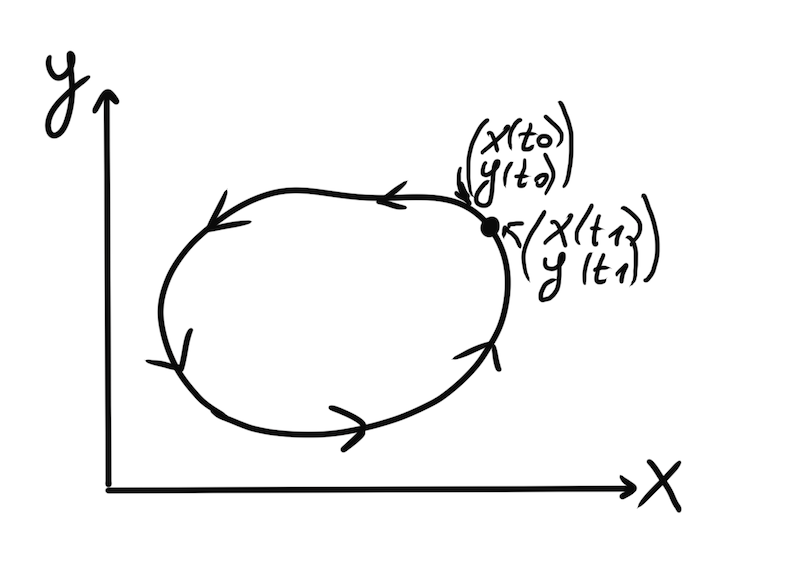
\includegraphics[width=0.5\textwidth]{/Users/vladbelousov/Desktop/Semestr_4-FP-NSU/ДфУ/Лекции_по_дням/image/18.png}
\end{center}

\[\begin{aligned}
    \begin{cases}
        x = x(t) \\ 
        y = y(t) \quad  t \in [ t_0 ,t_1]
        \end{cases}
    \begin{aligned}
        x(t_0 )=x(t_1) \\ 
        y(t_0 )=y(t_1) \\  
    \end{aligned}
\end{aligned} \]

\[ S = \iint_D dx dy   \] 

\[ \int_{ \partial D} \left( P(x,y )dx +Q(x,y )dy  \right) =\iint _D \left( - \frac{\partial P }{ \partial  y } (x,y ) + \frac{\partial Q}{\partial x }(x,y)   \right) dx dy\] 

\[ S = \iint_D dx dy = \iint_D \left(\underbrace{ \frac{1}{2 }}_{- \frac{\partial  P}{\partial y} } + \underbrace{ \frac{1}{2 }}_{ \frac{\partial  Q}{\partial x} }       \right)dx dy = \int_{ \partial  D } \left(  - \frac{y}{2 } dx + \frac{x}{2 } dy \right)  =\frac{1}{2 } \int_{t_0 }^{t_1} (x(t )y ' (t )- x' (t )y (t))dt  \] 

\[ \begin{cases}
\frac{\partial P } {\partial y } = -\frac{1}{2 }  \quad   \\
\frac{\partial Q }{\partial x } = \frac{1}{2 } \quad  Q = \frac{x}{2}   
\end{cases} \] 

\[ l = \int_{t_0 }^{t_1} \sqrt{(x' (t ) ^2 + (y '(t ) )^2 } dt = \mathrm{const}   \] 

Задача из математического анализа : 

\[ \begin{cases}
f(x_1, \ldots, x_n ) \to  \mathrm{extz}   \quad \quad  \tilde{f } =f + \lambda_1 g_1 + ... + \lambda_m g_m \to  \mathrm{extz}   \\
g_1 (x_1, \ldots, x_n ) = 0 \\
\vdots \\
g_m (x_1, \ldots, x_n ) = 0
\end{cases} \] 

Задача вариационного исчисления: 

\[ I[y_1, \ldots, yn] = \int_{x_0 }^{x_1 } F(x,y_1, \ldots, y_n,y_1',..., y_n') dx \to  \mathrm{extz}   \] 

\[ \begin{cases}
y_1(x_0 ) = y_0 ^1 \quad  y_n(x_0 ) = y_0 ^n \\
y_1(x_1 ) = y_1 ^1 \quad  y_n(x_1 ) = y_1 ^n \\
\end{cases} \] 

\[ Y[y_1, \ldots, y_n ] = \int_{x_0 }^{x_1} G(x,y_1, \ldots, y_n,y_1',..., y_n')dx = \mathrm{const}    \] 

Необходимое условие локального экстремума:

Пусть \( \tilde{y_1 }(x ),..., \tilde{y_n}(x) \) доставляет локальный экстремум функционалу \( I[y_1, \ldots, y_n] \)  и не является экстремалью функционалу \( Y[y_1, \ldots, y_n] \), тогда \( \exists  \lambda \in  \mathbb{R} \), такие, что \( \tilde{y_1}(x),..., \tilde{y_n}(x) \) доставляют экстремум функционалу \( \tilde{I } = I = \lambda Y \) 

\textbf{Без доказательства}

Замечание. \( I + \lambda Y \to  \mathrm{extz}  \Leftarrow \begin{cases}
    Y   = \mathrm{const}  \\
    I\to  \mathrm{extz} 
    \end{cases}  \) 

\[ \lambda \left( \frac{1}{\lambda }I + Y   \right) \to  \mathrm{extz} \Leftrightarrow Y+ \frac{1}{\lambda } \to  \mathrm{extz}  \Leftarrow \begin{cases}
Y \to  \mathrm{extz}  \\
I = \mathrm{const}  
\end{cases} \] 

Двойственная  задача: 

\[ \begin{aligned}
\begin{cases}
S \to  \max  \\
l = \mathrm{const}
\end{cases}
\Leftrightarrow 
\begin{cases}
l \to  \min  \\
S = \mathrm{const}
\end{cases}
\end{aligned} \]

\section{Решение классической изопериметрической задачи}

\[ \tilde{I } = S + \lambda l = \int_{t_0 }^{t_1 } \underbrace{\left[ \frac{1}{2 } (x y ' - x' y )+ \lambda \sqrt{(x') ^2 + (y ' ) ^2 } \right]}_{F}dt \to  \mathrm{extz}  \] 

\[ \begin{aligned}
    \begin{cases}
        \displaystyle \frac{\partial F }{\partial x } - \frac{d}{dt } \frac{\partial  F }{\partial  x ' } = 0 \quad  \\ 
        \vspace{0.01 mm} \\
        \displaystyle \frac{\partial F }{\partial y } - \frac{d}{dt } \frac{\partial  F }{\partial  y ' } = 0 \quad 
    \end{cases}
    \begin{cases}
        \displaystyle  \frac{1}{2 } y ' - \frac{d}{dt } \left[ -\frac{1}{2 } y + \lambda \frac{x ' }{\sqrt{(x') ^2 + (y ' ) ^2 }}  \right] =0\\
        \displaystyle -\frac{1}{2 } x ' - \frac{d}{dt } \left[ \frac{1}{2 } x + \lambda \frac{x ' }{\sqrt{(y') ^2 + (y ' ) ^2 }}  \right] =0 
    \end{cases}
\end{aligned}
\] 

№ 39.  Понизить порядок не получится так же, как в простейшей задаче.

\[ \begin{aligned}
    \begin{cases}
        \displaystyle \frac{d}{dt } \left[ \frac{y}{2 } + \frac{y}{2 } - \lambda \frac{x' }{\sqrt{(y') ^2 + (y ' ) ^2 }}  \right] =0 \\
        \displaystyle -\frac{d}{dt } \left[ \frac{x}{2 } + \frac{x}{2 } + \lambda \frac{y' }{\sqrt{(x') ^2 + (y ' ) ^2 }}  \right] =0
    \end{cases} 
    \begin{cases}
    \displaystyle y - c_1 = \frac{\lambda x' }{\sqrt{(x') ^2 + (y ' ) ^2 }} \\
    \displaystyle x - c_2 = \frac{-\lambda y' }{\sqrt{(x') ^2 + (y ' ) ^2 }}
    \end{cases}
\end{aligned}\] 

\[ \displaystyle (y- c_1 ) ^2 + (x- c_2 ) ^2 = \lambda ^2 \left[ \frac{(x') ^2 }{(x') ^2 + (y ' ) ^2 } + \frac{(y') ^2 }{(x') ^2 + (y ' ) ^2 } \right]  \] 

\[ \displaystyle (y- c_1 ) ^2 + (x- c_2 ) ^2 = \lambda ^2 - \text{окружность}  \] 

%%-------------------------------%%

% Закрытие документа, если файл компилируется отдельно
\ifdefined\mainfile
    % Если это основной файл, не нужно заканчивать документ
\else
    \end{document}
\fi
% Условная компиляция для самостоятельной работы
\ifdefined\mainfile
    % Если это часть основного файла, не добавляем начало и конец документа
\else
    \documentclass[12pt, a4paper]{report}
    \usepackage{/Users/vladbelousov/Desktop/Semestr_4-FP-NSU/Настройка/library}
    \usepackage[utf8]{inputenc} % Подключение поддержки UTF-8
    \begin{document}
\fi

%%-------------------------------%%

\section{Вариационная задача на условный экстремум}

\[ \begin{cases}
    I [y_1, \ldots, y_n]  = \int_{t_0 }^{t_1 }F(t,y_1, \ldots, y_n, y_n ',..., y_n')dt \to  \mathrm{extz}\\
    y_i (t_0 ) = y_{i_0}, \quad y_i (t_1 ) = y_{i_1} , \text{ }  i =1, \ldots, n\\
    G(t,y1, \ldots, y_n) = 0
\end{cases} \] 

Пример: Задача о геодезических на поверхности

\begin{center}
    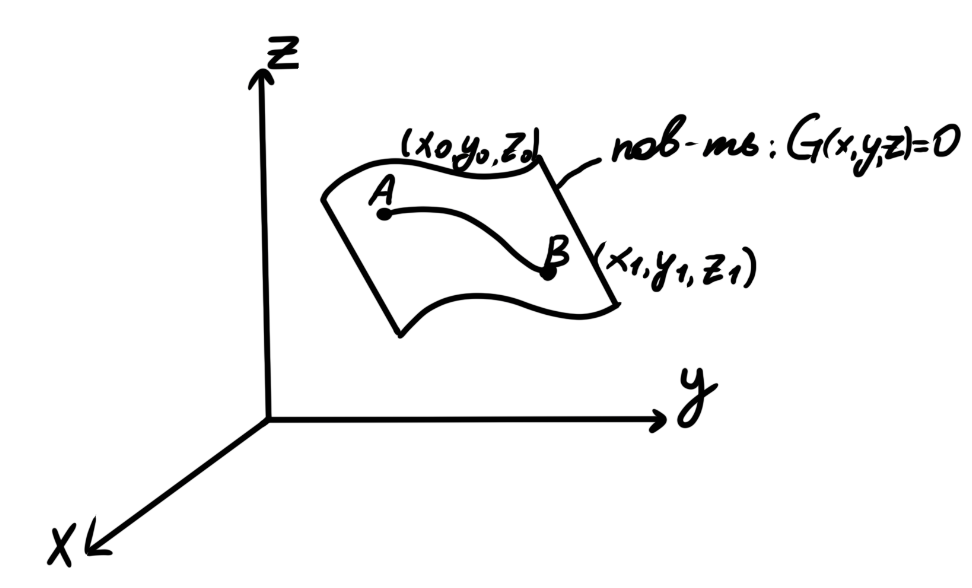
\includegraphics[width=0.5\textwidth]{/Users/vladbelousov/Desktop/Semestr_4-FP-NSU/ДфУ/Лекции_по_дням/image/19.png}
\end{center}

Найти кривую, соединяющую точки A и B, лежащие на поверхности, имеющую наименьшую длину. 

\[ \begin{cases}
x = x(t ) \\
y = y(t ) \quad  \text{уравнение кривой в параметрическом виде } ,\text{ }  t \in [t_0 , t_1]\\
z = z(t )
\end{cases} \] 

\[ I [x,y,z]  = \int_{t_0}^{t_1} \sqrt{(x' (t )) ^2 + (y' (t )) ^2 + (z' (t )) ^2 }dt \] 

\[\begin{cases}
x(t_0 ) = x_0 ,\quad x(t_1 ) = x_1 \\
y(t_0 ) = y_0 ,\quad y(t_1 ) = y_1 \\
z(t_0 ) = z_0 ,\quad z(t_1 ) = z_1
\end{cases} \] 

\textbf{Необходимое условие локального экстремума}:

Пусть \( \tilde{y_1 }, ..., \tilde{y }_n  \)  доставляют локальному экстремум для задачи (1). Тогда \( \exists    \lambda(t)   \) такая, что функции \( \tilde{y_1 }, ..., \tilde{y }_n  \) являются экстремалями вспомогательного функционала. 

\[ \tilde{I } [y_1, \ldots, y_n ] = \int_{t_0}^{t_1} (F + \lambda G(t))dt  \] 

\textbf{Без доказательства.} 

\section{Решение задачи о геодезических на сфере}

\begin{center}
    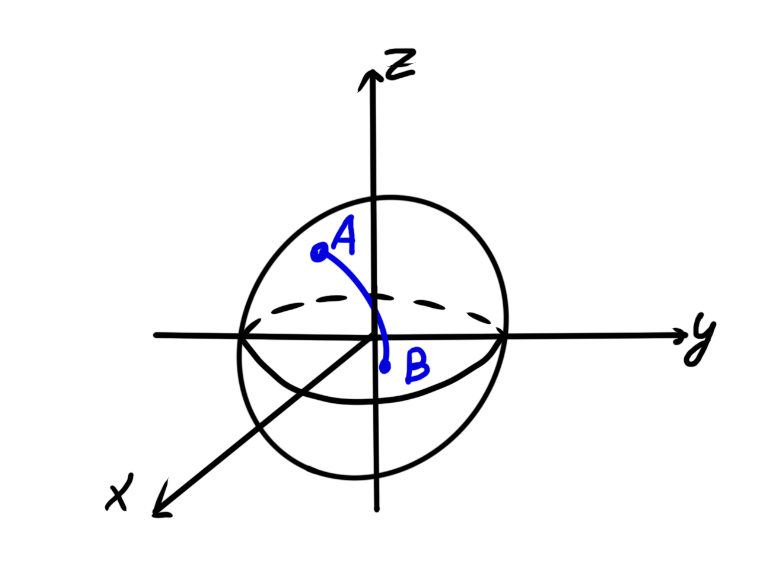
\includegraphics[width=0.4\textwidth]{/Users/vladbelousov/Desktop/Semestr_4-FP-NSU/ДфУ/Лекции_по_дням/image/20.png}
\end{center}

\[ x ^2  +y ^2 + z ^2 = R ^2  \] 

\[ I [x,y,z] = \int_{t_0}^{t_1} \sqrt{(x' (t )) ^2 + (y' (t )) ^2 + (z' (t )) ^2 }dt \] 

\[ \tilde{I } [x,y ,z ] = \int _{t_0}^{t_1}  \underbrace{\left(  \underbrace{\sqrt{(x' (t )) ^2 + (y' (t )) ^2 + (z' (t )) ^2 }}_{F}  + \lambda(t)(x ^2  +y ^2 + z ^2 - R ^2 ) \right)}_{\tilde{F}}  dt  \] 

\[\begin{cases}
    \displaystyle 2 x \lambda (t ) = \frac{d}{dt } \left( \frac{x' }{F}  \right) \quad (1)   \\
    \displaystyle 2 y \lambda (t ) = \frac{d}{dt } \left( \frac{y' }{F}  \right)  \quad (2)\\
    \displaystyle 2 z \lambda (t ) = \frac{d}{dt } \left( \frac{z' }{F}  \right) \quad (3)
\end{cases} \] 

\[ \begin{cases}
    \displaystyle (1) \cdot y + (2) \cdot (-x):\quad  y \frac{d}{dt } \left( \frac{x' }{F} \right) -x \frac{d}{dt } \left( \frac{y' }{F} \right) = 0 \\
    \displaystyle (2) \cdot z + (3 ) \cdot (- y) :\quad z \frac{d}{dt } \left( \frac{y' }{F} \right) -y \frac{d}{dt } \left( \frac{z' }{F} \right) = 0 \\
    \displaystyle (3) \cdot (-x) + (1) \cdot  z : \quad z \frac{d}{dt } \left( \frac{x' }{F} \right) -x \frac{d}{dt } \left( \frac{z' }{F} \right) = 0 
\end{cases} \] 

\[ \frac{d}{dt } \left( y \frac{x ' }{F }  - x \frac{y '}{F}  \right) = \cancelto{0}{y ' \frac{x ' }{F }} + y \frac{d}{dt } \left( \frac{x' }{F}  \right) \cancelto{0}{- x ' \frac{y '}{F}} - x \frac{d}{dt } \left( \frac{y' }{F}  \right) \] 

\[
\begin{aligned}
    \begin{cases}
        \displaystyle \frac{d}{dt } \left( y \frac{x' }{F } - x \frac{y ' }{F}  \right) = 0 \\
        \displaystyle \frac{d}{dt } \left( z \frac{y' }{F } - y \frac{z' }{F}  \right) = 0 \\
        \displaystyle \frac{d}{dt } \left( z \frac{x' }{F } - x \frac{z ' }{F}  \right) = 0 
    \end{cases} 
    \begin{cases}
        \displaystyle \frac{y x' - x y ' }{F } = c_1  \quad (1)\\
        \displaystyle \frac{z y' - y z ' }{F } = c_2  \quad (2)\\ 
        \displaystyle \frac{z x' - x z ' }{F } = c_3 \quad (3)
    \end{cases}
\end{aligned}\] 



\[ (1 )  \cdot z + (2)\cdot x + (3 ) \cdot (-y) : \]

\[ \frac{1}{F} \left[ z(y x' - x y ' ) + x (z y' - y z ' ) - y(z x' - x z ' ) \right] = c_1 z + c_2 x -  c_3 y  \] 

\[ \begin{cases}
    c_1 z + c_2 x -  c_3 y =  0 - \text{плоскость проходящая через (0,0,0)} \\
    x ^2 + y ^2 + z ^2 = R ^2 
\end{cases}  \] 

\begin{center}
    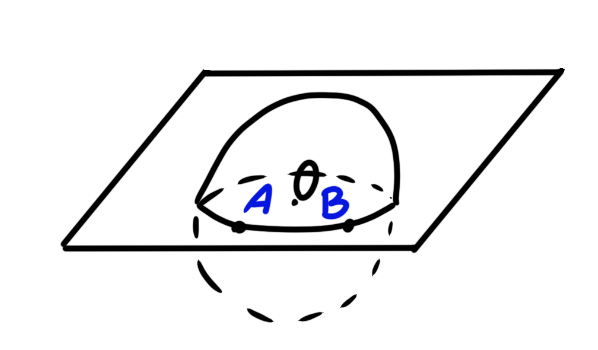
\includegraphics[width=0.3\textwidth]{/Users/vladbelousov/Desktop/Semestr_4-FP-NSU/ДфУ/Лекции_по_дням/image/21.png}
\end{center}

Геодезическая на сфере - дуга на большой окружности.

\chapter{Система малых колебаний}

\section{Линейные однородные системы малых колебаний}

\[ M \vec{x''}  + K \vec{x}  = 0  \quad  (1) \] 

\[ \vec{x }  =\vec{x } (t) = \begin{pmatrix}
x_1( t)\\
\vdots\\
x_n (t)
\end{pmatrix} \quad  M =\begin{pmatrix}
m_{11} & ... & m_{1n}\\
\vdots &  & \vdots\\
m_{n_1} & ... & m_{nn} 
\end{pmatrix} \quad K=\begin{pmatrix}
    k_{11} & ... & k_{1n}\\
    \vdots &  & \vdots\\
    k_{n_1} & ... & k_{nn} 
\end{pmatrix}  \]

Пример: \( n =1 \Rightarrow m x'' + kx = 0 , \text{ } m >0 , \text{ } k > 0 \) 

\begin{center}
    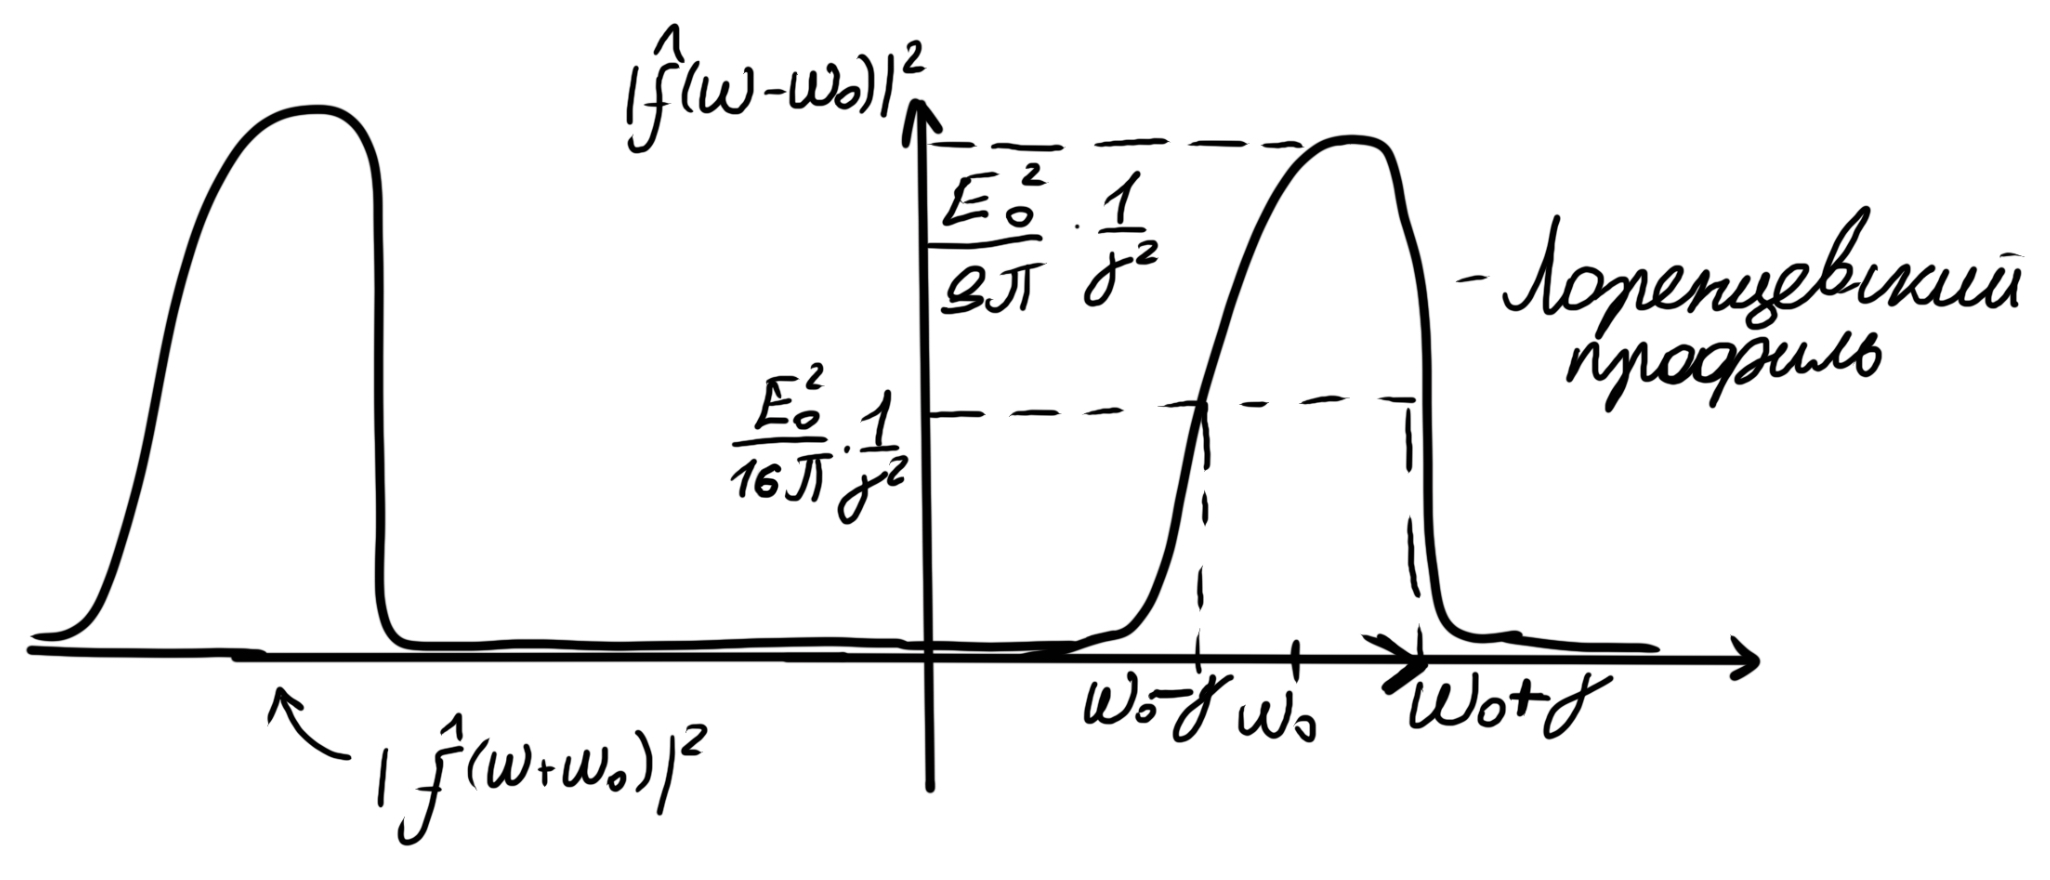
\includegraphics[width=0.3\textwidth]{/Users/vladbelousov/Desktop/Semestr_4-FP-NSU/ДфУ/Лекции_по_дням/image/22.png}
\end{center}

\[ M -\text{ матрица масс} , \quad  K -\text{ матрица жесткостей } \] 

1) \( M = M^{\top} , \text{ }  K = K^{\top}   \text{ } (m_{ij}= m_{j i} ,\text{ } k_{ij} = k_{j i}   ) \) 

2) M > 0  (матрица положительна определена), \( K \geq 0 \) 

\begin{definition}
    Матрица \( M = M^{\top} \) называется положительно определенной, если \( \forall \vec{v } \in  \mathbb{R} ^{n } , \vec{v } \neq 0  \) выполняется \( (M\vec{v} , \vec{v} ) >0 \).  
\end{definition}

\textbf{Критерий Сильвестра: } \( M = M^{\top} > 0 \Leftrightarrow  \text{все главные миноры} > 0. \)

\textbf{1-ый способ:} Сведение к системе 1-го порядка. 

\[ \begin{aligned}
    \begin{cases}
        \vec{y_1 } = \vec{x } \\
        \vec{y_2 } = \vec{x '} 
    \end{cases}
    \begin{cases}
        \vec{y_1 '} = \vec{y_2} \\
        \vec{y_2  '} = \vec{x ''} = -M ^{-1} K \vec{x }  = - M ^{-1} K \vec{y_1}   
    \end{cases}
\end{aligned} \] 

\[ \frac{d}{dt} \begin{pmatrix}
\vec{y_1} \\
\vec{y_2} \\
\end{pmatrix} = \underbrace{\overbrace{\begin{pmatrix}
    0 &  & E\\
     &  & \\
    -M^{-1}K  &  & 0
    \end{pmatrix}}^{A}}_{n \times n}  \begin{pmatrix}
\vec{y_1} \\
\vec{y_2} \\
\end{pmatrix}   \] 





\[ \begin{pmatrix}
    \vec{y_1} \\
    \vec{y_2} \\
\end{pmatrix} =\underbrace{e^{t A }}_{(2n \times  2n)} \underbrace{\vec{c}}_{(2n \times  1)}  = \begin{pmatrix}
\Phi_{11}(t) & \Phi_{12}(t)\\
\Phi_{12}(t) & \Phi_{22}(t)
\end{pmatrix} \begin{pmatrix}
\vec{c_1} \\
\vec{c_2} 
\end{pmatrix}  \]

\[ \vec{x} (t ) = \vec{y_1 } (t ) = F_{11} (t ) \vec{c_1 }  + F_{12} (t ) \vec{c_2 } \quad  (\text{2n констант} )    \] 

\begin{lemma}
    Если \( M = M^{\top} > 0  \), то \( \exists  M^{-1}  \)  
\end{lemma}

\begin{proof}
    \[  \] 
    Пусть не существует \( M^{-1} \Rightarrow \kern-30pt\underbrace{\mathrm{det } M = 0}_{\displaystyle \underset{ \displaystyle \det (M - 0 E) = 0}{\Rightarrow \lambda = 0 - \text{собств.знач.} }}\kern-30pt \Rightarrow \exists  \vec{v } \neq 0 : M \vec{v } = 0  \) 

    \[ (M\vec{v } , \vec{v }     ) = (0, \vec{v } ) = 0 - \text{  противоречие}  \] 
\end{proof}


\begin{proposition}[из алгебры]
    Пусть \( A = A^{\top} \Rightarrow  \)  все собственные числа \( \lambda_j \in  \mathbb{R}.  \) 

    Пусть  \( A = A^{\top} > 0 \Rightarrow  \) все собственные числа \( \lambda_j > 0.  \)
\end{proposition}

\begin{proposition}[из алгебры]
    Пусть \( A = A^{\top} \Rightarrow   \) в \( \mathbb{R} ^n  \)  существует базис из собственных векторов, то есть нет присоединенных 
\end{proposition}

\begin{proposition}[из алгебры]
    Пусть \( A = A^{\top} \Rightarrow A = U D U^{-1}  \), \( \begin{pmatrix}
    \lambda_1 &  & 0\\
    &\ddots  & \\
    0& & \lambda_n
    \end{pmatrix} \) 

\( U  \) - ортогональная  матрица, то есть \( U ^{-1} = U^{\top }   \)  
    
\end{proposition}

\textbf{2-ой способ:}

\begin{definition}
    Число \( \lambda     \)  называется собственным числом системы (1), если
    
    \( \det (K -\lambda M ) = 0 \) 
\end{definition}

\begin{definition}
    Вектор \( \vec{v }  \neq \vec{0}  \)  называется собственным вектором системы (1) (вектором нормальных колебаний), если \( (K -\lambda M ) \vec{v } = 0 \) 
\end{definition}

\begin{theorem}
    Существует n собственных чисел системы (1) и \( \lambda_{i } \geq 0 , \forall  i = 1,2,...,n \) 
\end{theorem}

\begin{proof}
\[  \]

1) \( \det (K -\lambda M )  = 0 \) 

\[ \det (M(M^{-1} K - \lambda E )) = 0 \] 

\[ \underbrace{\det M}_{ \neq 0} \det (M^{-1 } K - \lambda E ) = 0 \Rightarrow \text{ существует n собственных чисел}  \] 

2) \( \vec{v_j}  \)  - собственные вектора \( \Rightarrow K \vec{v_j} = \lambda_j M \vec{v_j} \text{ } | \cdot \vec{v_j}   \)  

\[ \underbrace{(K v_{j }  , v_j)}_{\geq 0}  = \lambda_j \underbrace{(M v_j ,v_j)}_{>0} \Rightarrow \lambda_j \geq 0  \] 
\end{proof}

\begin{theorem}
    В \( \mathbb{R} ^n \)  существует базис из собственных векторов системы (1).
\end{theorem}

\textbf{Доказательство будет позже.} 

\begin{theorem}
    Пусть  \( M = M^{\top} > 0 , K =K ^{\top} \geq 0 , \lambda_1, \ldots, \lambda_n \geq 0 \)  - собственные числа системы (1), \( \vec{v_1 },..., \vec{v_n}   \)  - собственные вектора системы (1), соответвующие числам \( \lambda_1, \ldots, \lambda_n \). Тогда все решения системы (1)  имеют вид: 

    \[ x(t) = \sum_{j=1} ^{n } q_j (t)\vec{v_j},   \] 

    , где \( q_j(t) \)  - решение дифференциального уравнения: \( q_j '' + \lambda_j q_j = 0 \) 
\end{theorem}

\begin{proof}
    \[  \] 
    По теореме 2 \( \vec{v_1},..., \vec{v_n }   \)  - базис в \( \mathbb{R} ^ n \). При фиксированном t \( x(t ) \in  \mathbb{R}^{n} \Rightarrow \vec{x } (t)  \)  раскладывается по базису: \( \vec{x } (t) = \sum_{j=1} ^{n } q_j (t)\vec{v_j}  \) 

    Подставляем \( x(t) \)  в систему (1): 

    \[ M \sum_{j =1}^n q_j '' (t ) \vec{v_j} + K \sum_{j =1}^n q_j (t ) \vec{v_j} = 0  \] 

    \[ \sum_{j=1}^ n \left( q_j '' (t ) M \vec{v_j } + q_j (t )\underbrace{ K \vec{v_j } }_{\lambda_j M \vec{v_j } } \right) =0\] 

    \[ \sum _{j=1}^ n \left( q_j '' (t ) M \vec{v_j } + \lambda_j q_j (t )M\vec{v_j }  \right) = 0 \text{ }  | \cdot  M^{-1}  \] 

    \[ \sum _{j=1}^ n \left( q_j '' (t  ) + \lambda_j q_j (t ) \right) \vec{v_j }= 0 , \text{ }  \forall  t \in  \mathbb{R}   \] 

    \[ \text{Т.к } \vec{v_1 },..., \vec{v_n} \text{ линейно независимы, то }  q_j '' (t ) + \lambda_j q_j (t) =0    \] 


\end{proof}

\begin{center}
    \textbf{Замечание.} \( q_j ''(t ) + \lambda_j q_j (t) = 0 \) 
    1) \( \lambda_j = 0 \Rightarrow q_j (t ) = c_1 t + c_2  \) 

    2) \( \lambda_j > 0 \Rightarrow q_j (t )  = c_1 \cos (\sqrt{\lambda_j} t) + c_2 \sin (\sqrt{\lambda_j} t) \)
\end{center}

\begin{definition}
    \( \omega_1 = \sqrt{\lambda_1},..., \omega_n = \sqrt{\lambda_n} \) называется собственными частотами колебаний системы (1).
\end{definition}

%%-------------------------------%%

% Закрытие документа, если файл компилируется отдельно
\ifdefined\mainfile
    % Если это основной файл, не нужно заканчивать документ
\else
    \end{document}
\fi
%Март
% Условная компиляция для самостоятельной работы
\ifdefined\mainfile
    % Если это часть основного файла, не добавляем начало и конец документа
\else
    \documentclass[12pt, a4paper]{report}
    \usepackage{/Users/vladbelousov/Desktop/Semestr_4-FP-NSU/Настройка/library}
    \usepackage[utf8]{inputenc} % Подключение поддержки UTF-8
    \begin{document}
\fi

%%-------------------------------%%

\begin{proof}[Докозательство теоремы 2.]
    \[  \] 
    \[ M = M ^{ \top } > 0 \Rightarrow \underset{>0}{\lambda_1 (M )},..., \underset{>0}{\lambda_n (M )} - \text{ собственные числа матрицы }  M \] 

    \[ M = U \begin{pmatrix}
    \lambda_1 (M) &  & 0\\
     & \ddots & \\
    0 &  & \lambda_n(M)
    \end{pmatrix} U^{-1} , \text{ можно взять } U \text{ - ортогональную матрицу, то есть } U^{ -1} = U^{\top}    \] 


\[ \sqrt{M} = U \begin{pmatrix}
    \sqrt{\lambda_1 (M)} &  & 0\\
     & \ddots & \\
    0 &  & \sqrt{\lambda_n(M)}
    \end{pmatrix}  U^{-1} \] 

    \[ \sqrt{M} \sqrt{M}  =M\]

    Пусть \( \vec{v_j}   \) - собственный вектор: \( (K- \lambda_j M ) \vec{v_j } =\vec{0}   \) 

    \[ (K - \lambda_j \sqrt{M } E \sqrt{M }) \vec{v_j} = 0 \] 

    \[ \sqrt{M } (\underbrace{(\sqrt{M })^{-1} K (\sqrt{M})^{-1}}_{A} - \lambda_j E   ) \sqrt{M } \vec{v_j} = 0 \] 

    \[ \lambda_j - \text{ собственное число } A , \text{ }  \sqrt{ M } \vec{v_j } -\text{ собственный вектор  }  A \] 

    \[ A= A^{\top} , \quad  A^{\top } =\underbrace{ [(\sqrt{M } )^{-1} ]^{\top }}_{(\sqrt{M })^{-1} } \underbrace{K^{\top }}_{K} \underbrace{ [(\sqrt{M } )^{-1} ]^{\top }}_{(\sqrt{M })^{-1} }    \] 

    Из алгебры (утверждение 2.) в \( \mathbb{R}     ^{ n }  \) существует базис из собственных векторов матрицы \( A : \sqrt{M }\vec{v_1 },..., \sqrt{M } \vec{v_n}    \). Так как \( \det \sqrt{M } \neq ,  \)  то \( v_1, \ldots, v_n \) - базис \( \mathbb{R} ^n  \). 
    \[  \] 
\end{proof}
 

\section{Линейные неоднородные системы  малых колебаний}

\[ M\vec{x} ''+ K\vec{x}  = \vec{f } (t)  \quad  (1 )\] 

\[ \vec{x }  =\vec{x } (t) = \begin{pmatrix}
x_1( t)\\
\vdots\\
x_n (t)
\end{pmatrix} , \text{ }  M, K - (n \times n) , \text{ }  M= M^{\top } > 0 , K =K ^{\top } \geq  0 , \vec{f } (t) = \begin{pmatrix}
f_1(t)\\
\vdots\\
f_n(t)
\end{pmatrix}\] 

1-способ. Сведение к системы 1-го порядка 

2-способ. 

\begin{theorem}
    Пусть \( \lambda_1, \ldots, \lambda_n \) - собственные числа, то есть \( \det (K - \lambda_j M ) = 0 \), \( v_1, \ldots, v_n  \)  - собственные вектора, то есть \( (K - \lambda_j M )v _j = 0 \) 


\end{theorem} 

\begin{proof}
    \[  \] 
    Пусть \( \lambda_1 \neq \lambda_2  \). Тогда \(\kern-0.8cm \underbrace{(M v_1 ,v_2 )}_{v_1,v_2 - M  \text{ - ортогональны} } =  \underbrace{(K v_1 ,v_2 )}_{v_1,v_2 - K \text{ - ортогональны} }\kern-0.8cm  = 0 \)  

    \[ \begin{aligned}
        \begin{cases}
            K v_1 = \lambda_1 M v_1  | \cdot v_2 \\ 
            K v_2 = \lambda_2 M v_2  | \cdot v_1 \\ 
        \end{cases} 
        \begin{cases}
        (K v_1 , v_2 ) = \lambda_1 ( M v_1 , v_2 ) \\ 
        (K v_2, v_1 ) = \lambda_2 ( M v_2 , v_1 ) \\ 
        \end{cases}
    \end{aligned}\] 

    \[ (K \vec{v } _1 , \vec{v }_2   )  = (v_1, K^{\top } v_2) = (v_1, K v_2 ) = (K v_2 , v_1 )\] 

Вычитаем одно из другого: 

\[ 0 = \lambda_1 (M v_1 ,v_2 ) - \lambda_2 (M v_2 , v_1  ) = \underbrace{(\lambda_1 - \lambda_2 )}_{\neq 0} (M v_1 ,v_2 ) \Rightarrow (Mv1, v_2 ) = 0 \Rightarrow (K v_1 ,v_2 ) = 0 \] 

\end{proof}

\begin{theorem}
    Пусть \( \lambda_1=, \ldots, =\lambda_p \) - собственное число кратности \( p \). Тогда существует собственные вектора \( \vec{w_1} , \ldots,\vec{w } _{p}   \), которые являются \( M  \)   - ортогональными, то есть \( (M w_i, w_j ) = 0  \) при \( i \neq j \) 
\end{theorem}


\begin{proof}

\[  \] 
    Из параграфа 1 (теорема 2) мы знаем, что \( \exists  \vec{v } _1 ,..., \vec{v } _p  \) - линейно независимые собственные вектора. 
    
    Метод \( M \) - ортогонализации Грама-Шмидта: 

    \[\vec{w_1 } = \vec{v_1 }    \] 

    \[ \vec{w_2 } = \vec{v_2 } + \alpha \vec{v_1 } , \text{ }  \alpha - ? , \text{  } ( M \vec{w_2 }, \vec{w_1 }  ) = 0    \] 

    \[ \underbrace{(M \vec{w_2 }, \vec{w_1}  ) }_{0}= (M\vec{v_2 }, \vec{w_1 }  ) + \alpha (M \underset{=\vec{w_1}}{\vec{v_1 }}, \vec{w_1}   )  \Rightarrow \alpha = \frac{ (M \vec{v_2 }, \vec{w_1}  )}{(M \vec{w_1 }, \vec{w_1}  )} \] 

    Пусть \( \vec{w_1 },..., \vec{w_{m-1} }    \) построены, причем \( (M \vec{w_i } , \vec{w_j}  )= 0 ,\text{ } i \neq j , \text{ } i,j= 1, \ldots, m-1 \) 

    \[ \vec{w_n } = \vec{v_m }+ \sum_{j =1}^{m -1 }  \beta_j \vec{w_j } , \text{ } \beta_j -? , \text{ } (M \vec{w_m }, \vec{w_i}  ) = 0, \text{ } i=1, \ldots, m-1    \]
    
    \[ \underbrace{(M \vec{w_m } , \vec{w_i }  )}_{0} = (M \vec{v_m }, \vec{w_i} ) +\underbrace{ \sum_{j =1}^{m-1 } \beta_j (M\vec{w_j }, \vec{w_i}  )}_{\beta_i \underbrace{(M\vec{w_i }, \vec{w_i }  )}_{>0}}  \] 

    \[ \Rightarrow \beta_i = \frac{ - (M \vec{v_m }, \vec{w_i }  )}{(M \vec{w_i }, \vec{w_i}  )}  ,\text{ }  j= 1, \ldots, m-1  \Rightarrow \vec{w_1 },.., \vec{w_p} \text{ - M-ортогональны}   \] 
\end{proof}

\begin{theorem}
    Пусть \( \lambda_1, \ldots, \lambda_n \)  - собственные числа системы (1), \( \vec{w_1 }, ,..., \vec{w_n}   \) - собственные вектора, которые М-ортогональны. Тогда решение (1) имеет вид: 

    \[ \vec{x } (t ) = \sum_{j =1}^{n } q_j \vec{w_j }  \] 

    \(\text{, где }  q_j (t ) \text{ - решение дифференциального уравнения: }  q_j '' + \lambda_j q_j = \tilde{f_j }(t) \) 
\end{theorem}

\begin{proof}
\[  \] 

    Так как \( \vec{w_1 },..., \vec{w_n }    \)  - базис в \( \displaystyle \mathbb{R}    ^n , \text{ } \vec{x } ( t  ) \in \mathbb{R} ^ n \Rightarrow \vec{x } (t ) = \sum_{j =1}^ n q_j ( t ) \vec{w_j } - \text{ решение (1)}. \) 

    \[ M \sum_{j =1}^ n q_j '' (t ) \vec{w_j } + \underbrace{K \sum_{j =1}^ n q_j (t ) \vec{w_j }}_{K \vec{w_j }= \lambda_j M \vec{w_j}  } = \vec{f } (t )   \] 

    \[ \sum_{j =1}^ n (q_j ''(t )+ \lambda_j q_j (t ))M \vec{w_j } = \vec{f } (t )  | \cdot \vec{w_i}   \] 

    \[ \sum_{j =1}^ n (q_j '' (t )+ \lambda_j q_j (t ))\underbrace{(M\vec{w_j }, \vec{w_i }  )}_{\tiny\begin{aligned}
    =0 , \text{ если } j\neq i \\
    \neq 0, \text{ если } j = i  
    \end{aligned}} = (\vec{f } (t ), \vec{w_i} ) \] 

    \[ (q_i '' (t ) + \lambda_i q_i (t ))(M \vec{w_i},  \vec{w_i }  )= (\vec{f } (t) , \vec{w_i} ) \] 

\end{proof}

\chapter{Зависимость решения от параметров}

\section{Непрерывная зависимость решений от параметров и начальных данных}

\[ \begin{cases}
    y ' =  f (t,y ) , \quad  f : \mathbb{D} \to  \mathbb{R} , \text{ } \mathbb{D} \subset \mathbb{R} ^2 , \text{ } \mathbb{D} \text{ - решение открытое}  \\ 
    y(t_0) = y_0
\end{cases} \] 


\begin{theorem}[Теорама Пикара]
    Если \( f \in  C(\mathbb{D} ) , \text{  } \exists  \frac{\partial  f }{\partial  y } \in  C(\mathbb{D} ) \Rightarrow \forall  (t_0, y_0 ) \in  D \text{ } \exists !    \)  непродолжаемое  решение задачи Коши, определенной на открытом интервале \( \alpha, \omega \) 
\end{theorem}

Будем менять \( y_0 \)

Решение задачи Коши: \( y (t; y_0) \) 

\begin{center}
    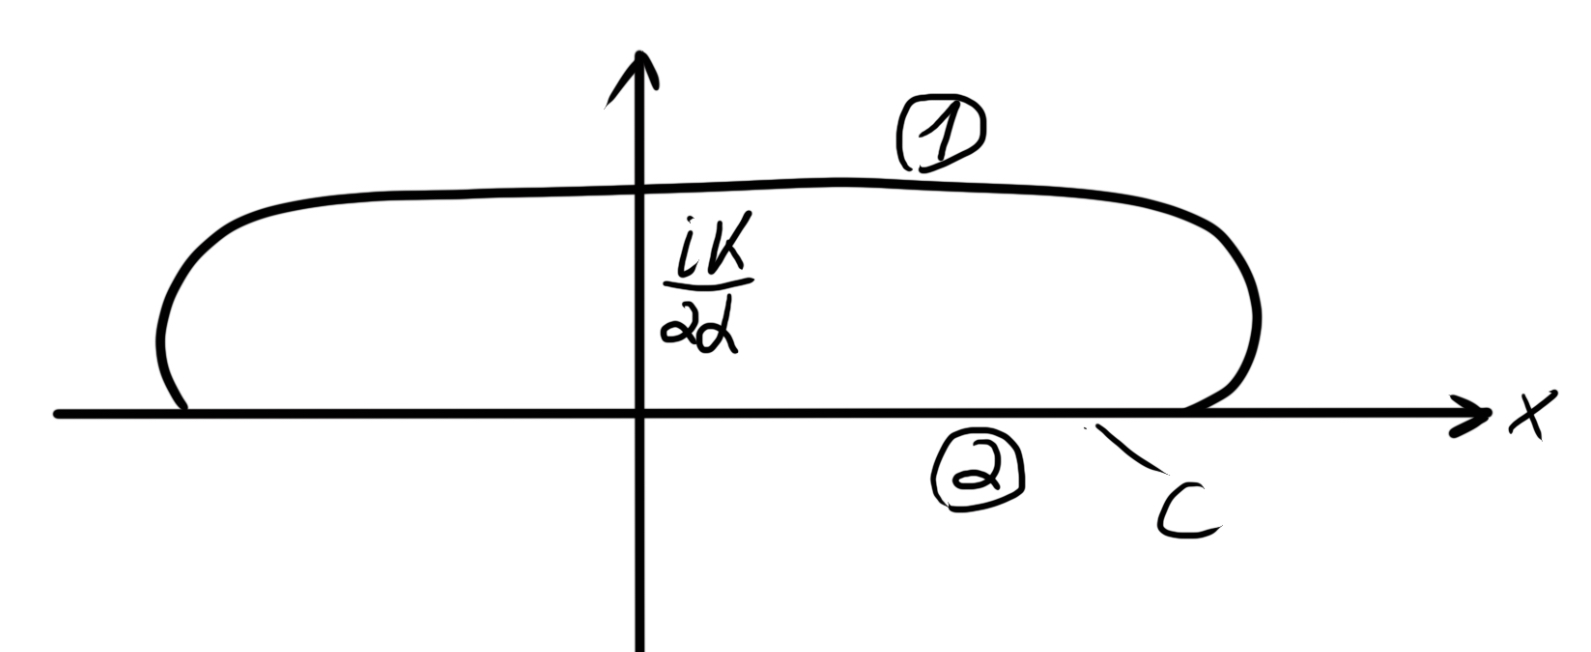
\includegraphics[width=0.5\textwidth]{/Users/vladbelousov/Desktop/Semestr_4-FP-NSU/ДфУ/Лекции_по_дням/image/23.png}
\end{center}

Вопрос: если \( y_0 \approx y_0^* \), можно ли утверждать, что \( y(t, y_0 ^* ) \approx y (t, y_0) \) 

Пример: 

\[ \begin{aligned}
    \begin{aligned}
        &\begin{cases}
            y ' = y ^2  \\ 
            y(0 ) = y^* = 0 
        \end{cases} \\
        &y(t, 0 )=0 , \text{ } t \in (-\infty , +\infty )
    \end{aligned}
    \quad \quad  
    \begin{aligned}
        &\begin{cases}
            y ' = y ^2 \\
            y(0) = y_0 > 0
        \end{cases} \\
        &y(t,y_0) = \frac{1 }{\frac{1}{y_0 } -t } , \text{ } t \in  \left( -\infty , \frac{1}{y_0}  \right)
    \end{aligned}
\end{aligned} \] 

\begin{theorem}
    Пусть \( f \in C(\mathbb{D}) , \text{ } \exists \frac{\partial f}{\partial y} \in C(\mathbb{D}) \). Пусть \((t_0, y_0^*) \in \mathbb{D}\). Пусть \( y(t, y_0^*) \) - решение задачи Коши, определенное на интервале \( (\alpha, \omega) \). Возьмем \( [t_1, t_2] \subset (\alpha, \omega) \). Тогда:

    1) \( \exists \Delta > 0 , \text{ }  \forall  y_0 : \left\lvert y_0 - y_0 ^*  \right\rvert < \Delta \Rightarrow y(t, y_0)\)  определенно при \( t \in  [t_1, t_2 ] \); 
    
    2) \( y(t, y_0 ) \xrightarrow{y_0 \to  y_0^* } y(t, y_0^*) , \text{ }  t \in [t_1, t_2 ]  \)
\end{theorem}

Пример: 

\[ (t_0, y_0 ^* ) = (0,0 ) \Rightarrow y (t, y_0 ^* ) \equiv 0 , \text{ } (\alpha , \omega ) = (-\infty , + \infty  ). \text{ Возьмем: } [-T, T]  \] 

\begin{center}
    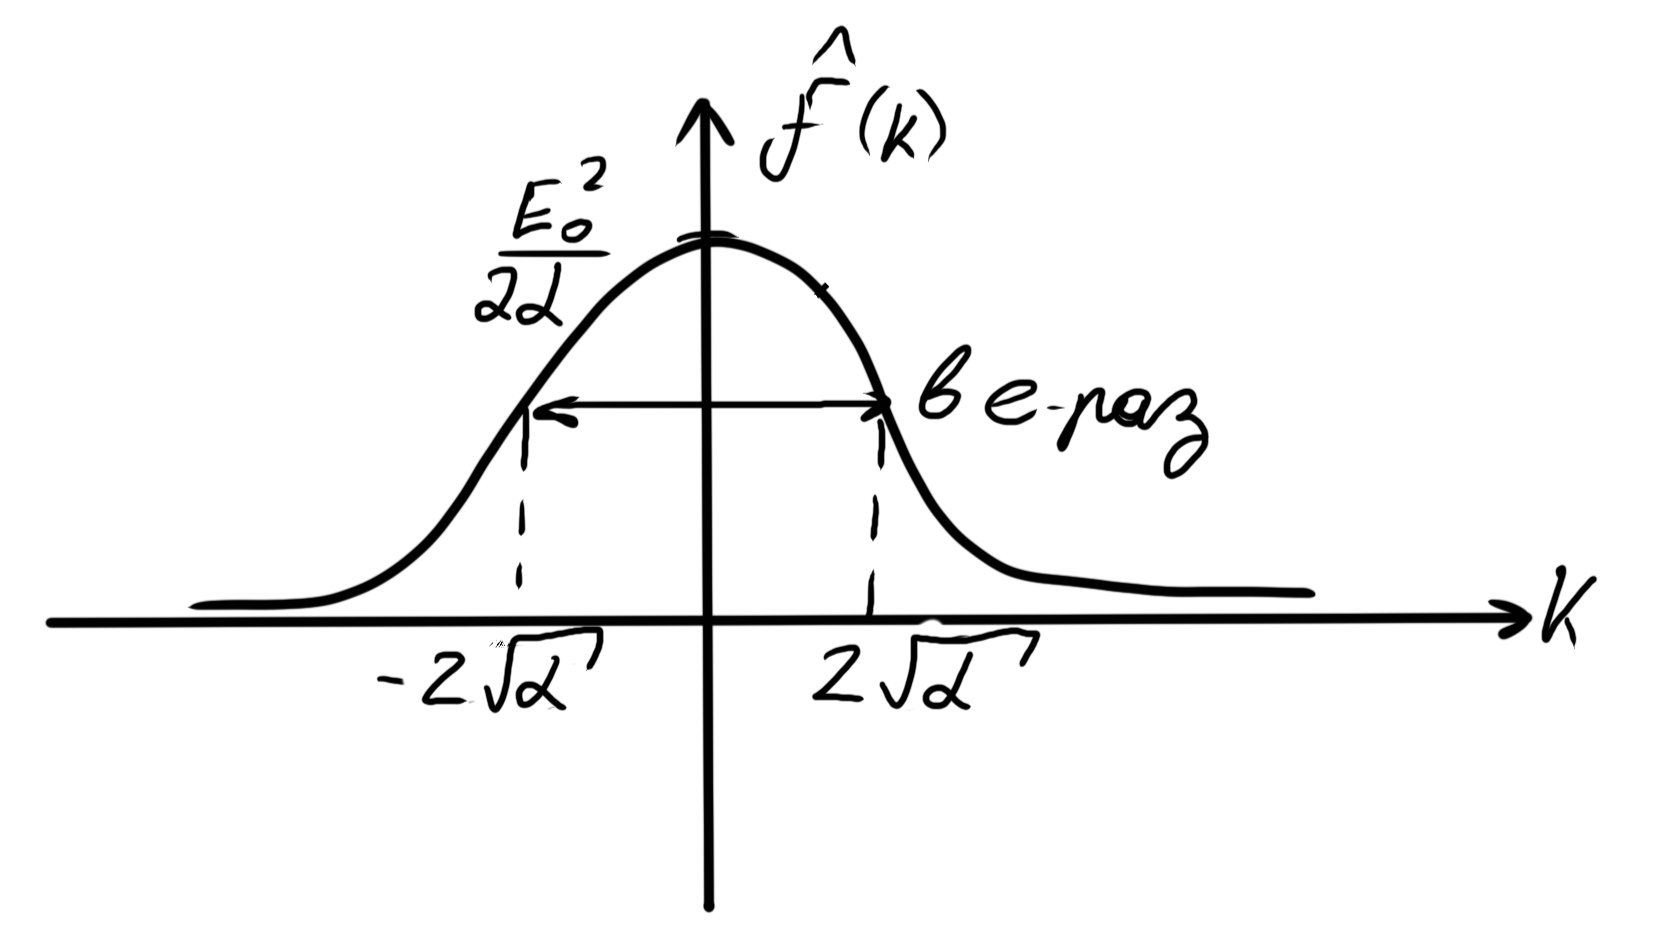
\includegraphics[width=0.4\textwidth]{/Users/vladbelousov/Desktop/Semestr_4-FP-NSU/ДфУ/Лекции_по_дням/image/24.png}
\end{center} 
\[ 1) \text{ } y_0 > 0 ;\text{ }  T < \frac{1}{y_0 } \Leftrightarrow y_0 < \frac{1}{T } =\Delta  \] 

\[ 2) \text{ } y(t,y_0 )= \frac{1}{\frac{1}{y_0 } - y    } \xrightarrow{y_0 \to  0 } 0 , \text{  }  t \in [-T,T]    \] 

%%-------------------------------%%

% Закрытие документа, если файл компилируется отдельно
\ifdefined\mainfile
    % Если это основной файл, не нужно заканчивать документ
\else
    \end{document}
\fi
% Условная компиляция для самостоятельной работы
\ifdefined\mainfile
    % Если это часть основного файла, не добавляем начало и конец документа
\else
    \documentclass[12pt, a4paper]{report}
    \usepackage{/Users/vladbelousov/Desktop/Semestr_4-FP-NSU/Настройка/library}
    \usepackage[utf8]{inputenc} % Подключение поддержки UTF-8
    \begin{document}
\fi

%%-------------------------------%%
\[ f: \mathbb{D} \to  \mathbb{R}     , \text{ } \mathbb{D} \subset \mathbb{R} ^2  , \text{ } \mathbb{D} \text{ - непустое открытое множество} \] 

Зависимость от параметра: 

\[ \begin{aligned}
    \begin{cases}
        y ' = f(t, y , \mu^* ) \\
        y(t_0 )= y_0
        \end{cases}
        \quad  \Rightarrow \quad 
        y(t, \mu^* ) \text{ - решение } 
\end{aligned} \] 

\[ \begin{aligned}
    \begin{cases}
        y ' = f(t , y , \mu ) \\
        y(t_0 )= y_0
        \end{cases} 
        \quad \Rightarrow \quad      
        y(t, \mu )  \text{ - решение } 
\end{aligned}\]

\begin{center}
    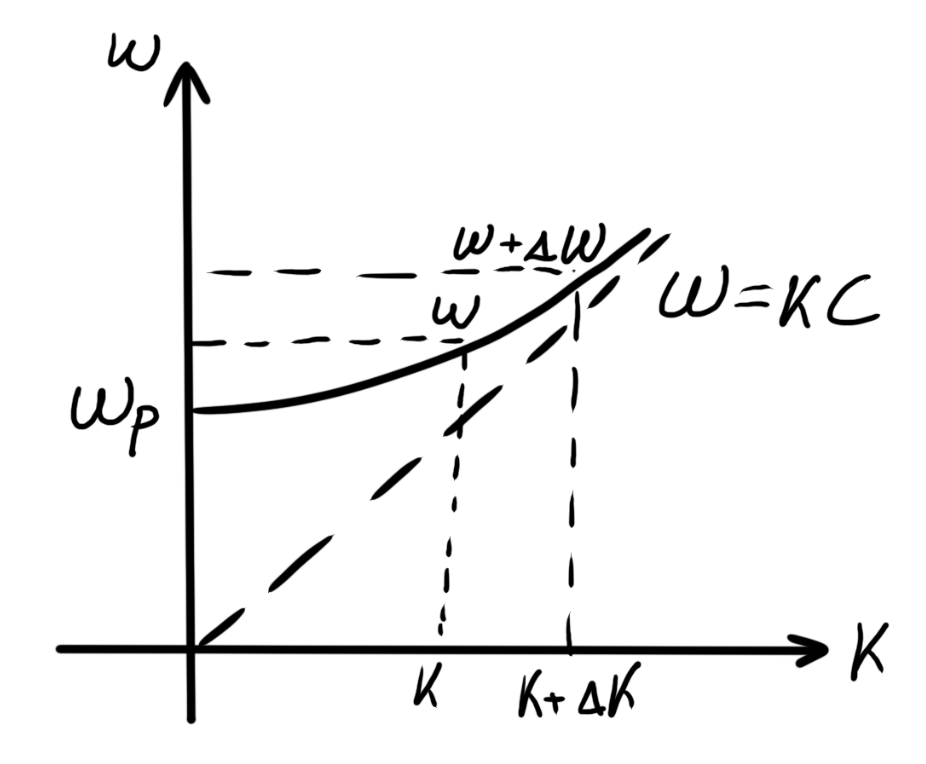
\includegraphics[width=0.4\textwidth]{/Users/vladbelousov/Desktop/Semestr_4-FP-NSU/ДфУ/Лекции_по_дням/image/26.png}
\end{center}

Пример 2: 

\[ \begin{aligned}
    \begin{cases}
        y = \mu^{* }  y ^2 = 0 \cdot y ^2 \\
        y(0 ) = 1
        \end{cases} 
        \quad \Rightarrow \quad 
        y(t,0 ) =1
\end{aligned}\] 

\[ \begin{aligned}
    \begin{cases}
        y = \mu  y ^2 = 0 \cdot y ^2 \\
        y(0 ) = 1
        \end{cases} 
        \quad \Rightarrow \quad 
        y(t,\mu ) = \frac{1}{1 - \mu t } 
\end{aligned}\] 

\begin{center}
    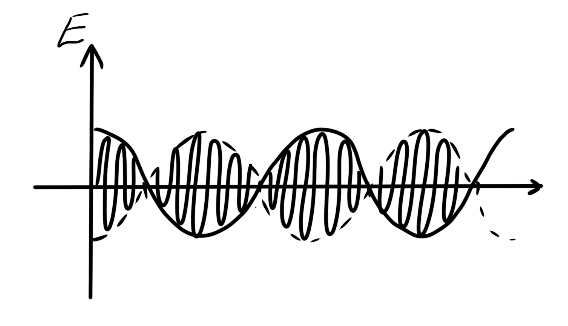
\includegraphics[width=0.5\textwidth]{/Users/vladbelousov/Desktop/Semestr_4-FP-NSU/ДфУ/Лекции_по_дням/image/27.png}
\end{center}

\begin{flushleft}
    \textbf{Теорема 2.} \textit{ \( f : B \to  \mathbb{R} , \text{ }  B \subset \mathbb{R} ^3 , \text{ } B  \) - непустое множество. Пусть  \( f \in  C(B ) \) \( \displaystyle  , \text{ } \exists  \frac{ \partial  f }{\partial  y } \in  C (B ) , \text{ }  (t_0, y_0 , \mu^* ) \in  B  \). Пусть \( y (t,\mu^* ) \) определено на  интервале \( (\alpha, \omega) \). Возьмем \( [t_1, t_2 ] \in  (\alpha , \omega) \)   }:  
    
    1) \( \exists  \Delta > 0 , \text{ }  \forall  \mu : |\mu - \mu^*   | < \Delta \Rightarrow y ( t, \mu ) \textit{ определено на } [t_1,t_2 ]  \) 

    2) \(  y(t,\mu ) \xrightarrow{\mu \to  \mu^* } y(t, \mu^*)   \text{ } \forall  t \in  [t_1,t_2 ]\) 
\end{flushleft}

Пример 2: 

\[ f(t, y ,\mu ) = \mu y ^2 , \text{ }  B = \mathbb{R} ^3 , \text{ }  f \in  C ( \mathbb{R} ^3 ) , \text{  } \exists  \frac{\partial  f }{\partial  y } \in  C (\mathbb{R} ^3 ) , \text{ }  ( 0,1,0 ) \in \mathbb{R} ^3   \] 

\[ y(t, \mu ^ * ) = y ( t, 0 ) = 1 , \text{ }  (\alpha , \omega ) = ( - \infty  , \infty ) \] 

Возьмем \( [-T, T ] \subset ( - \infty  , \infty  ) \) 

\begin{center}
    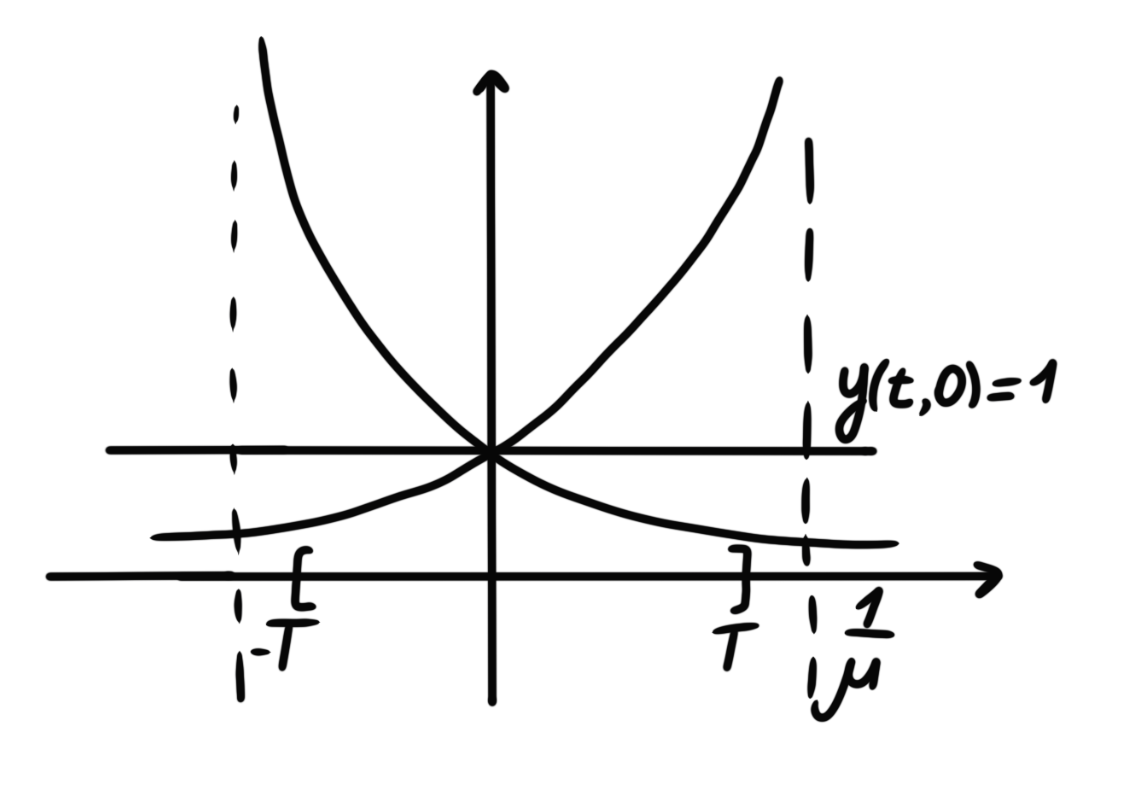
\includegraphics[width=0.5\textwidth]{/Users/vladbelousov/Desktop/Semestr_4-FP-NSU/ДфУ/Лекции_по_дням/image/28.png}
\end{center}

\[1) \text{ }  \mu > 0 : \frac{1}{\mu } > T \Leftrightarrow  \mu < \frac{1}{T  }  \quad  \mu < 0 : \frac{1}{\mu } < -T \Leftrightarrow \mu>  - \frac{1}{T }       \] 

\[ - \frac{1}{T }  < \mu < \frac{1}{ T }  \Leftrightarrow  |\mu     | < \frac{1}{T   } = \Delta   \] 

\[ 2) \text{ }  t \in [- T , T ] : \frac{1}{1 - \mu T } \xrightarrow{ \mu \to  0 } 1     \] 

\begin{proof}[Доказательство теоремы 1 с использованием теоремы 2]

    \[  \] 
    \[ \begin{aligned}
    \begin{cases}
    y ' = f(t ,y ) \\
    y (t_0 ) = y_0^ * 
    \end{cases}
    \quad  \Rightarrow \quad  y (t, y_0 ^*)
    \end{aligned} \] 
    
    \[ \begin{aligned}
        \begin{cases}
        y ' = f(t ,y ) \\
        y (t_0 ) = y_0
        \end{cases}
        \quad  \Rightarrow \quad  y (t, y_0)
        \end{aligned} \] 

        Замена переменных \( z(t, y_0 ) = y (t, t_0 ) - y_0 \) 

        \[ \begin{aligned}
        \begin{cases}
            y_t ' = z_y ' + (y_0  ' )_t  = z_t ' = f(t,y ) = f(t,z+ y_0) \\  
            z(t_0 ) = y(t_0  ) - y_0(t_0 ) = y_0 - y_0 = 0
        \end{cases}
        \end{aligned} \] 

        \[ \begin{aligned}
        \begin{cases}
            z_t ' = f(t , z+ y_0 ) \\ 
            z(t_0 )= 0 
        \end{cases}
        \text{ Замена: } y_0 = \mu
        \begin{cases}
        z_t ' = f(t, z+ \mu ) \\ 
        z(t_0 ) = 0
        \end{cases}  
        \quad \Rightarrow \quad  
        \end{aligned} \] 

        \[ \Rightarrow \text{ по теоремы 2 выполнено 1) и 2) } \Rightarrow \text{ выполнено 1) и 2) из теоремы 1 }   \] 
\end{proof}

\section{Дифференцируемость решений по параметрам и начальным данным}

\[ \begin{aligned}
\begin{cases}
y ' = f(t,y , \mu ) \\ 
y (t_0 )= y_0 
\end{cases}
\quad \Rightarrow \quad  
y(t, \mu) \, \text{ Хотим }: \exists  \frac{\partial  f }{\partial  y } 
\end{aligned} \] 

Пусть  \( \exists  \frac{\partial  y }{\partial \mu }  \) - непрерывна. Тогда по формуле Тейлора: 

\[ y(t, \mu ) = y(t, \mu^* ) + \frac{\partial  }{\partial  \mu } y(t,\mu ^* ) (\mu - \mu^* ) +\underbrace{ g (t, \mu )}_{o(\mu - \mu^*)} , \quad  \lim_{\mu  \to \mu^ * } \frac{ g(t, \mu )}{\mu - \mu^* } = 0   \] 

\[ f: B \to  \mathbb{R} , \text{ }  B \subset \mathbb{R}    ^3  , \text{ }  B \text{ - непустое открытое множество}  \] 

\begin{theorem} [Теорема 3.]
    Пусть \(  f \in  C (B ) , \text{ }  \exists  \frac{\partial  f }{\partial  y } \in  C (B ) , \text{  } \exists  \frac{\partial  f }{\partial  \mu } \in  C (B )     \). Пусть \( (t_0 , y_0 , \mu^* ) \in  B   , y(t, \mu ^* )   \)  определено на \( (\alpha , \omega ) \). Возьмем \( [t_1,t_2 ] \in (\alpha , \omega ) \). Тогда: 
    
    0) \( \displaystyle  \exists  \Delta > 0 , \text{ }  \forall  \mu : |\mu - \mu^*    |  < \Delta \Rightarrow y( t, \mu )\) определено на \( [ t_1,t_2 ] \) 

    1) \(\displaystyle  \exists  \frac{\partial  y }{\partial  \mu } (t, \mu) \in  C (P) ,  \) где \( P= \{(t,\mu ): t \in  [t_1, t_2 ] , \text{ } |\mu - \mu^* | < \Delta \} \) 

    2) \( \displaystyle  \exists  \frac{\partial  ^2 y } {\partial  \mu \partial  t } \in  C ( P)  \) 

    3) \( \underbrace{v ( t ,\mu )}_{\frac{\partial  y }{\partial  \mu }(t,\mu ) } \) - решение задачи Коши: \( \begin{cases}
    \displaystyle \frac{\partial  }{\partial  t } v = \frac{\partial  f } {\partial  y } + \frac{\partial  f }{\partial  \mu } \xleftarrow{ }  \text{ уравнение в вариациях Пуанкаре}  \\ 
    v(t_0 )  = 0   
    \end{cases} \) 
\end{theorem}

Пример 3: 

Найти решение \( y (y , \mu ) \)  при \( \mu  \), близких к нулю.

\[ \begin{aligned}
    \begin{cases}
        y ' = 4t \mu - y ^2 \\ 
        y (1 ) = 1 
        \end{cases}
        \quad \Rightarrow \quad  
        y(t , \mu)
\end{aligned} \] 

\[ \mu = \mu^ * = 0 , \quad  \begin{aligned}
    \begin{cases}
        y ' = - y ^2  \\ 
        y(1 ) =1 
        \end{cases} 
        \quad  y(t , 0 ) = \frac{1}{ t }  , \text{ } t \in  \underbrace{( 0, + \infty  )}_{(\alpha , \omega)}
\end{aligned} \] 

\[ f ( t ,y ,\mu ) = 4 t \mu - y ^2 , \text{ }  B =\mathbb{R} ^3  \] 

\begin{center}
    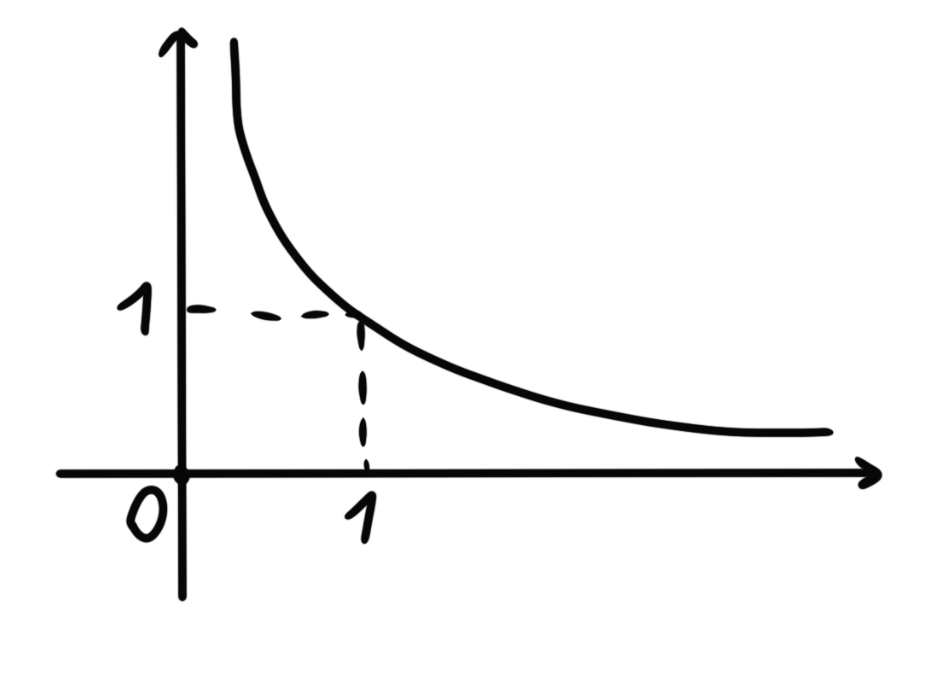
\includegraphics[width=0.5\textwidth]{/Users/vladbelousov/Desktop/Semestr_4-FP-NSU/ДфУ/Лекции_по_дням/image/29.png}
\end{center}

\[ f  \in  C (B ) , \text{ } \exists  \frac{\partial  f }{\partial y  }  \in  C (B ) , \text{ }  \exists  \frac{\partial  f }{\partial  \mu} \in  C ( \mathbb{R} ) , \text{ }  (1, 1, 0 ) \in \mathbb{R} ^3 \] 

Возьмем  \( [ t_1, t_2 ] \subset (  0, + \infty  ) \) 

\[ \Rightarrow 0 ) \exists  \Delta > 0 :  \forall \mu    : |\mu| < \Delta \Rightarrow y(t, \mu ) \text{ - определено на } [t_1,t_2 ]   \] 

\[ \Rightarrow 1) \exists  \frac{\partial  y }{\partial  \mu } ( t, \mu ) \in  C ( P )  \] 

\[ \Rightarrow y(t, \mu ) = \underbrace{y ( t, 0 )}_{\frac{1}{t  } } + \frac{\partial  y } {\partial  \mu } (t ,0 ) \mu    + o( \mu ) , \text{ } t \in  [t_1,t_2 ]  \] 

\[ \begin{cases}
    \frac{\partial  }{\partial  t } y ( t, \mu ) = 4 t \mu - y ^2 ( t, \mu )  \\
    y ( t ,\mu)  |_{t =1 }  =1 
\end{cases} \] 

Дифференцируем по \( \mu  \): 

\[ \begin{cases}
    \displaystyle \frac{\partial  }{\partial  \mu } \frac{\partial  }{\partial  t } y(t ,\mu ) = 4 t - 2 y(t,\mu)   \cdot \frac{\partial  y }{\partial  \mu }(t,\mu ) \\
    \displaystyle \frac{\partial  }{\partial  \mu } y (t,\mu ) |_{t =1 }  =0 
\end{cases} \] 

\[ \begin{cases}
\displaystyle \frac{\partial  }{\partial  t } \underbrace{\frac{\partial  y }{\partial  \mu } (t ,\mu )}_{ v(t, \mu)} = 4 t - 2 y ( t, \mu ) \cdot \underbrace{\frac{\partial  y }{\partial  \mu } (t ,\mu )}_{ v(t, \mu)}   \\
\displaystyle \underbrace{\frac{\partial  y }{\partial  \mu } (t ,\mu )}_{ v(t, \mu)}|_{t =1 }  =0 
\end{cases} \] 

\[ \mu = 0 : \text{ Обозначим } w (t ) = \frac{\partial  y } {\partial  \mu } (t , \mu ) |_{\mu =0}    \] 

\[\begin{aligned}
    \begin{cases}
        \displaystyle \frac{\partial  }{\partial  t }w (t ) = 4 t - 2 y (t, 0 ) w (t ) \\ 
        w(t ) |_{t =1} = 0  
    \end{cases}
    \begin{cases}
    \displaystyle w' = 4 t - \frac{2}{t }  w \\ 
    w(1 ) = 0
    \end{cases}
\end{aligned} \] 

1) Ищем решение однородного уравнения: 

\[ \displaystyle w ' = -\frac{2}{t } w \Rightarrow  w  =  \frac{c}{t ^2 }  \]

2) Ищем частное решение: 

\[ \displaystyle  w( t ) = \frac{ u (t )}{t ^2 }   \] 

\[ \frac{ u ' (t )}{t ^2 } - \frac{ 2 u(t )}{t ^3} = 4 t - \frac{2}{t }  \frac{u (t )}{t ^2 } \Rightarrow u'(t ) = 4 t ^3    \] 

\[ u(t ) = t ^4 + \tilde{c }\] 

3) Общее решение неоднородного уравнения: 

\[ w(t ) =  \frac{ t ^{ 4 }  + c }{t ^2 } = \frac{ t ^{ 4 } -1       }{ t ^2 }   \] 

\[ \Rightarrow y (t ,\mu ) = \frac{1}{t } + \frac{ t ^ 4 - 1 }{t ^2 } \mu + o(\mu ) , \text{ }  t \in  [t_1 ,t_2 ] \subset (0, + \infty  ) , \text{ }  |\mu     |< \Delta   \] 

\[ \begin{aligned}
    \begin{cases}
        y ' = f(t, y ) \\ 
        y(t_0 )= y_0 
        \end{cases} 
        \quad \Rightarrow \quad  y (t, y_0 )
\end{aligned} \] 

\[ f: \mathbb{D} \to  \mathbb{R} , \text{ }  \mathbb{D} \subset \mathbb{R} ^2 , \text{ }  \mathbb{D} \text{  - непустое открытое множество}  \] 

\begin{theorem}(Теорема 4.)
    Пусть \( f \in  C (\mathbb{D} ) , \text{ } \exists \frac{\partial  f }{\partial  y } \in  C(\mathbb{D} )   \). Пусть \( (t_0 , y_0 ^* ) \in  \mathbb{D} , \text{  } y(t ,y_0^* ) \) определено на \( (\alpha , \omega ) \). Возьмем \( [t_1,t_2 ] \subset (\alpha \omega ) \). Тогда: 
    
    0) \( \exists  \Delta > 0 , \text{ } \forall  y_0 : |y_0 - y_0 ^* | < \Delta \Rightarrow y(t, y_0 )  \)  определено на \( (\alpha , \omega) \) 

    1) \( \exists \frac{\partial  y }{\partial  y_0 } \in  C (P )  \), где \( P = \{(t, y_0 ): t \in  [t_1 ,t_2 ] , \text{ } |y_0 - y_0 ^* < \Delta|\} \)  

    2) \( \exists  \frac{\partial  ^2 y }{\partial  \mu \partial  t }  = \frac{\partial  ^2 y }{\partial  y_0 \partial  t_0 } \in C(P) \) 

    3) \( v(t, y_0 ) = \frac{\partial  y }{\partial  y_0 } (t,y_0 )   \)  -решение задачи Коши \( \begin{cases}
    \displaystyle \frac{\partial  }{\partial  t }v = \frac{\partial  f }{\partial  y } v  \\ 
    v (t_0 ) =1   
    \end{cases} \) 
\end{theorem}





%%-------------------------------%%

% Закрытие документа, если файл компилируется отдельно
\ifdefined\mainfile
    % Если это основной файл, не нужно заканчивать документ
\else
    \end{document}
\fi
% Условная компиляция для самостоятельной работы
\ifdefined\mainfile
    % Если это часть основного файла, не добавляем начало и конец документа
\else
    \documentclass[12pt, a4paper]{report}
    \usepackage{/Users/vladbelousov/Desktop/Semestr_4-FP-NSU/Настройка/library}
    \usepackage[utf8]{inputenc} % Подключение поддержки UTF-8
    \begin{document}
\fi

%%-------------------------------%%

\chapter{Периодические решения}

\section{Периодические решения линейных систем}

\[ \frac{d}{dt } \vec{y }  = A(t ) \vec{y } + \vec{f } (t ) \quad  (1) \] 

\[ \vec{y}  (t ) =\begin{pmatrix}
y_1(t)\\
\vdots\\
y_n(t)
\end{pmatrix}  ,\quad  A(t ) = ( a_{ij }(t)  ) - (n \times  n) , \quad \vec{f} (t ) =\begin{pmatrix}
    f_1(t)\\
    \vdots\\
    f_n(t)
\end{pmatrix}  \] 
\[ a_{ij } (t ) \in C(\mathbb{R}) , \text{ } f_j (t ) \in  C(\mathbb{R} ) \Rightarrow \exists ! \text{ решение задачи Коши }  \begin{cases}
\displaystyle  \frac{d}{dt }  y = A (t ) y + f(t  ) \\
y(t_0 ) = t_0 
\end{cases} \]
\[ y(t )  \text{ - определенно при } t \in  \mathbb{R}\]   

\[ a_{ij }  (t+T      ) = a_{ij }  (t ) , \text{ }  \forall  t \in  \mathbb{R} , \text{ }  T > 0 \text{ - период}  \] 
\[ f_j (t + T ) = f_j(t)  \] 

Хотим узнать, существуют ли у системы (1) периодические решения, то есть \( \vec{y } (t+ T) = \vec{y } (t ) \).

\begin{theorem}
    Вектор функция \( \vec{y } (t ) \)  является \( T \)-периодическии решением системы (1) \( \Leftrightarrow  \vec{y } (0 ) = \vec{y }  (T)  \) 
\end{theorem}

\begin{proof} \(  \) 
    \begin{flushleft}
         \((\Rightarrow ): \text{ очевидно }  \)
    \end{flushleft}  

    \begin{flushleft}
        \( (\Leftarrow):  \) 
    \end{flushleft}

    Обозначим \( \vec{y } (0 )= \vec{y } (T )= \vec{y}  _0  \) 

    Рассмотрим задачу Коши \( \begin{aligned}
        \displaystyle \begin{cases}
            \displaystyle  \frac{d}{dt }  \vec{y }  = A(t ) \vec{y } + \vec{f }  (t)\\
            \vec{y } (0) = \vec{y } _0
            \end{cases}
            \quad \Rightarrow \exists  ! \text{ решение } \vec{y} (t ) 
    \end{aligned} \) 

    Рассмотрим функцию \( \vec{z } (t    ) = \vec{y } (t+T ) \) 

    \[ \begin{cases}
        \frac{d}{dt } \vec{z }  (t ) = \frac{d}{dt }  \vec{y }  (t +T) = \underbrace{A (t + T )}_{A(t )} \underbrace{\vec{y } (t+T )}_{\vec{z } (t )} +\underbrace{\vec{f }  (t + T )}_{\vec{f } (t )} \\
        \vec{z } (0) = \vec{y } (T ) = \vec{y } _0 
    \end{cases}\]  

\[  \text{, получим такую же задачу Коши}    \Rightarrow \vec{z } (t ) = \vec{y } (t ) \Rightarrow \vec{y } (t+T ) = \vec{y } (t)\] 
\end{proof}

\[ y ' = a(t ) y + f(t )\] 
\[ a(t +T ) = a(t ) \]  
\[ f(t+T ) = f(t )\]  

\begin{center}
    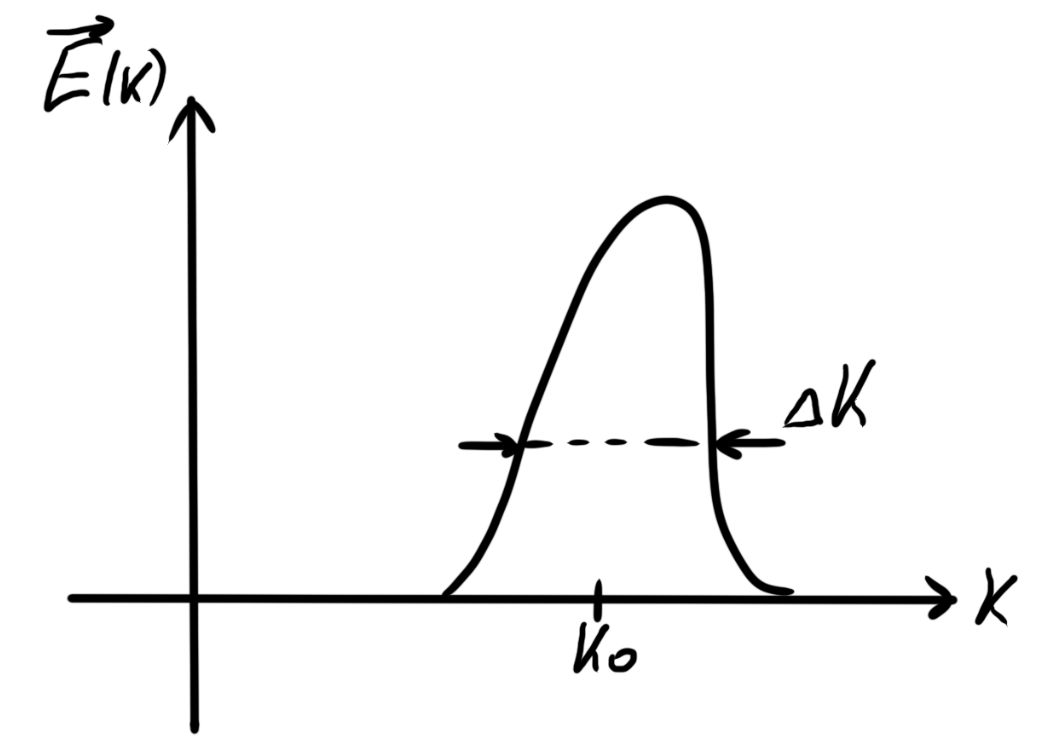
\includegraphics[width=0.4\textwidth]{/Users/vladbelousov/Desktop/Semestr_4-FP-NSU/ДфУ/Лекции_по_дням/image/30.png}
\end{center}

\begin{theorem}
    \( \exists !    \text{ }  T\)-периодическое решение системы (1) \( \Leftrightarrow  \det (\Phi (T ) - \Phi (0)) \neq 0  \), где \( \Phi(t) \) - ФМР системы \( \displaystyle  \frac{d}{dt } \vec{y } (t )= A(t )\vec{y} (t) \) 
\end{theorem}

\begin{proof}
    \begin{flushleft}
        Все решения системы \( \displaystyle  \vec{y }  (t) = \vec{ y } _{oo} (t )+ \vec{y } _{\text{ч} }(t ) = \Phi(t ) \vec{c }  + \Phi(t ) \cdot \int_{0}^{t }  \Phi^{-1 } (s ) \vec{f } (s )ds   \) 
    \end{flushleft}

    По теореме 1. : \( \vec{y } (0) = \vec{y } (T )  \):

    \[\Phi(0 ) \vec{c }  + \Phi(0 ) \int_{0 }^{0 } \Phi^{-1 } (s ) \vec{f } (s ) ds = \Phi(T ) \vec{c }  +\Phi(T ) \int_{0}^{T } \Phi^{-1 }  (s) \vec{f } (s ) ds  \] 

    \[\Phi ( 0) \vec{c } = \Phi (T ) \vec{c }  + \Phi (T ) \int_{0 }^{T }  \Phi^{-1 }  (s ) \vec{f } (s ) ds   \] 
    \[ (\Phi(0 )- \Phi(T ))\vec{c }  = \Phi(T ) \int_{0 }^{T } \Phi^{-1 } (s )\vec{f } (s )ds \Leftrightarrow  B \vec{c }  = \vec{\psi}  \]  

    \[ \exists ! \text{ } T\text{-периодическое решение  } \Leftrightarrow \exists ! \text{ }  \vec{c }  \Leftrightarrow  \det  (\Phi(0 )- \Phi(T )) \neq 0  \] 
\end{proof}

\begin{flushleft}
    \textbf{Замечание. } \textit{Если \( \det  B = \det  (\Phi(0 )- \Phi(T ))  = 0\), то}
    
    \textit{1) \( \rank B  = \rank  (B|\vec{\psi} ) \), то \( \exists \infty   \)  много \( T \)-периодических решений } 
    
    \textit{2) \( \rank B \neq  \rank (B|\vec{\psi} ) \), то не существует \( T \)-периодических решений. } 
\end{flushleft}

\begin{theorem}
    Пусть \(  A(t ) = A\) - постоянная матрица , \( \lambda_1, \ldots, \lambda_n \) - собственные числа \( A  \) \( \exists ! T \)-периодическое решение системы (1) \( \Leftrightarrow  \forall  \lambda_j \) выполняется \( e^{\lambda_j T } \neq 1  \) 
\end{theorem}

\begin{flushleft}
    \textbf{Замечание. } \textit{ \( e^{ \lambda_j T } \neq 1 \Leftrightarrow  \lambda_j T \neq 2 \pi k i , \text{ } k \in  \mathbb{Z} \) }  
\end{flushleft}

\begin{proof} \(  \) 
    \begin{flushleft}
        Если \( A(t ) = A \), то \( \Phi (t ) = e^{ t A} \)  
    \end{flushleft}

    Из теоремы 2. \( \exists  !  \text{ }  T  \) -периодическое решение \( \Leftrightarrow  \det (e^{TA }  -E ) = 0 \)
    
    \[ \mu_1, \ldots, \mu_n - \text{ собственные числа матрицы } e^{TA} \Rightarrow \forall  \mu_j \text{ } \mu_j \neq 1    \] 

    \[ A = S  YS^{-1} = , \text{ }  e^{TA }  = Se^{TY } S^{-1}   \] 
    \[ Y= \begin{pmatrix}
    \lambda_1 & ... & 0\\
    \vdots & \ddots &     \vdots\\
    0& ... & \lambda_n
    \end{pmatrix} ,\quad  e^{ TY } = \begin{pmatrix}
        e^{\lambda_1 T}  & ... & 0\\
        \vdots & \ddots &     \vdots\\
        0& ... & e^{\lambda_nT} 
        \end{pmatrix} \Rightarrow \mu_j = e^{\lambda_j T}   \] 
\end{proof}


\section{Периодические решения для линейных уравнений высокого порядка }

\[ y^{(n )} + a_{n-1 } (t )y^{(n-1 )} + ...+ a_1(t )y ' + a_0 y = f(t )  \quad  (2)\] 
\[ a_j(t ) , \text{ } f(t ) \in C(\mathbb{R} ) , \quad  a_j (t+T ) = a_j(t ) ,\quad  f(t+T ) = f(t ) , \text{  } t \in \mathbb{R} \] 

Цель: найти решение \( y(t ) : y(t+T )= y(t )\)

\begin{theorem}
    Функция \( y(t) \) является \( T \)-периодическим решением уравнения (2) \( \Leftrightarrow  y(0 ) = y(T )  ,\text{ } y'(0 ) = y'(T ) ,..., y^{(n-1 )} (0 ) = y^{(n-1)}(T)  \)  
\end{theorem}

\begin{proof} \(  \) 
\begin{flushleft}
    \( (\Rightarrow): \) 
\end{flushleft}

Дано:  
\[  y(t+T )= y(t ) , \text{ }  t \in \mathbb{R}  \] 
\[ y'(t+T ) = y' (t) \]  
\[ \vdots \] 
\[ y^{(n-1 )} (t+T ) = y^{(n-1 )}  (t) \] 
\[ \Rightarrow t =0 \Rightarrow \text{ получаем требуемое}  \] 

\begin{flushleft}
    \( (\Leftarrow): \) 
\end{flushleft}

Сведем уравнение к системе: 

\[ \begin{cases}
y_1 = y \\ 
y_2 = y' \\ 
\vdots \\ 
y_n = y^{(n-1)} 
\end{cases} \]

\[ \frac{d}{dt} \begin{pmatrix}
y_1 \\
y_2\\
\vdots\\
y_n
\end{pmatrix} = \underbrace{\begin{pmatrix}
    0 & 1 & 0 & ... & 0\\
    0 & 0 & 1 & ... & 0\\
    &  &  & \ddots & \\
    0 & ... & ... & ... & 1\\
    -a_0  & -a_1  & ... & ... & -a_{n-1} 
    \end{pmatrix}}_{A_n(t)}\begin{pmatrix}
    y_1 \\
    y_2\\
    \vdots\\
    y_n
\end{pmatrix} + \begin{pmatrix}
    0 \\
    0\\
    \vdots\\
    f_n
\end{pmatrix} \quad (3) \] 

\[ y_1 (0 )= y_1 (T  ) ,\quad  y_2 (0 ) =y_2 (T ) ,..., y_n (0 ) = y_n (T) \] 

\[ \begin{aligned}
    (3):\begin{cases}
        \displaystyle  \frac{d}{dt } \vec{y }  = A_n (t )\vec{y } + \vec{f } (t ) \\ 
        \vec{y } (0 ) = \vec{y } (T)
    \end{cases}
    \quad \Rightarrow \text{ по теореме 1. }  \vec{y } (t +T ) = \vec{y } (t )
\end{aligned} \] 

В частности, \( y_1 (t +T ) = y_1 (t ) \) 



\end{proof}

\begin{theorem}
    \( \exists  ! \text{ }  T  \)-периодическое решение уравнения (2) \( \Leftrightarrow  \det  (\Phi (T ) - \Phi (0))\neq 0  \), где \( \Phi (t) \) - ФМР однородной системы (3), то есть: 

    \[ \Phi(t ) = \begin{pmatrix}
    \varphi_1 (t) & ... & \varphi_n(t)\\
    \varphi_1 '(t)& ... &  \varphi_n '(t)\\
     \vdots&  & \vdots\\
     \varphi_1^{(n-1)} (t) & ... &  \varphi_n^{(n-1)} (t)
    \end{pmatrix} , \quad  \{\varphi_1 (t ), ..., \varphi_n (t)\}  \text{ - ФСР для однородного уравнения (2)} \] 
\end{theorem}

\textit{
    Доказательство следует из теоремы 2. } 

\begin{theorem}
    Пусть \( a_j(t ) = a_j  \)  - постоянные коэффициенты. Рассмотрим характеристическое уравнение: \( \lambda^n + a_{n -1 } \lambda^{n-1 }  +...+ a_1 \lambda + a_0 =0  \text{  }  ,\lambda_1, \ldots, \lambda_n  \) - его корни. \( \exists ! \text{  } T \)-периодическое решение уравнения (2) \( \Leftrightarrow  \forall  \lambda_j  \) выполняется \( e^{\lambda_j T } \neq 1   \) 
\end{theorem}

\begin{proof} \(  \) 

    \begin{flushleft}
        Сведем уравнение     к системе, получим систему (3). 

        По теореме 3. \( \exists ! \text{ } T \)-периодическое решение системы (3) \( \Leftrightarrow  \forall  \lambda_j (A_n) \)-собственные числа матрицы \( A \) выполняется \( e^{\lambda_j T}  \neq 1  \)   
    \end{flushleft}
В прошлом семестре: \( \det  (A_n - \lambda E) = (-1 )^{n }  [\lambda^n + a_{n-1 }  \lambda^{n-1 }  +...+ a_1 \lambda + a_0] \) 
\[  \] 
\end{proof}

\section{Нахождение периодических решений с помощью рядов Фурье}

\[ y '' + \alpha y ' + \beta y = f(t ) \quad (4) \] 
\[ \alpha, \text{ }  \beta \in  \mathbb{R}   , \text{ } f(t  ) \in C(\mathbb{R} ) , \text{ }  f(t+T ) = f(t ) , \text{ }  t \in \mathbb{R} \] 
\[ f(t ) \text{ - кусочно-гладкая} \]  

\[ f(t ) = \frac{a_0}{2 }  + \sum_{k =1}^{\infty  }\left( a_k \cos \left( \frac{2 \pi}{T } kt   \right) + b_k \sin  \left( \frac{ 2\pi }{T } kt   \right) \right)   \]  
\[ a_k = \frac{2}{T }  \int_{0}^{T } f(t ) \cos \left( \frac{2\pi }{T } kt   \right)dt , \quad  b_k = \frac{2}{T }  \int_{0 }^{T }  f(t )\sin \left( \frac{2 \pi }{T }kt   \right)  dt \] 

Замена \( \displaystyle  \frac{ 2 \pi }{T } t = s \Leftrightarrow  t = \frac{T}{2 \pi } s :   \) 

\[ f(t ) = f\left( \frac{T}{2 \pi }s   \right)   = \tilde{f } (s ) = \tilde{f }\left( \frac{2\pi }{T }t  \right)\]  
\[ \underbrace{f(t +T )}_{f(t )=\tilde{f }(s)} =\tilde{ f } \left( \frac{ 2\pi }{T} (t +T ) \right) = \tilde{ f } \left( \frac{2\pi }{T } t + 2 \pi   \right)  = \tilde{ f } (s + 2 \pi)\]  

\[ y(t )= y \left( \frac{T}{2 \pi } s   \right)  = \tilde{ y }(s ) = \tilde{y }\left( \frac{2\pi}{T}t  \right)\]  
\[ y '(t ) = \frac{d}{dt  }  \tilde{y }(s ) = \frac{d}{ds }  \tilde{ y }(s ) \frac{ds}{dt } = \tilde{y }' (s ) \cdot \frac{2\pi}{T} \]  
\[ y''(t ) = \tilde{y }'' (s ) \left( \frac{2\pi}{T}  \right) ^2 \]  

\[ (4 ) \Leftrightarrow  \tilde{y }'' ( s )\left(  \frac{2\pi}{T }  \right) ^2 + \alpha \tilde{ y }' (s  ) \cdot \frac{2\pi}{T} + \beta \tilde{y }(s ) = \tilde{f}(s ) \Leftrightarrow  \tilde{ y }'' (s ) + \alpha \tilde{ \alpha }\tilde{y }' (s )+ \tilde{\beta} \tilde{y }(s ) = \tilde{\tilde{f }} \] 
\[ \tilde{\tilde{f }}(s+ 2 \pi) = \tilde{\tilde{f }}(s) \] 


%%-------------------------------%%

% Закрытие документа, если файл компилируется отдельно
\ifdefined\mainfile
    % Если это основной файл, не нужно заканчивать документ
\else
    \end{document}
\fi
%Апрель
% Условная компиляция для самостоятельной работы
\ifdefined\mainfile
    % Если это часть основного файла, не добавляем начало и конец документа
\else
    \documentclass[12pt, a4paper]{report}
    \usepackage{/Users/vladbelousov/Desktop/Semestr_4-FP-NSU/Настройка/library}
    \usepackage[utf8]{inputenc} % Подключение поддержки UTF-8
    \begin{document}
\fi

%%-------------------------------%%

\chapter{Теория устойчивости}

\section{Основные определения}

Маятник длинной \( l \)  в поле тяжести \( g  \), отклоненный от положения устойчивости на угол \( \varphi \):

\[ \begin{cases}
    l \ddot{\varphi } + g \sin  \varphi = 0 \\
    \varphi (0 ) = 0  \kern +2cm  \Rightarrow \varphi ^{* }  (t ) = 0\\ 
    \dot{ \varphi } (0 ) = 0 
\end{cases} \] 
Частный случай: 

\[ \begin{cases}
l \ddot{\varphi } + g \sin  \varphi = 0 \\ 
\varphi( 0 ) = \pi \kern+2cm \Rightarrow \varphi^{** } (t ) = \pi \\ 
\dot{\varphi } (0 )  = 0  
\end{cases} \] 

\[ \begin{cases}
l \ddot{\varphi } + g \sin  \varphi = 0 \\ 
\varphi (0 )= \varphi_0 \kern+2cm \Rightarrow \varphi(t, \varphi_0 , \omega_0 ) \text{ - решение} \\
\dot{ \varphi } (0 ) = \omega_0 
\end{cases} \] 



\[ \begin{cases}
l \ddot{\varphi } + g \sin  \varphi = 0 \\ 
\varphi(0 ) = \pi + \varphi_0 \kern+2cm \Rightarrow \varphi(t , \pi + \varphi_0 , \omega_0 ) \text{ - решение} \\
\dot{ \varphi } (0 ) = \omega_0 
\end{cases} \] 

Непрерывная зависимость от начальных данных  - есть на конечном  отрезке времени. 

Устойчивость - непрерывная зависимость от начальных данных при \( t  \)  до \( 0  \)  до \( + \infty  \) 

\[
\displaystyle  \frac{d}{ dt } \vec{y }  = \vec{f }  (t, \vec{y }  ) 
\] 

\[ \vec{y }  =\begin{pmatrix}
y_1\\
\vdots\\
y_n
\end{pmatrix}, \text{ } \vec{f }  = \begin{pmatrix}
f_1     \\
\vdots\\
f_n
\end{pmatrix} , \text{ }  f_j : \mathbb{D} \to  \mathbb{R} ,\text{ }  \mathbb{D} \subset \mathbb{R}^{n+1 }  \text{ - непустое открытое} \] 

\[ \forall  j = 1, \ldots, n , \text{ }  f_j \in  C(\mathbb{D} ) , \text{ }  \forall  i,j = 1, \ldots, n \text{ }  \exists \frac{\partial  f_i }{\partial  y_j } \in  C(\mathbb{D})  \] 

\[ \begin{aligned}
    \begin{cases}
        \displaystyle \frac{d}{dt }  \vec{y } = \vec{f }  (t, \vec{y } ) \\
        \vec{y }  (t_0 ) = \vec{y }  ^{* }  _0
    \end{cases}
    \Rightarrow \text{ решение } \vec{y } ^* (t)  
\end{aligned} \] 

\[ \begin{aligned}
    \begin{cases}
        \displaystyle  \frac{d}{dt }  \vec{y }  = \vec{f }  (t, \vec{y}  )\\ 
        \vec{y } (t_0) = \vec{y }  _0
    \end{cases}
    \Rightarrow \text{ решение } \vec{y } (t)
\end{aligned} \]

\begin{definition}
    Решение \( \vec{y } ^*(t )   \) называется устойчивым по Ляпунову, если: 

    1) \( \vec{y } ^* (t ) \) определена от \( t_0  \) до \( +\infty  \)!

    \begin{center}
        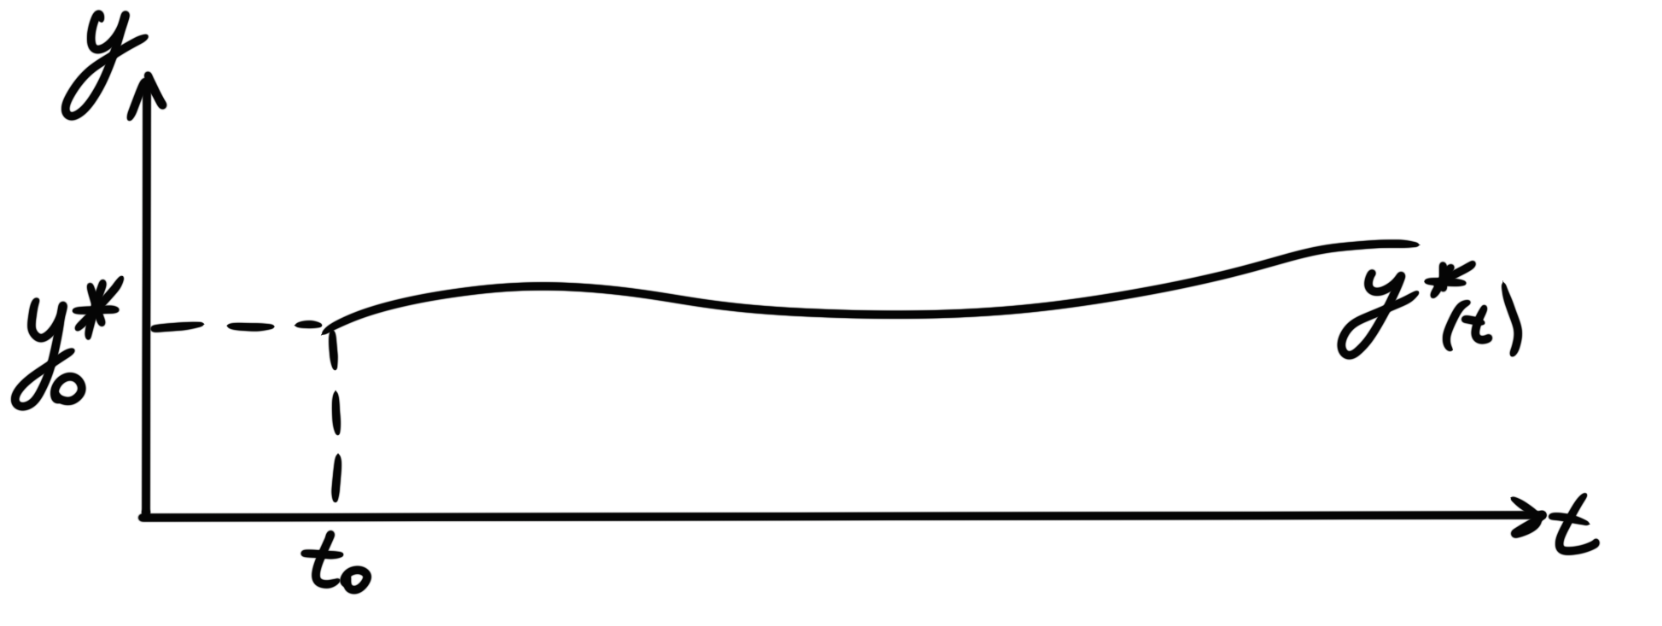
\includegraphics[width=0.6\textwidth]{/Users/vladbelousov/Desktop/Semestr_4-FP-NSU/ДфУ/Лекции_по_дням/image/31.png}
    \end{center}

    2) \( \exists \Delta > 0 \text{ }  \forall  \vec{y} _0 :   \left\lVert \vec{y } _ 0 - \vec{y } _0 ^*  \right\rVert< \Delta \Rightarrow \vec{y } (t )  \) тоже определенно от \( t_0  \) до \( +\infty  \)!

    \begin{center}
        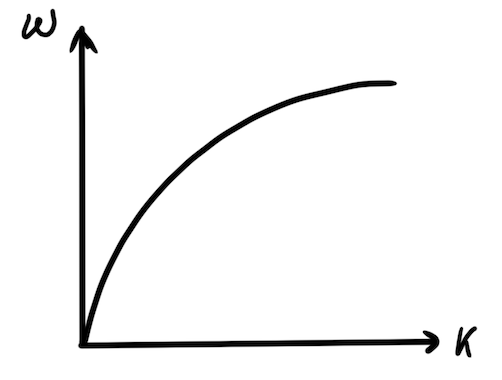
\includegraphics[width=0.6\textwidth]{/Users/vladbelousov/Desktop/Semestr_4-FP-NSU/ДфУ/Лекции_по_дням/image/32.png}
    \end{center}

    3) \( \forall  \varepsilon > 0 \text{ }  \exists  \delta > 0 \text{ }  \forall  \vec{y } _ 0 : \left\lVert  \vec{y } _0 - \vec{y }  ^ * _0  \right\rVert < \delta \Rightarrow \left\lVert  \vec{y }  (t ) - \vec{y }  ^*    (t ) \right\rVert < \varepsilon \text{ }  \forall  t \ge t_0 \) 

    \begin{center}
        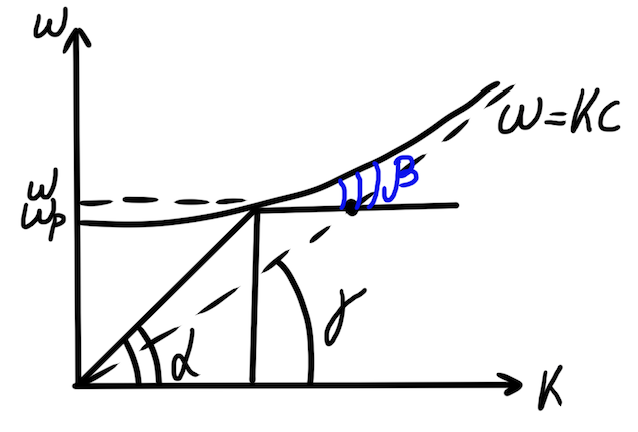
\includegraphics[width=0.6\textwidth]{/Users/vladbelousov/Desktop/Semestr_4-FP-NSU/ДфУ/Лекции_по_дням/image/33.png}
    \end{center}
\end{definition}

№1: Является ли устойчивое по Ляпунову решение задачи Коши: 

\[ \begin{cases}
y ' = 1 \\ 
y(0) = 0
\end{cases} \] 
\[ t_0 = 0, \text{ }  y^{* }  _0 = 0 , \text{ }  y^* (t )  = t \] 

1) \( y^* (t ) =t   \) определено от \( 0 \)  до \( + \infty  \)  (+)

\begin{center}
    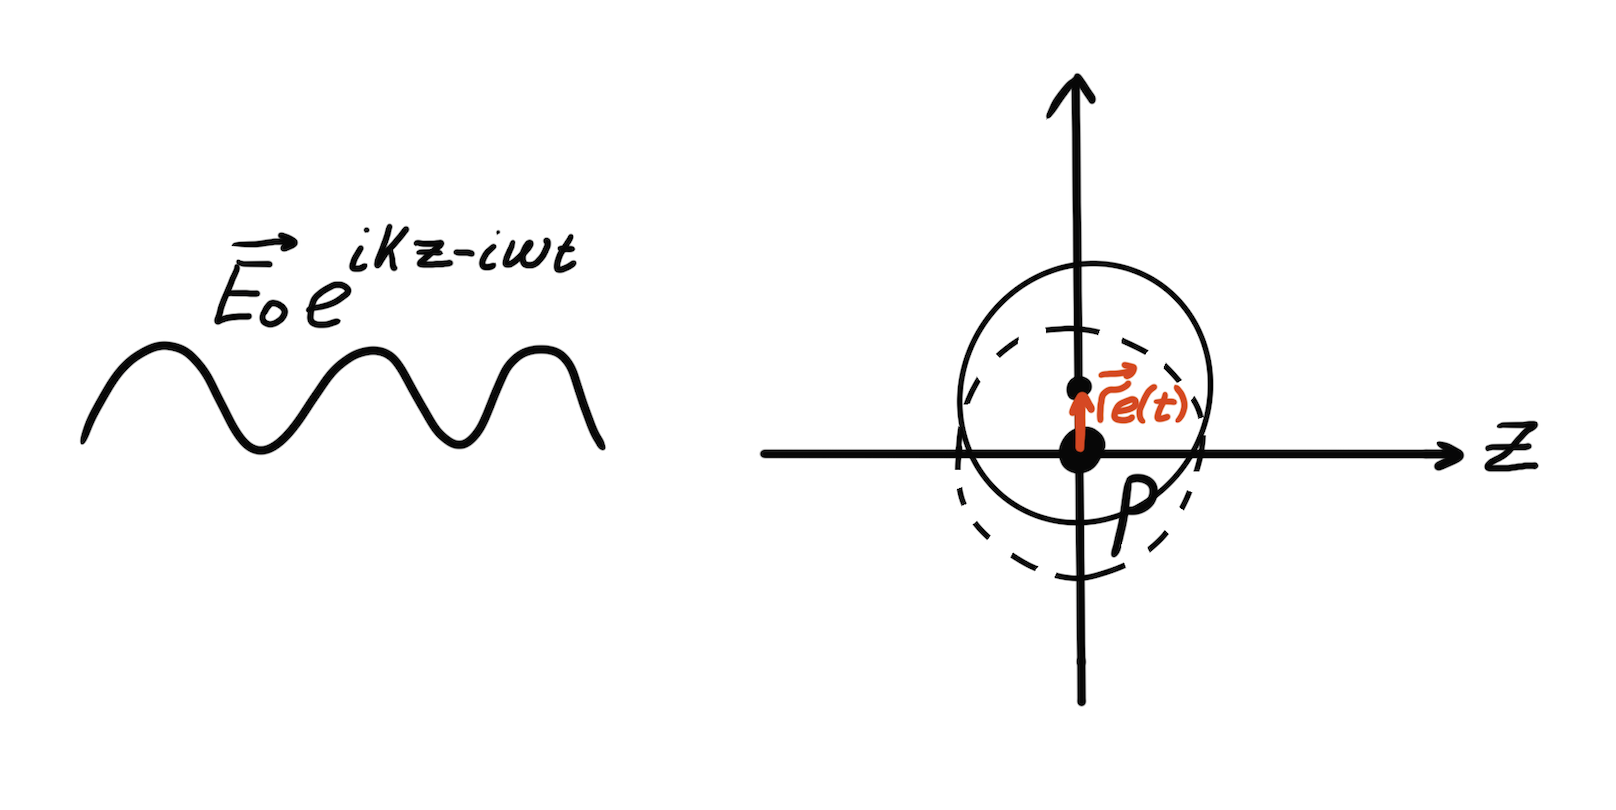
\includegraphics[width=0.4\textwidth]{/Users/vladbelousov/Desktop/Semestr_4-FP-NSU/ДфУ/Лекции_по_дням/image/34.png}
\end{center}

2) \( \begin{aligned}
    \begin{cases}
        y' = 1 \\ 
        y(0 )= 0 
    \end{cases}
    \Rightarrow y(t ) = t+ y_0
\end{aligned} \) (+)

\begin{center}
    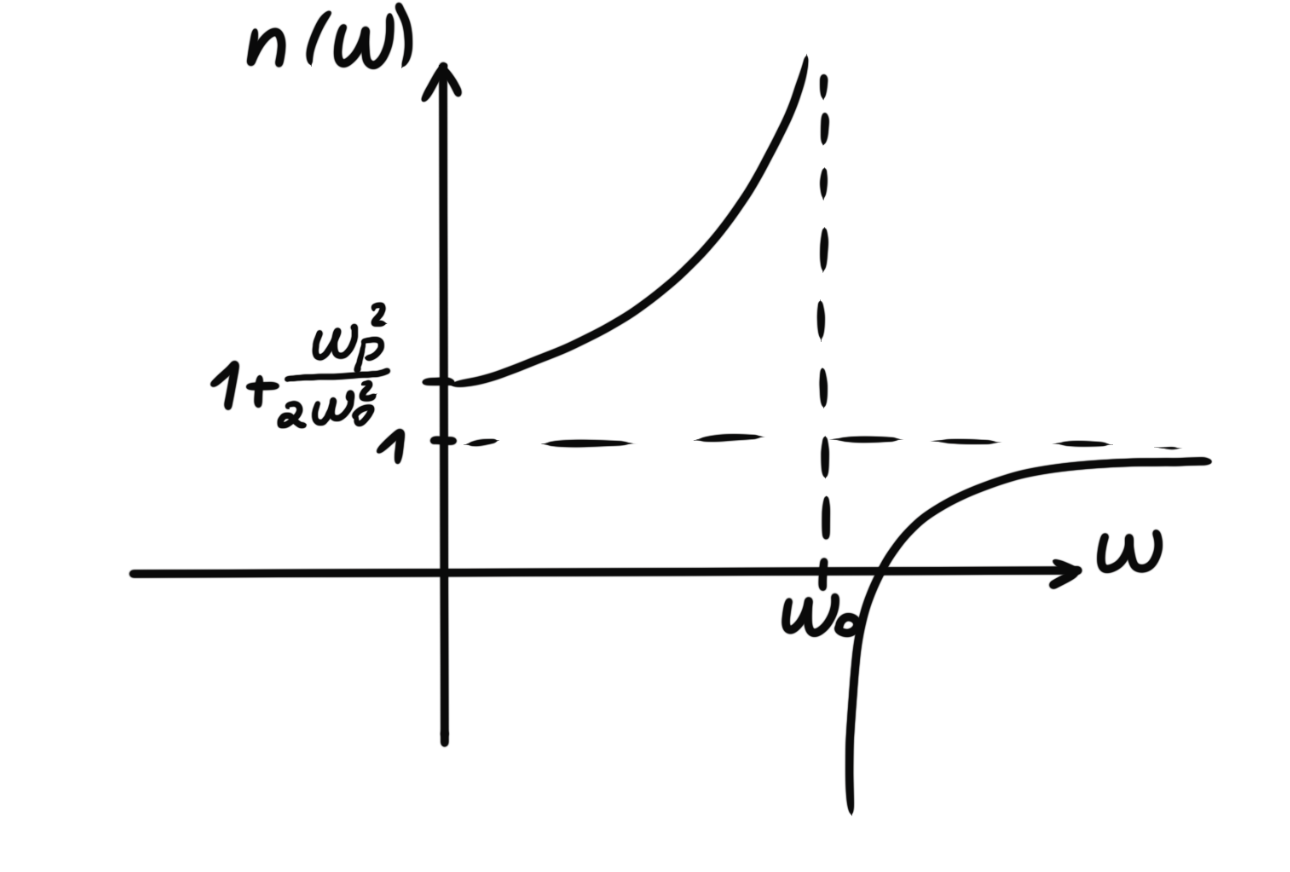
\includegraphics[width=0.4\textwidth]{/Users/vladbelousov/Desktop/Semestr_4-FP-NSU/ДфУ/Лекции_по_дням/image/35.png}
\end{center}

3) Надо показать: 

\[ \forall  \varepsilon > 0 \text{ }  \exists  \delta > 0 : \forall  y_0 : \left\lvert y_0  \right\rvert < \delta \Rightarrow\underbrace{ \left\lvert  y(t) - y^* (t )  \right\rvert}_{|y_0|} < \varepsilon \text{ } \forall  t \ge 0 \] 
\[ \delta = \varepsilon \Rightarrow \left\lvert y(t ) - y^ * (t )  \right\rvert = \left\lvert y_0 \right\rvert \] 

\begin{center}
    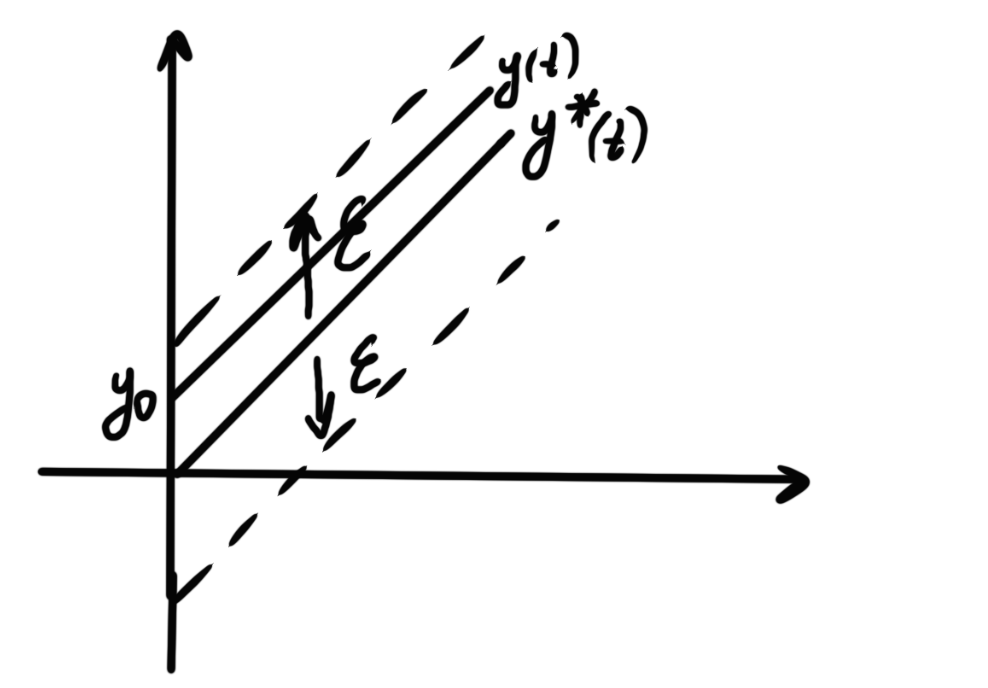
\includegraphics[width=0.4\textwidth]{/Users/vladbelousov/Desktop/Semestr_4-FP-NSU/ДфУ/Лекции_по_дням/image/36.png}
\end{center}

Ответ: \( y^* (t ) = t  \)  устойчиво по Ляпунову

\begin{definition}
    Решение \( \vec{y } ^* (t )  \) называется асимптотическим устойчивым, если: 

    1) \( \vec{y } ^* (t )  \) устойчиво по Ляпунову 

    2) \( \exists  \rho > 0 \text{ }  \forall  \vec{y } _0 : \left\lVert \vec{y } _ 0 - \vec{y }  ^* _0  \right\rVert < \rho \displaystyle \Rightarrow \lim_{t     \to \infty} \left\lVert \vec{y } (t ) - \vec{y}  ^* (t ) \right\rVert = 0  \) 

    \begin{center}
        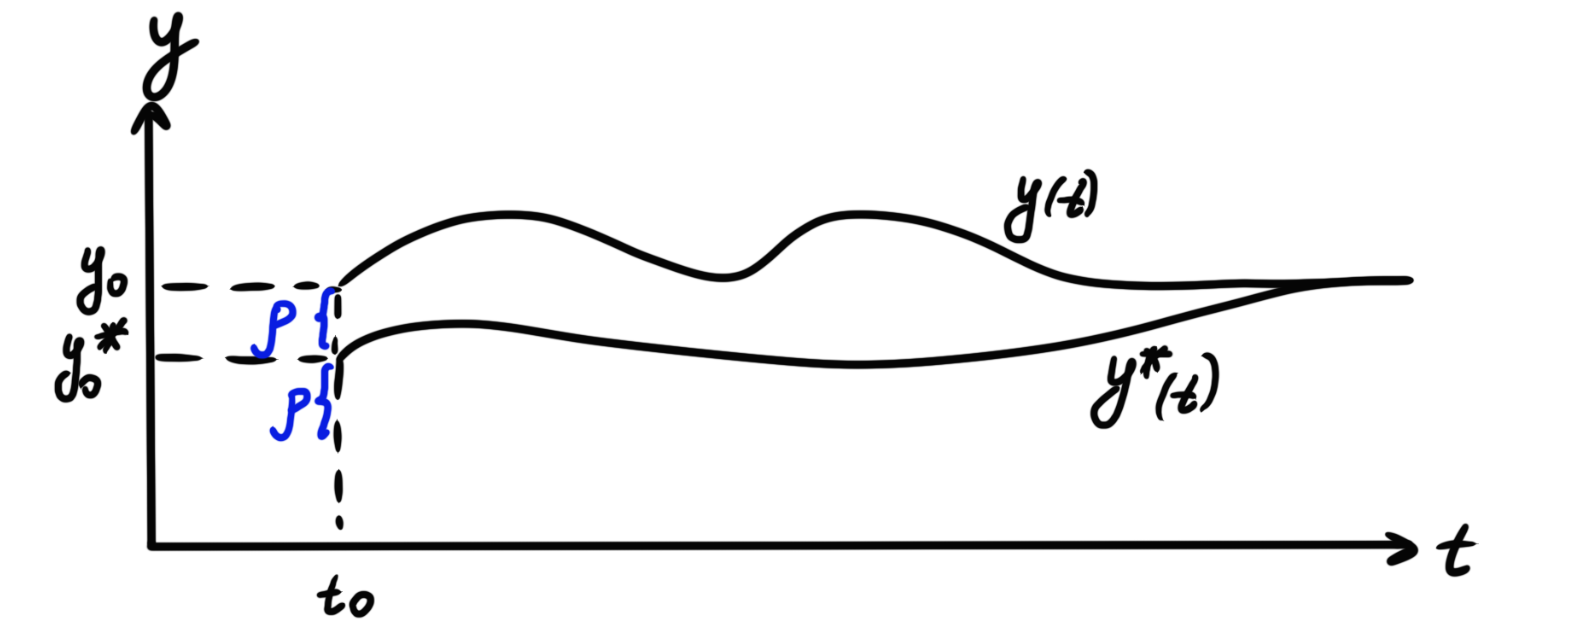
\includegraphics[width=0.6\textwidth]{/Users/vladbelousov/Desktop/Semestr_4-FP-NSU/ДфУ/Лекции_по_дням/image/37.png}
    \end{center}
\end{definition}

№2: Является ли устойчивое по Ляпунову асимптотическим устойчивым решение задачи Коши: 

\[ \begin{cases}
y ' = - y \\ 
y(0 )=  0
\end{cases} \] 
\[ t_0 = 0 , \text{ }  y_0 ^{* }  = 0  , \text{ }  y^{* }  (t ) = 0 \] 

\begin{center}
    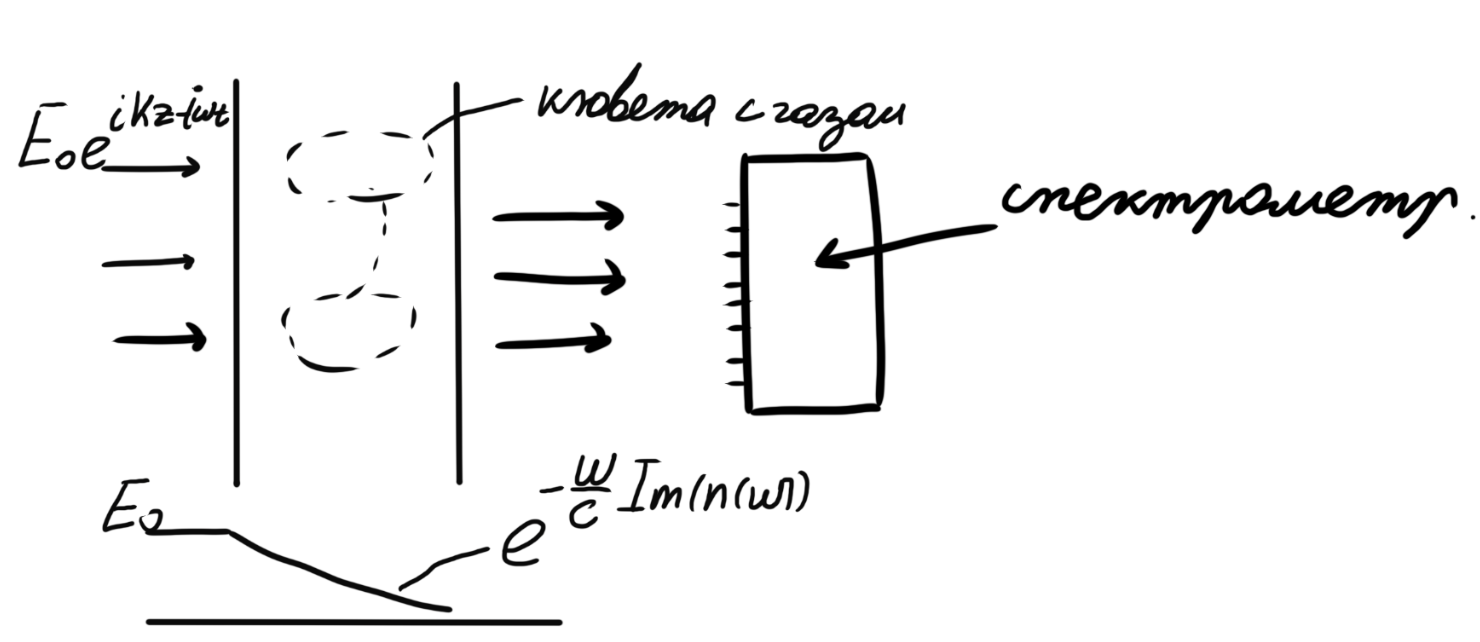
\includegraphics[width=0.4\textwidth]{/Users/vladbelousov/Desktop/Semestr_4-FP-NSU/ДфУ/Лекции_по_дням/image/38.png}
\end{center}

1) \( y^{* } (t ) = 0  \) определено на от \(  0 \)  до \( + \infty  \) (+)

2) \( \begin{aligned}
    \begin{cases}
        y ' = - y \\ 
        y(0 ) = y_0
    \end{cases}
    \Rightarrow y(t ) = e^{ - t } y_0 \text{ - определено на от } 0 \text{ до  }  + \infty  
\end{aligned} \) 

\begin{center}
    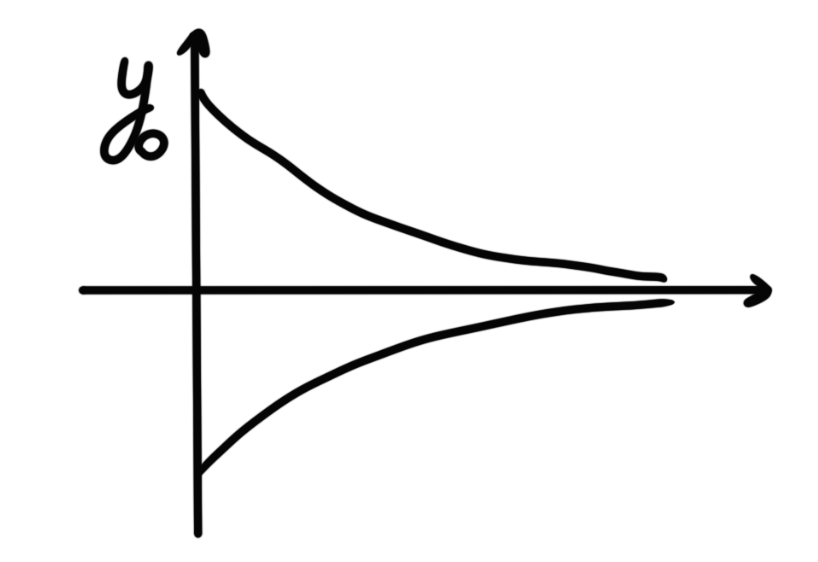
\includegraphics[width=0.4\textwidth]{/Users/vladbelousov/Desktop/Semestr_4-FP-NSU/ДфУ/Лекции_по_дням/image/39.png}
\end{center}

3) \( \forall  \varepsilon > 0 \text{ }  \exists  \delta > 0 \text{ }  \forall  y_0 : \left\lvert y_0  \right\rvert< \delta \Rightarrow \underbrace{\left\lvert y (t) \right\rvert}_{\left\lvert y_0 e^{ - t}  \right\rvert} < \varepsilon \text{ }  \forall  t \ge t_0 \) 

Возьмем \( \delta = \varepsilon  \) 

Если \( \left\lvert y_0      \right\rvert < \delta = \varepsilon \Rightarrow \left\lvert y(t ) \right\rvert = \left\lvert y_0 e^{ - t }  \right\rvert = \left\lvert y_0  \right\rvert e^{ -t } < \varepsilon  \Rightarrow \) нулевое решение \( y^* (t )   = 0\) устойчиво по Ляпунову

4) \( \displaystyle  \lim_{t  \to \infty} \left\lvert y(t) - y^* (t )  \right\rvert = \lim_{t  \to \infty}  \left\lvert y_0 e^{- t }  \right\rvert = 0\) 

\( \rho \) - любое \( \Rightarrow y^* (t ) =0\)   асимптотическим устойчиво. 

\begin{definition}
    Решение \( \vec{y } ^* (t )  \) называется неустойчивым, если оно не является устойчивым по Ляпунову, то есть если не выполняется хотя бы один пункт в определении устойчивости по Ляпунову.
\end{definition}

Не выполняется пункт 1: \( y^* (t ) \) не определено от \( 0 \) до \( + \infty  \) 

Не выполняется пункт 2: 

\( \forall  \Delta > 0 \text{ }  \exists  \vec{y } _0 : \left\lVert \vec{y}  _0 - \vec{y } ^* _0  \right\rVert < \Delta  \), \( \vec{y } (t ) \) не определено от \( t_0 \) до \( + \infty  \) 

Не выполняется пункт 3: 

\( \exists \varepsilon > 0 \text{ }  \forall  \delta > 0 \text{ }  \exists  \vec{y } _0 : \left\lVert  \vec{y }  _0 - \vec{y } _ 0 ^*  \right\rVert < \delta \Rightarrow   \exists  \hat{t }  \ge t_0 : \left\lVert \vec{y } (\hat{ t } )- \vec{y } ^*    (\hat{ t } )  \right\rVert \ge \varepsilon  \) 

№3: 

\[\begin{aligned}
    \begin{cases}
        y ' = 1 + y ^2 \\ 
        y(0 ) = 0
    \end{cases} 
    \Rightarrow y^* (t ) = \mathrm{tg }  (t ) 
\end{aligned}\] 

\begin{center}
    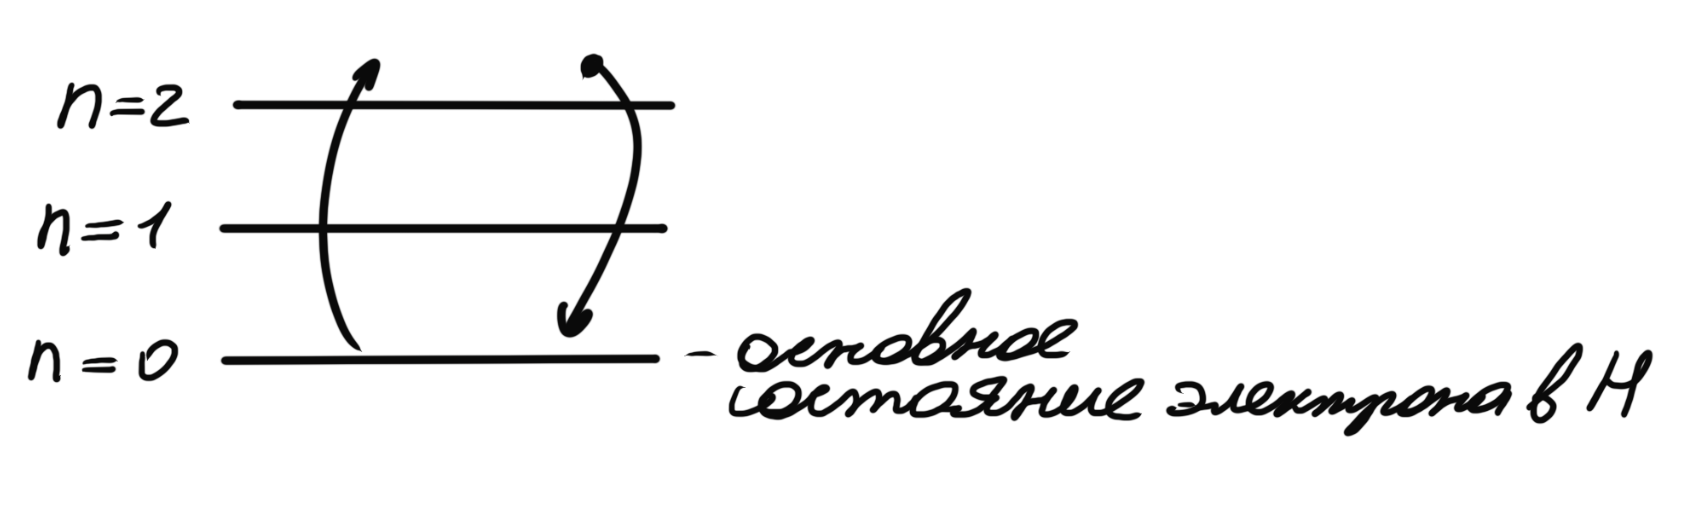
\includegraphics[width=0.3\textwidth]{/Users/vladbelousov/Desktop/Semestr_4-FP-NSU/ДфУ/Лекции_по_дням/image/40.png}
\end{center}

Не выполняется первый пункт \( \Rightarrow y^*(t ) = \mathrm{tg } (t ) \)  - неустойчиво. 

№4: 

\[ \begin{aligned}
    \begin{cases}
        y ' = y ^2 \\ 
        y(0 ) = 0
    \end{cases}
    \Rightarrow y^* (t ) = 0
\end{aligned} \] 

\begin{center}
    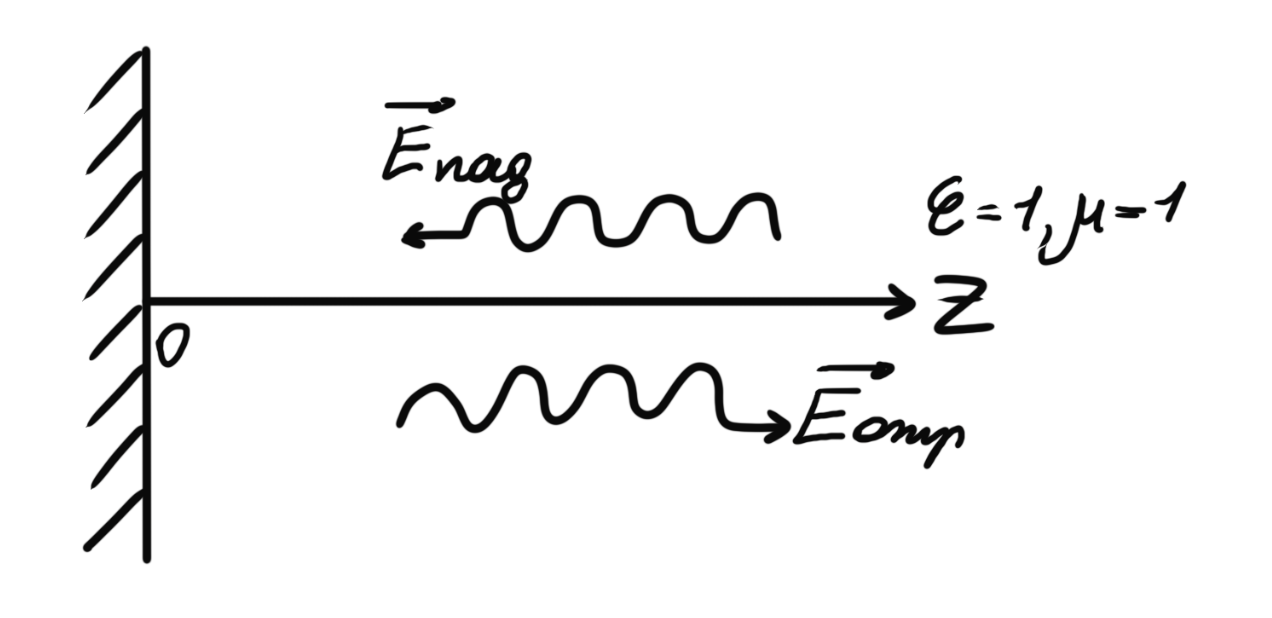
\includegraphics[width=0.4\textwidth]{/Users/vladbelousov/Desktop/Semestr_4-FP-NSU/ДфУ/Лекции_по_дням/image/41.png}
\end{center}

1) (+) \\



2) \( \begin{aligned}
\begin{cases}
    y' = y ^2 \\ 
    y(0 ) = y_0
\end{cases}
\Rightarrow y(t ) = \frac{1}{\displaystyle  \frac{1}{y_0 } -t  } 
\end{aligned} \) 

\[ y(t ) \text{ при }  y_0> 0 \text{ не определено от } 0 \text{ до }  + \infty   \Rightarrow 2) \text{ не выполняется}\Rightarrow y^{* } (t )= 0 \text{ - неустойчиво}  \] 

№5: 

\[ \begin{aligned}
\begin{cases}
y ' = y \\ 
y(0 ) = 0 
\end{cases}
\Rightarrow y^* (t ) = 0
\end{aligned} \] 

1) \( y^*  (t ) = 0\)  определено от \( 0 \) до \( + \infty  \)  (+)

2) \[ \begin{aligned}
\begin{cases}
y ' = y \\ 
y(0 ) = y_0 
\end{cases}
\Rightarrow y(t ) = y_0 e^{t } 
\end{aligned} \]

\begin{center}
    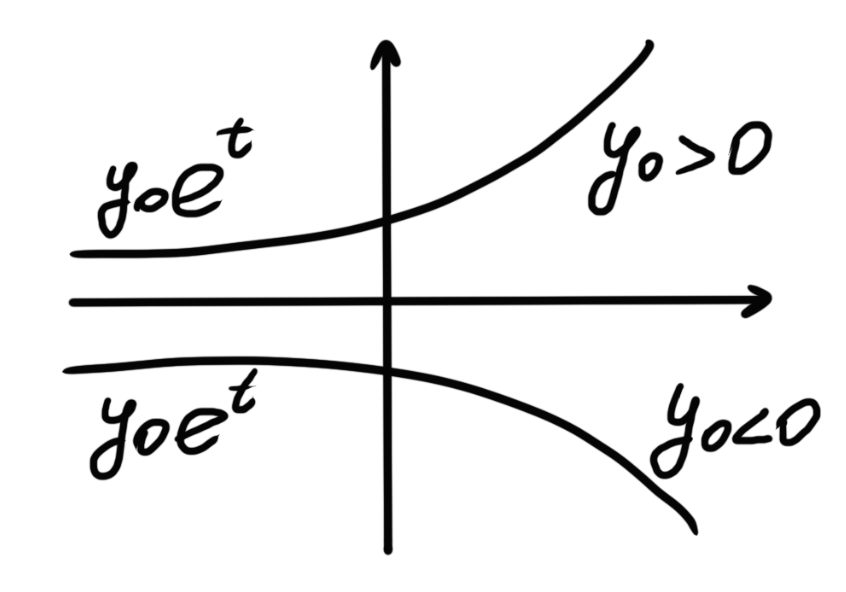
\includegraphics[width=0.4\textwidth]{/Users/vladbelousov/Desktop/Semestr_4-FP-NSU/ДфУ/Лекции_по_дням/image/42.png}
\end{center}

\[ y(t) \text{ определено от } 0 \text{ до }  + \infty  \quad  (+)  \] 

3) 

\begin{center}
    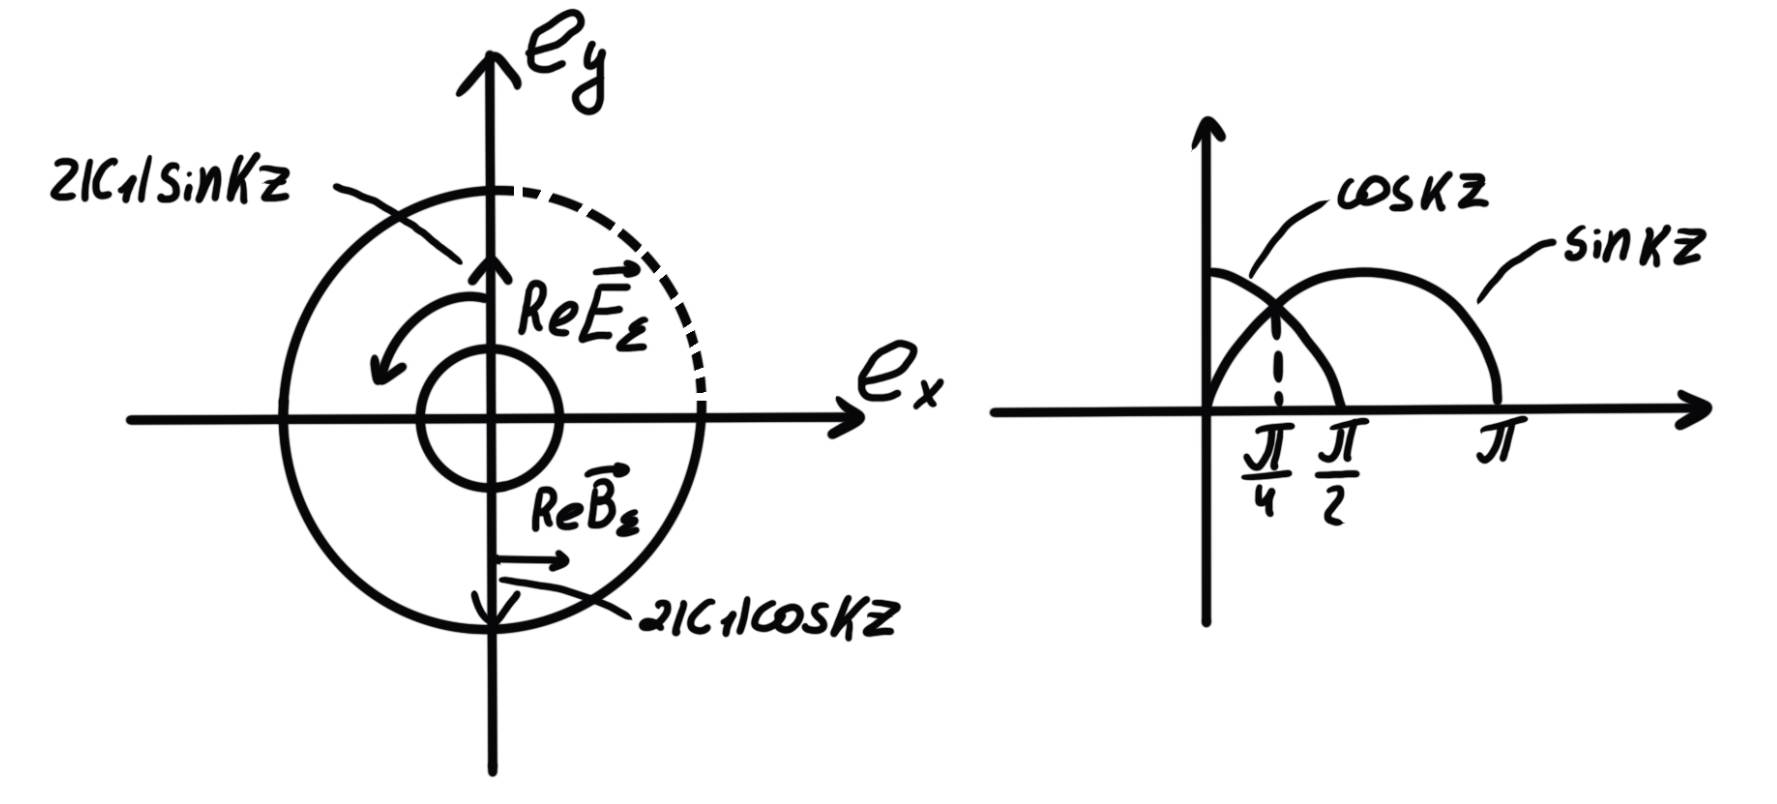
\includegraphics[width=0.4\textwidth]{/Users/vladbelousov/Desktop/Semestr_4-FP-NSU/ДфУ/Лекции_по_дням/image/43.png}
\end{center}

\[ \exists  \varepsilon = 10 \text{ }  \forall  \delta > 0 : \exists  y_0= \frac{\delta}{2 } : \left\lvert y_0  \right\rvert < \delta  \] 
\[ \exists \hat{ t }  : \left\lvert y(\hat{t }  ) \right\rvert \ge \varepsilon = 10 \] 
\[ \left\lvert y_0 e^{\hat{t } }  \right\rvert = \frac{\delta}{2 } e^{\hat{ t } } \] 

\[ \frac{\delta}{2 }  e^{\hat{ t } } \ge 10 \Rightarrow \hat{ t }  = \ln \left( \frac{20}{\delta}  \right)  \] 

Нулевое решение \( y^* (t ) = 0\)  неустойчиво.
%%-------------------------------%%

% Закрытие документа, если файл компилируется отдельно
\ifdefined\mainfile
    % Если это основной файл, не нужно заканчивать документ
\else
    \end{document}
\fi
% Условная компиляция для самостоятельной работы
\ifdefined\mainfile
    % Если это часть основного файла, не добавляем начало и конец документа
\else
    \documentclass[12pt, a4paper]{report}
    \usepackage{/Users/vladbelousov/Desktop/Semestr_4-FP-NSU/Настройка/library}
    \usepackage[utf8]{inputenc} % Подключение поддержки UTF-8
    \begin{document}
\fi

%%-------------------------------%%

\section{Сведение задачи  об устойчивости  произвольного решения к задаче об устойчивости нулевого решения}

\[ \frac{d}{dt }  \vec{y} = \vec{f } (t, \vec{y} ) \tag{1}  \] 
\( \vec{y} ^{* } (t) \)  - решение, которое мы хотим исследовать на устойчивость. 

Предположим, что \( \vec{y } ^* (t) \) определенно от \( t_0 \) до \( +\infty  \).

Пусть \( \vec{y} (t) \)  - другое решение системы (1). Замена \( \vec{z }(t )= \vec{y } (t) - \vec{y }^{* } (t)   \) 

\[ \frac{d}{dt }  \vec{z } (t ) = \frac{d}{dt }  \vec{y} (t )- \frac{d}{dt }  \vec{y } ^*   (t ) = \vec{f } (t, \vec{y} (t))-\vec{f } (t, \vec{y } ^{* } (t)) =  \vec{f } (t, \vec{y}^* (t) +\vec{z } (t))-\vec{f } (t, \vec{y } ^{* } (t))\] 
\[ \frac{d}{dt }\vec{z } (t) =   \vec{f } (t, \vec{y}^* (t) +\vec{z } (t))-\vec{f } (t, \vec{y } ^{* } (t)) \tag{2} \] 

\( \vec{z } ^{* } (t) = 0\)  - решение системы (2). 

\begin{theorem}
    Решение \( \vec{y } ^{* } (t) \)  системы (1) устойчиво по Ляпунову/асимптотически устойчиво/неустойчиво \( \Leftrightarrow  \) нулевое решение \( \vec{z } ^{* } (t) = 0 \) системы (2) устойчиво по Ляпунову/асимптотически устойчиво/неустойчиво. 
\end{theorem}

\begin{proof} \(  \) 

По определению \( \vec{z } ^*   (t ) = 0 \) устойчиво по Ляпунову, если: 

1) \( \vec{z } ^* (t) = 0 \) определено от \( t_0 \) до \( +\infty  \) 

2) \( \exists  \Delta > 0 \text{ }  \forall  \vec{z } (t_0): \left\lVert  \vec{z } (t_0 )- \vec{z } ^* (t_0 ) \right\rVert < \Delta \Rightarrow \vec{z } (t) \) тоже определено от \( t_0 \) до \( \infty  \), где \( \vec{z} ^{* } (t_0 )= 0  \), а \( \vec{z } (t_0 )  = \vec{y } (t_0 )- \vec{y } ^* (t_0) \).

3) \( \forall  \varepsilon > 0 \text{ } \exists  \delta > 0  \text{ }  \forall  \vec{z } (t_0) : \left\lVert \vec{z } (t_0 ) - \vec{z } ^* (t_0 ) \right\rVert < \delta \Rightarrow \left\lVert \vec{z } (t ) - \vec{z } ^* (t) \right\rVert < \varepsilon \text{ }  \forall  t \ge  t_0 \), где   \( \vec{z} ^{* } (t_0 )= 0  \), а \( \vec{z } (t_0 )  = \vec{y } (t_0 )- \vec{y } ^* (t_0) \) и  где \( \vec{z} ^{* } (t )= 0  \), а \( \vec{z } (t)  = \vec{y } (t )- \vec{y } ^* (t) \)

\end{proof}

\[ \frac{d}{dt }  \vec{y } (t ) = A (t ) \vec{y } + \vec{ g } (t) = \vec{f } (t,\vec{y } )   \tag{3}  \] 
, где \( \displaystyle A(t ) = (a_{ij }(t) ) , \text{ }  \vec{g } (t ) = \begin{pmatrix}
g_1\\
\vdots\\
g_n
\end{pmatrix} , \text{ }  a_{ij }  (t ) , g_j(t )\in  C(\mathbb{R}) \) 

Так как система линейна, то любое решение определенно на \( \mathbb{R} \). 

\( \Rightarrow  \) пункты 1) и 2) в определении устойчивости выполнены автоматически. 

Замена \( \vec{z } (t) = \vec{y } (t )- \vec{y }^* (t)\), где  \( \vec{y } (t) \)   - другое решение (3). 

\[ \frac{d}{dt }  \vec{z }  = \vec{f } (t, \vec{y } ^* +\vec{z } ) - \vec{f } (t, \vec{y } ^*)  = A(t )\vec{z} \tag{4}\] 
, где \( \vec{z }^* (t )= 0 \)  - решение (4). 

\begin{theorem}
    Решение \( \vec{y } ^{* } (t) \) линейной неоднородной  системы (3) устойчиво по Ляпунову/асимптотически устойчиво/неустойчиво \( \Leftrightarrow  \) нулевое решение \( \vec{z } ^{* } (t) = 0 \) линейной неоднородной системы (4) устойчиво по Ляпунову/асимптотически устойчиво/неустойчиво. 
\end{theorem}

\textbf{Следствие 1.} На устойчивость решения линейной неоднородной системы (3) не влияет \( \vec{g } (t) \), а влияет  только \( A(t). \) 

\textbf{Следствие 2.} Все решения линейной системы (3) либо одновременно устойчивы, либо одновременно неустойчивы. 

\section{Устойчивость линейных системах}

\[ \frac{d}{dt }  \vec{y }  = A (t ) \vec{y } \tag{1}  \] 
, где \( \displaystyle  A (t ) = (a_{ij } (t)) , \text{ }  a_{ij }(t) \in  C(\mathbb{R})  \) 

\( \vec{y } ^* (t ) = 0 \) -  решение, которое мы исследуем на устойчивость. 

\begin{theorem}
    Нулевое решение  \( \vec{y } ^{* }  (t )  = 0 \) системы (1) устойчиво по Ляпунову \( \Leftrightarrow  \) все решения системы (1) ограничены вправо, то есть \( \forall   \) решения \( \vec{y } (t) \text{ }  \exists  M >0 \)  \( \left\lVert \vec{y} (t) \right\rVert \le M \text{  } \forall t \ge  t_0 \) 
\end{theorem}

\begin{proof} \(  \) 

    \( (\Rightarrow):\) 

    По определению: \( \forall  \varepsilon > 0 \text{ }  \exists  \delta > 0 \text{ }  \forall  \vec{y } _0 < \delta \Rightarrow \left\lVert \vec{y } (t) \right\rVert < \varepsilon \text{ }  \forall  t \ge  t_0 \) 


    Пусть \( \vec{y} (t ) \neq 0 \) - решение системы (1). Возьмем  \( \vec{v } (t ) =\displaystyle  \underbrace{\frac{\delta}{2 \left\lVert \vec{y } (t_0) \right\rVert }}_{\mathrm{const}   } \vec{y } ( t)  \) - тоже решение.

    \[ \left\lVert \vec{v} (t_0 ) \right\rVert  = \left\lVert \frac{ \delta }{2 \left\lVert \vec{y } (t_0 ) \right\rVert } \vec{y  } (t)  \right\rVert = \frac{ \delta }{2 \left\lVert \vec{y } (t_0) \right\rVert} \left\lVert \vec{y } (t_0) \right\rVert = \frac{\delta}{2 }  < \delta  \] 

    Из определения: \( \forall  \varepsilon > 0 \text{ } \exists  \delta > 0 \text{ }  \forall  \vec{v } (t ) : \left\lVert \vec{v }  (t_0) \right\rVert < \delta \Rightarrow \left\lVert \vec{v }  (t ) \right\rVert < \varepsilon \text{ }  \forall  t \ge  t_0 \) 

    \[ \left\lVert \frac{\delta }{2 \left\lVert  \vec{y } (t_0) \right\rVert } \vec{y } (t)  \right\rVert < \varepsilon \Rightarrow \left\lVert \vec{y } (t) \right\rVert < \varepsilon \frac{ 2 \left\lVert \vec{y } (t_0) \right\rVert}{\delta } = M  \] 

    \( (\Leftarrow): \) 

    Пусть \( \forall  \) решения \( \vec{y} (t ) \text{ } \exists  M > 0 : \left\lVert \vec{y } (t) \right\rVert \le  M \text{  } \forall  t \ge  t_0 \)  

    Все решения системы (1): \( \vec{y } (t ) = F(t ) \vec{c} = c_1 \vec{\varphi}_1 (t ) +... + c_n \vec{\varphi }_n(t)   \). 

    Возьмем \( F (t) \) - ФМР (фундаментальная матрица решений) такую, что \( F(t_0 ) = E\) 

    \[ \begin{aligned}
        \begin{cases}
            \displaystyle \frac{d}{dt }  \vec{ y } =   A(t )\vec{y } \\[5pt]
            \vec{y }  (t_0 )= \vec{y } _0
        \end{cases} 
        \Rightarrow \vec{y } (t ) = F(t ) \vec{c}= F(t ) \vec{y } _0 = y_{01} \vec{\varphi }_1 (t ) +...+ y_{0n }  \vec{\varphi }_n (t )   
    \end{aligned}\] 
    , где \( \displaystyle  \vec{y}_0 = \begin{pmatrix}
    y_{01}  \\
    \vdots\\
    y_{0n} 
    \end{pmatrix}, \text{ }  F(t ) = (\vec{\varphi }_1 (t ) |...|\vec{\varphi }_n(t)  )  \) 

    Так как \( \vec{\varphi }_1 (t ),..., \vec{\varphi }_n (t)   \) - решения, то \( \exists  M_1, \ldots, M_n : \left\lVert \vec{\varphi}_1  (t ) \right\rVert \le  M_1 ,..., \left\lVert  \vec{\varphi }_n (t) \right\rVert \le M_n \text{ }  \forall  r \ge  t_0 \) 

    Для решения задачи Коши: 

    \[ \left\lVert \vec{y } (t) \right\rVert  = \left\lVert y_{01} \vec{\varphi }_1 (t ) +...+ y_{0n } \vec{\varphi }_n(t)   \right\rVert \le \left\lvert y_{01} \right\rvert \left\lVert \vec{\varphi}_1 (t )  \right\rVert +...+ \left\lvert y_{0n }  \right\rvert \left\lVert  \vec{\varphi} _n (t) \right\rVert \le  \left\lvert y_{01} \right\rvert M_1+ ... + \left\lvert y_{0n}   \right\rvert M_n \le  \] 
    \[ \le  \underbrace{\max  \{M_1, \ldots, M_n\}}_{= \tilde{M}} (\left\lvert y_{01} \right\rvert + ...+ \left\lvert  y_{0n}  \right\rvert) = \tilde{M } \left\lVert \vec{y } _0 \right\rVert _1 \] 

    Возьмем норму \( \left\lVert \vec{y } _0 \right\rVert _1 = (\left\lvert y_{01} \right\rvert + ...+ \left\lvert y_{0n}  \right\rvert) \) 

    Если \( \left\lVert  \vec{y } _0  \right\rVert _ 1 < \delta \Rightarrow \left\lVert \vec{y } (t) \right\rVert  \le  \tilde{M } \left\lVert \vec{y} _0 \right\rVert _1  < \tilde{M }\delta \overset{(*)}{= }\varepsilon \), \( (*): \)  возьмем \( \delta =\displaystyle  \frac{\varepsilon}{\tilde{ M}}  \) 

    \( \Rightarrow  \vec{y } ^* (t) = 0\)  устойчиво по Ляпунову. 

\end{proof}

\begin{theorem}
    Нулевое решение \( \vec{y } ^{* } (t) = 0 \) системы (1) асимптотически устойчиво \( \Leftrightarrow  \) \( \forall  \) решения \( \vec{y } (t) \) выполняется \( \left\lVert \vec{y } (t) \right\rVert \xrightarrow{t \to  +\infty  } 0   \).
\end{theorem}

\begin{proof} \(  \) 

    \( (\Rightarrow): \) 

    Из определения асимптотической устойчивости: \( \exists  \rho> 0 \text{ }  \forall  \vec{y } _ 0 : \left\lVert \vec{y }  _0 \right\rVert < \rho \Leftrightarrow  \left\lVert \vec{y } (t) \right\rVert \xrightarrow{t \to  + \infty } 0   \) 

    Пусть \( \vec{y } (t)\neq 0  \)  - решение системы (1). Возьмем \( \vec{v } (t) =\displaystyle  \frac{ \rho }{2 \left\lVert \vec{y } (t_0) \right\rVert} \vec{y } (t)  \)  - тоже решение. 

    \[ \left\lVert \vec{v }  (t ) \right\rVert = \left\lVert \frac{\rho}{2 \left\lVert \vec{y } (t_0) \right\rVert} \vec{y } (t)   \right\rVert = \frac{\rho}{ 2 \left\lVert \vec{y } (t_0)  \right\rVert} \left\lVert \vec{y } (t_0) \right\rVert = \frac{\rho}{2 }  <\rho \] 

    \( \Rightarrow \) по определению асимптотической устойчивости: \( \displaystyle \lim_{t \to \infty } \left\lVert \vec{v} (t)  \right\rVert 0  \) 

    \[ \lim_{t  \to +\infty} \left\lVert \frac{\rho}{2 \left\lVert \vec{y } (t_0) \right\rVert } \vec{y} (t)  \right\rVert = 0 \Rightarrow \lim_{t \to +\infty}  \left\lVert \vec{y } (t) \right\rVert = 0 \] 

    \( (\Leftarrow): \) 

    Пусть \( \forall   \) решения \( \vec{y } (t) \)  выполняется \( \displaystyle \left\lVert \vec{y } (t) \right\rVert \xrightarrow{ t \to  + \infty } 0    \) 

    Хотим доказать:
    
    1) \( \vec{y } ^* (t)  \) устойчиво по Ляпунову. По Теореме 1. достаточно доказать, что все решения ограничены вправо. 

    По определению предела: \( \displaystyle  \left\lVert \vec{y } (t ) \right\rVert \xrightarrow{ t \to  +\infty } 0   \) 

    \[ \forall  \sigma > 0 \text{ }  \exists  T \text{ }  \forall  t \ge  T : \left\lVert \vec{y } (t) \right\rVert < \sigma \]  

    \( \vec{y } (t) \) - непрерывна, \( [t_0, T] \) - компакт \( \Rightarrow \left\lVert \vec{y } (t) \right\rVert \le  c \text{ }  \forall  t \in  [t_0 , T] \) 

    \( \Rightarrow \left\lVert  \vec{y } (t) \right\rVert \le  \max  \{\sigma, c \} , t \ge  t_0 \Rightarrow  \)  по Теореме 1. \( \vec{y } ^* (t ) = 0  \) устойчиво по Ляпунову. \\

    2) Надо проверить: \( \exists  \rho > 0 \text{ } \forall  \vec{y } _0 : \left\lVert \vec{y } _0  \right\rVert < \rho \Rightarrow \displaystyle \lim_{t \to +\infty} \left\lVert \vec{y } (t) \right\rVert = 0  \) 

    \begin{center}
        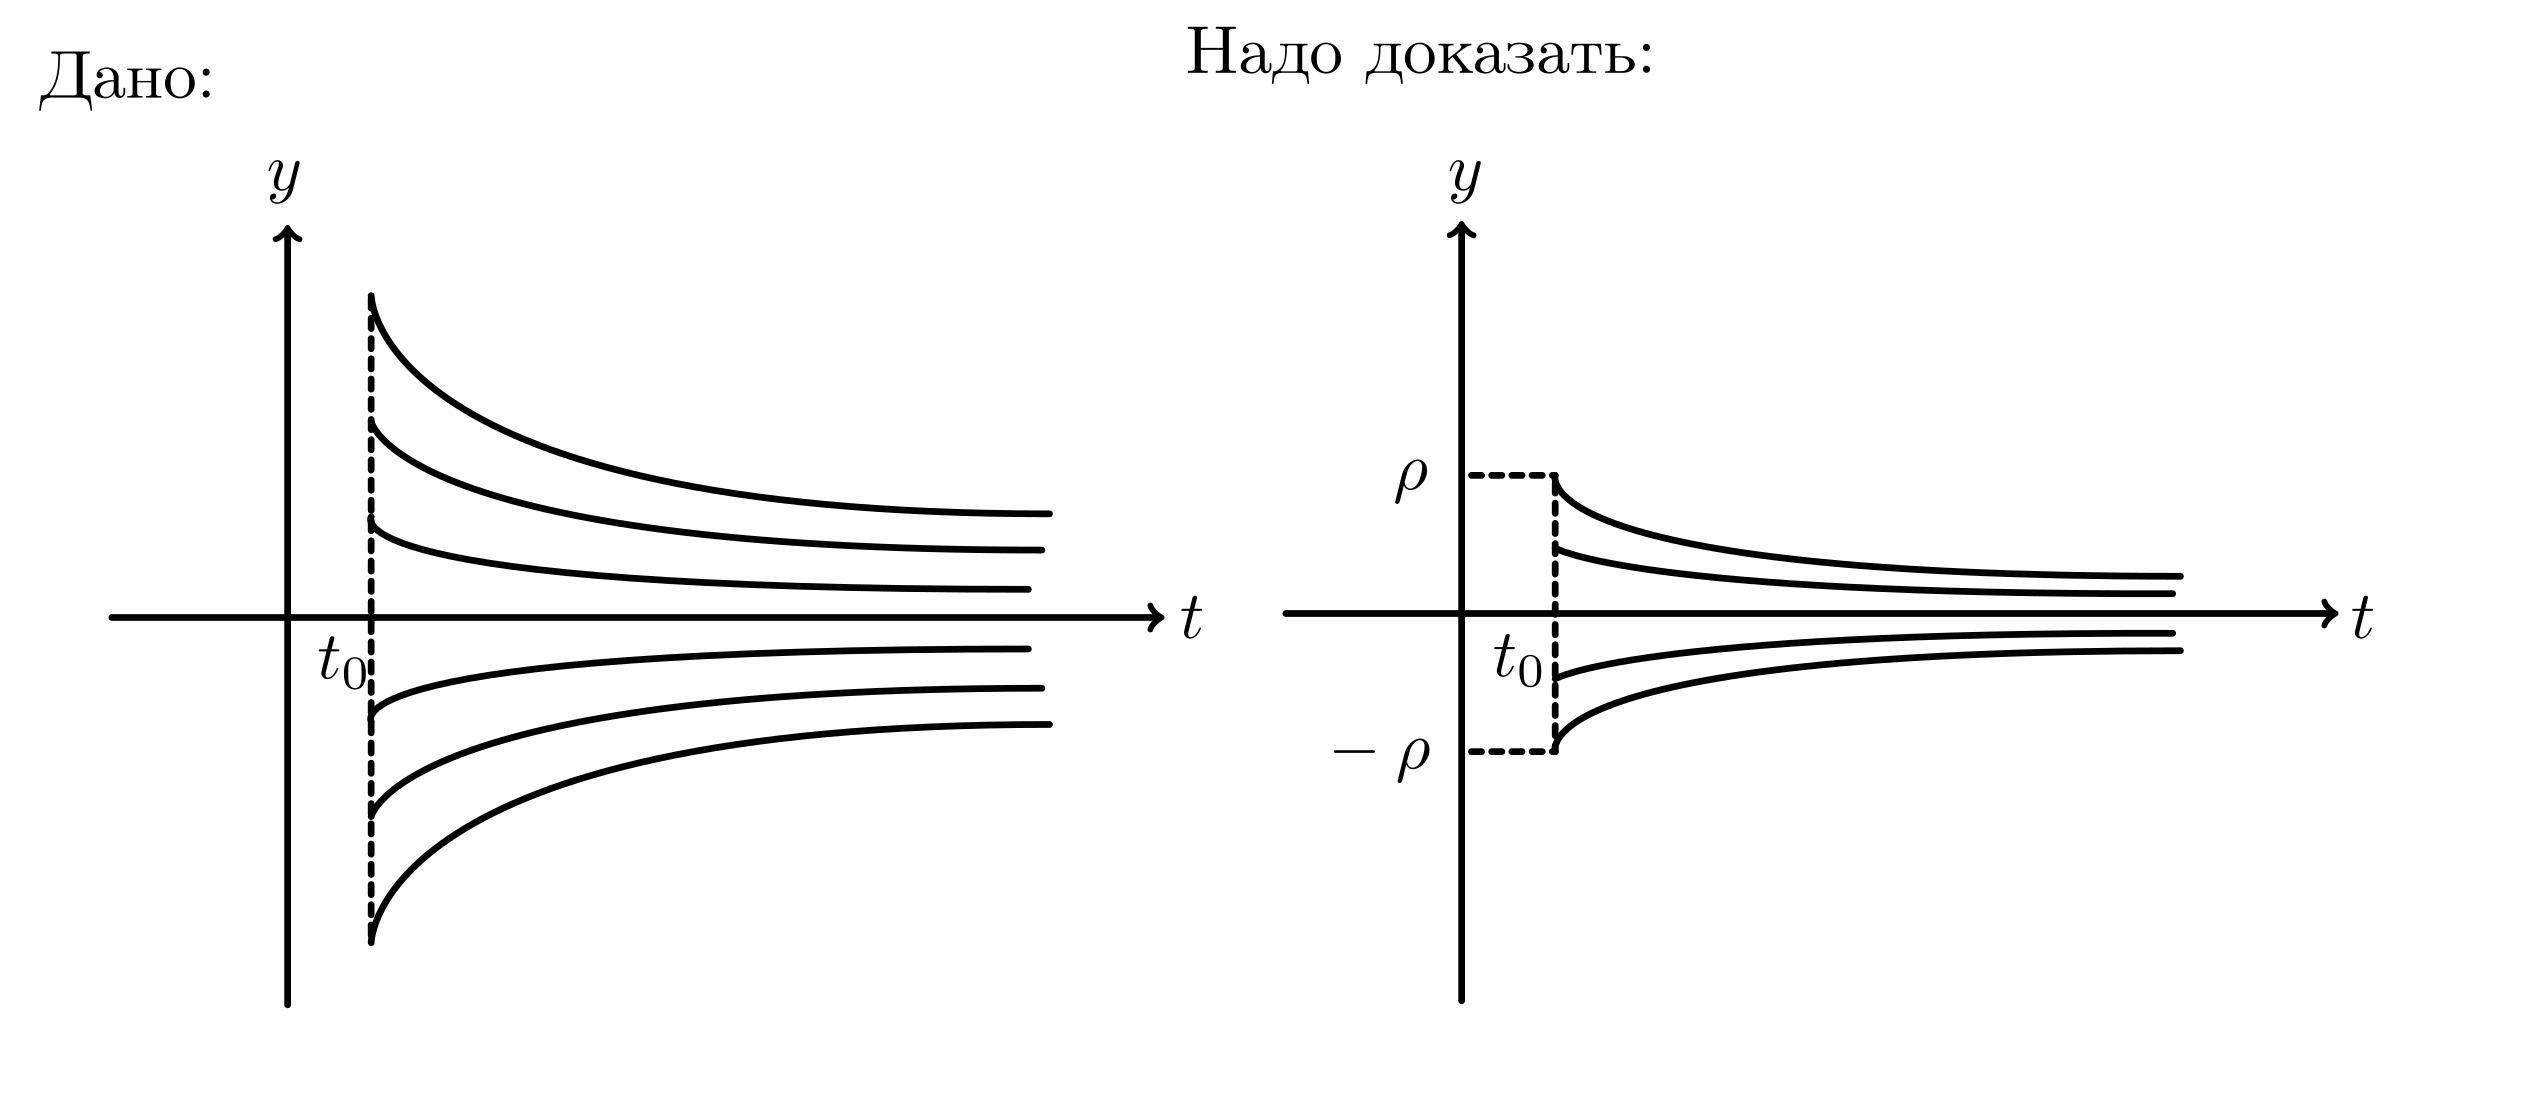
\includegraphics[width=0.84\textwidth]{/Users/vladbelousov/Desktop/Semestr_4-FP-NSU/ДфУ/Лекции_по_дням/image/44.png}
    \end{center}


    Возьмем \( \rho = 1 \), тогда 2) пункт выполняется. 

    \[ \vec{ y } ^{* } (t )  = 0  \text{ асимптотически устойчиво.} \] 

\end{proof}

\[ \frac{d}{dt }  \vec{y } = A y \tag{2} \] 
, где \( \displaystyle  A (t ) = (a_{ij } ) , \text{ }  a_{ij } \in  C(\mathbb{R})  \)

Все решения \( \vec{y } (t) = e^{ t A }  \vec{ c }  = T e^{ t Y }  \vec{b} \).



%%-------------------------------%%

% Закрытие документа, если файл компилируется отдельно
\ifdefined\mainfile
    % Если это основной файл, не нужно заканчивать документ
\else
    \end{document}
\fi
% Условная компиляция для самостоятельной работы
\ifdefined\mainfile
    % Если это часть основного файла, не добавляем начало и конец документа
\else
    \documentclass[12pt, a4paper]{report}
    \usepackage{/Users/vladbelousov/Desktop/Semestr_4-FP-NSU/Настройка/library}
    \usepackage[utf8]{inputenc} % Подключение поддержки UTF-8
    \begin{document}
\fi

%%-------------------------------%%
\[ \lambda_1, \ldots, \lambda_n \text{  - собственные числа матрицы } A  \] 

\begin{theorem}
    Нулевое решение \( \vec{y } ^* (t )= 0\) системы (2) асимптотически устойчиво \( \Leftrightarrow  \forall  \lambda_1, \ldots, \lambda_n :  \mathrm{Re } \lambda_j < 0 , \text{ }  j=1, \ldots, n \).
\end{theorem}

\begin{proof} \(  \) 

    \( (\Rightarrow): \)

    От противного. Пусть \( \exists  \lambda_k : \mathrm{Re } \lambda_k \ge  0  \). Взять решение \( \vec{y } (t ) =  e^{ \lambda_k t } \vec{v }_k , \text{ }  \vec{v } _k \) - собственный вектор, соответственного \( \lambda_k \). 

    \[ \left\lVert  \vec{y } (t) \right\rVert = \left\lVert e^{\lambda_k t } \vec{v } _k   \right\rVert = \left\lvert e^{ \lambda_k t }  \right\rvert \left\lVert  \vec{v }  _k  \right\rVert  = e^{\mathrm{Re } \lambda_k t  } \underbrace{\left\lVert \vec{v } _k  \right\rVert}_{\neq 0} \cancel{\xrightarrow{ t \to  +\infty }} 0    \] 
    \( \Rightarrow \) нулевое решение не асимптотически устойчиво. Противоречие \( \Rightarrow  \forall  \lambda_j \text{ }  \mathrm{Re }  \lambda_j < 0  \) 

    \( (\Leftarrow): \) 

    Пусть \( \forall  \lambda_j \text{ }  \mathrm{Re }  \lambda_j < 0   \). Все решения системы \( \vec{y } (t ) = c_1 \vec{\varphi }_1 (t )+ ... + c_n \vec{\varphi }_n (t)   \) 
    
    \[ \lambda_1 \to \underbrace{ \vec{v } _c , \vec{v } _{\text{ пр}_1 },...,  \vec{v } _{\text{ пр}_{m-1} }}_{m \text{ - векторов} }  \] 

    \[ \begin{aligned}
        \begin{cases}
            \vec{\varphi }_1 (t ) = e^{ \lambda_1 t } \vec{v } _{\text{ с} }  \\
            \vec{\varphi }_2  (t ) = e^{ \lambda_1t }(  \vec{v } _{\text{ с} }t +\vec{ v } _{\text{пр}_{1}}  )\\
            \vdots \\
            \vec{\varphi }_m (t ) = e^{ \lambda_1 t }  \left( \vec{v } _{\text{ с} } \frac{t ^{m-1 } }{(m-1 )! } +... + \vec{ v } _{\text{пр}_{m-2}   } t + \vec{v } _{\text{пр}_{m-1}  }    \right)
        \end{cases} 
        \begin{aligned}
        &\left\lVert \vec{\varphi }_1 (t) \right\rVert = \left\lvert e^{ \lambda_1 t }  \right\rvert \left\lVert \vec{ v } _{c}  \right\rVert = e^{ \mathrm{Re }  \lambda_j t } \left\lVert \vec{v } _c   \right\rVert \xrightarrow{t \to + \infty } 0   \\
        &\left\lVert \vec{\varphi }_2 (t) \right\rVert  = e^{ \mathrm{Re }  \lambda_j t } \left\lVert  \vec{v } _{\text{ с} }t +\vec{ v } _{\text{пр}_{1}} \right\rVert \xrightarrow{t \to + \infty } 0   \\
        &\vdots \\ 
        &\left\lVert \vec{\varphi }_m (t)  \right\rVert \xrightarrow{t \to  + \infty } 0  
        \end{aligned}
    \end{aligned}\] 

Дописать 

\( \Rightarrow \left\lVert \vec{y } (t ) \right\rVert \le  \left\lvert  c_1  \right\rvert \left\lVert \vec{\varphi }_1 (t)  \right\rVert + \left\lvert  c_n\right\rvert \left\lVert \vec{\varphi }_n (t)  \right\rVert \xrightarrow{t \to  + \infty } 0   \) \\

\end{proof}

\begin{theorem}
    Пусть \( \exists \lambda_k : \mathrm{Re }  \lambda_k > 0 \Rightarrow \vec{y}  ^ * (t ) = 0   \) неустойчиво.
\end{theorem}

\begin{proof} \(  \) 

    Смотреть доказательство Теоремы 3. \( (\Rightarrow) \) (Надо заменить \( \mathrm{Re }  \lambda_k \ge  0  \) на \( \mathrm{Re }  \lambda_k > 0  \))\\

\end{proof}

\begin{theorem}
    Пусть \( \forall  \lambda_j \text{ }  \mathrm{ Re }  \lambda_j \le  0   \) и \( \exists  \lambda_k : \mathrm{Re }  \lambda_k = 0  \). 

    1) Если \( \forall  \lambda_k : \mathrm{ Re } \lambda_k  = 0  \), у собственного числа \( \lambda_k \) нет присоединенных векторов, то \( \vec{y } ^* (t ) \) системы (2) устойчиво по Ляпунову; 

    2) Если \( \exists  \lambda_k : \mathrm{Re }  \lambda_k  =0   \), у собственного числа \( \lambda_k  \) есть присоединенные вектора, то \( \vec{y} ^{* } (t ) \) неустойчиво.
\end{theorem}

\begin{proof} \(  \) 

    1) Все решения системы: \( \vec{y } (t ) = c_1 \vec{\varphi }_1 (t )+...+ c_n \vec{\varphi }_n (t)   \) 

    \( \lambda_1, \ldots, \lambda_n : \mathrm{Re }  \lambda_k = 0  , \text{ }  k= 1, \ldots, m  \) 

    \( \lambda_{m+1 },..., \lambda_n : \mathrm{Re }  \lambda_j < 0 ,\text{ }  j = m+1 ,..., n   \) 

    \[ \begin{aligned}
        \begin{cases}
            \vec{\varphi }_1 (t ) = e^{ \lambda_1 t } \vec{v } _{c_1 }  \\
            \vec{\varphi }_2 (t ) = e^{ \lambda_2 t } \vec{ v }  _{c_2}  \\
            \vdots \\ 
            \vec{\varphi }_m (t ) = e^{ \lambda_m t } \vec{v }_{c_m }   
        \end{cases} 
        \left\lVert \vec{\varphi }_k (t)  \right\rVert = \underbrace{\left\lvert e^{\lambda_k t }  \right\rvert}_{=1} \left\lVert \vec{v } _{c_k }  \right\rVert = \left\lVert \vec{v }  _{c_k }  \right\rVert 
    \end{aligned}\] 

    \[ \vec{\varphi}  _{m+1 } (t ) ,..., \vec{\varphi } _n(t ) \xrightarrow{t \to  +\infty } 0    \] 

    \[ \Rightarrow \left\lVert \vec{y } (t ) \right\rVert \le  \left\lvert  c_1  \right\rvert \underbrace{\left\lVert  \vec{\varphi }_1 (t)  \right\rVert}_{\left\lVert \vec{v } _{c_1}  \right\rVert} +...+ \left\lvert c_m \right\rvert \underbrace{\left\lVert \vec{\varphi }_m(t)  \right\rVert}_{\left\lVert \vec{v } _{c_m}  \right\rVert} + \left\lvert c_{m+1 }    \right\rvert \underbrace{\left\lVert  \vec{\varphi }_{m+1 } (t )  \right\rVert}_{\xrightarrow{t \to  + \infty } 0} + \left\lvert c_n \right\rvert \underbrace{\left\lVert  \vec{\varphi }_n (t )  \right\rVert}_{\xrightarrow{t \to  + \infty } 0  } \] 

    Все решение ограничено вправо. 
    
    \(\Rightarrow \vec{y } ^* (t ) = 0  \)  устойчиво по Ляпунову

    2) \( \lambda_k: \mathrm{Re } \lambda_k = 0 \Rightarrow \vec{v } _k   \)  -собственное  вектор, \( \vec{v } _{\text{пр} }   \) - присоединенный вектор. 

    \[ \vec{y } (t ) = e^{ \lambda_k t } (\vec{v } _c (t ) + \vec{v } _{\text{пр}}  ) \text{ - решение}  \] 

    \[ \left\lVert \vec{y } (t) \right\rVert  = \left\lvert e^{ \lambda_k t }   \right\rvert \left\lVert \vec{v } _c (t ) + \vec{v } _{\text{пр}}   \right\rVert \ge  \left\lVert \vec{v } _c  \right\rVert \left\lvert t  \right\rvert - \left\lVert \vec{v  } _{\text{пр}}  \right\rVert   \xrightarrow{ t \to + \infty      } \infty   \] 
    \[ \vec{y } ^* (t ) = 0 \text{ - неустойчиво.}  \] 

\end{proof}

\section{Устойчивость решений автономных систем}

\[ \frac{d}{dt }  \vec{y } = \vec{ } (\vec{y } ) \tag{1} \] 

(1) - автономная система, так как \( \vec{f } (\vec{y } ) \) явно не зависит от \( t \). 

\[ \vec{y } = \begin{pmatrix}
y_1     \\
\vdots\\
y_n
\end{pmatrix} , \text{ }  \vec{f } (\vec{y }  ) = \begin{pmatrix}
f_1(\vec{y } ) \\
\vdots\\
f_n (\vec{y } ) 
\end{pmatrix} \] 

Выполняются условия теоремы Пикара, то есть \( \vec{f } (\vec{y} ) \) - непрерывен и \( \exists \displaystyle  \frac{\partial  f_i }{\partial  y_i}  \) - непрерывно.

\( \vec{y} ^* (t ) = 0  \) -  решение \( \Rightarrow \vec{0 }  = \vec{f } (\vec{0} )  \)

Пусть \( \vec{y } (t) \) - решение (1), определенно  при \( t \in  (\alpha , \omega) \) 

\begin{center}
    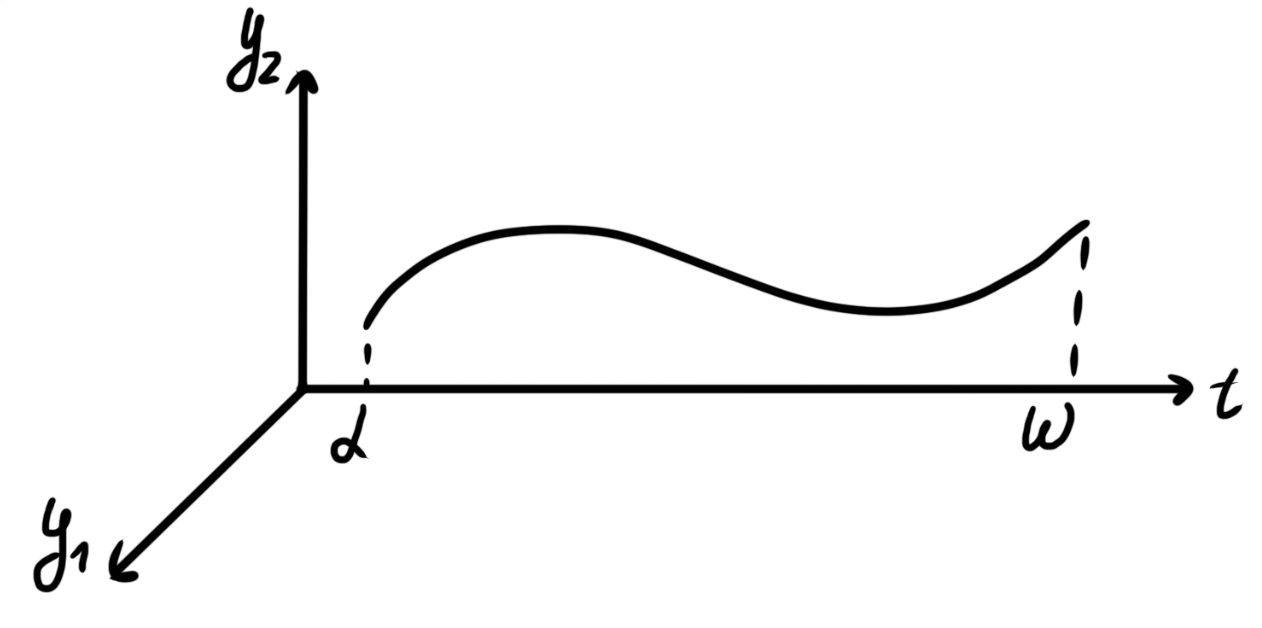
\includegraphics[width=0.6\textwidth]{/Users/vladbelousov/Desktop/Semestr_4-FP-NSU/ДфУ/Лекции_по_дням/image/45.png}
\end{center}

\textit{Интегральная кривая}  - график решения, то есть множество точек \( \{(t,y_1(t ),..., y_n(t)), t \in  (\alpha , \omega)\} \) 

\begin{center}
    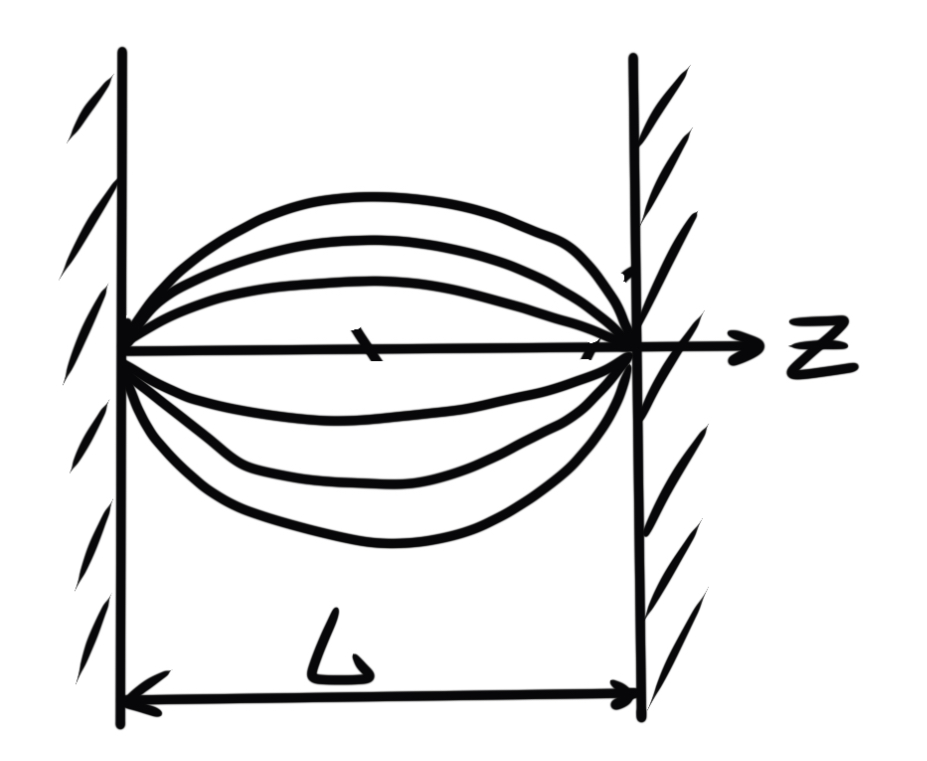
\includegraphics[width=0.4\textwidth]{/Users/vladbelousov/Desktop/Semestr_4-FP-NSU/ДфУ/Лекции_по_дням/image/46.png}
\end{center}

\textit{Фазовая траектория} - проекция интегральной кривой на пространство \( \{y_1, \ldots, y_n\} \), то есть множество точек \( \{(y_1, \ldots, y_n ) , t \in (\alpha , \omega)\} \) 

\textit{Фазовое пространство} - пространство \( \{y_1, \ldots, y_n\} \)  

Устойчивость нулевого решения: 

\begin{center}
    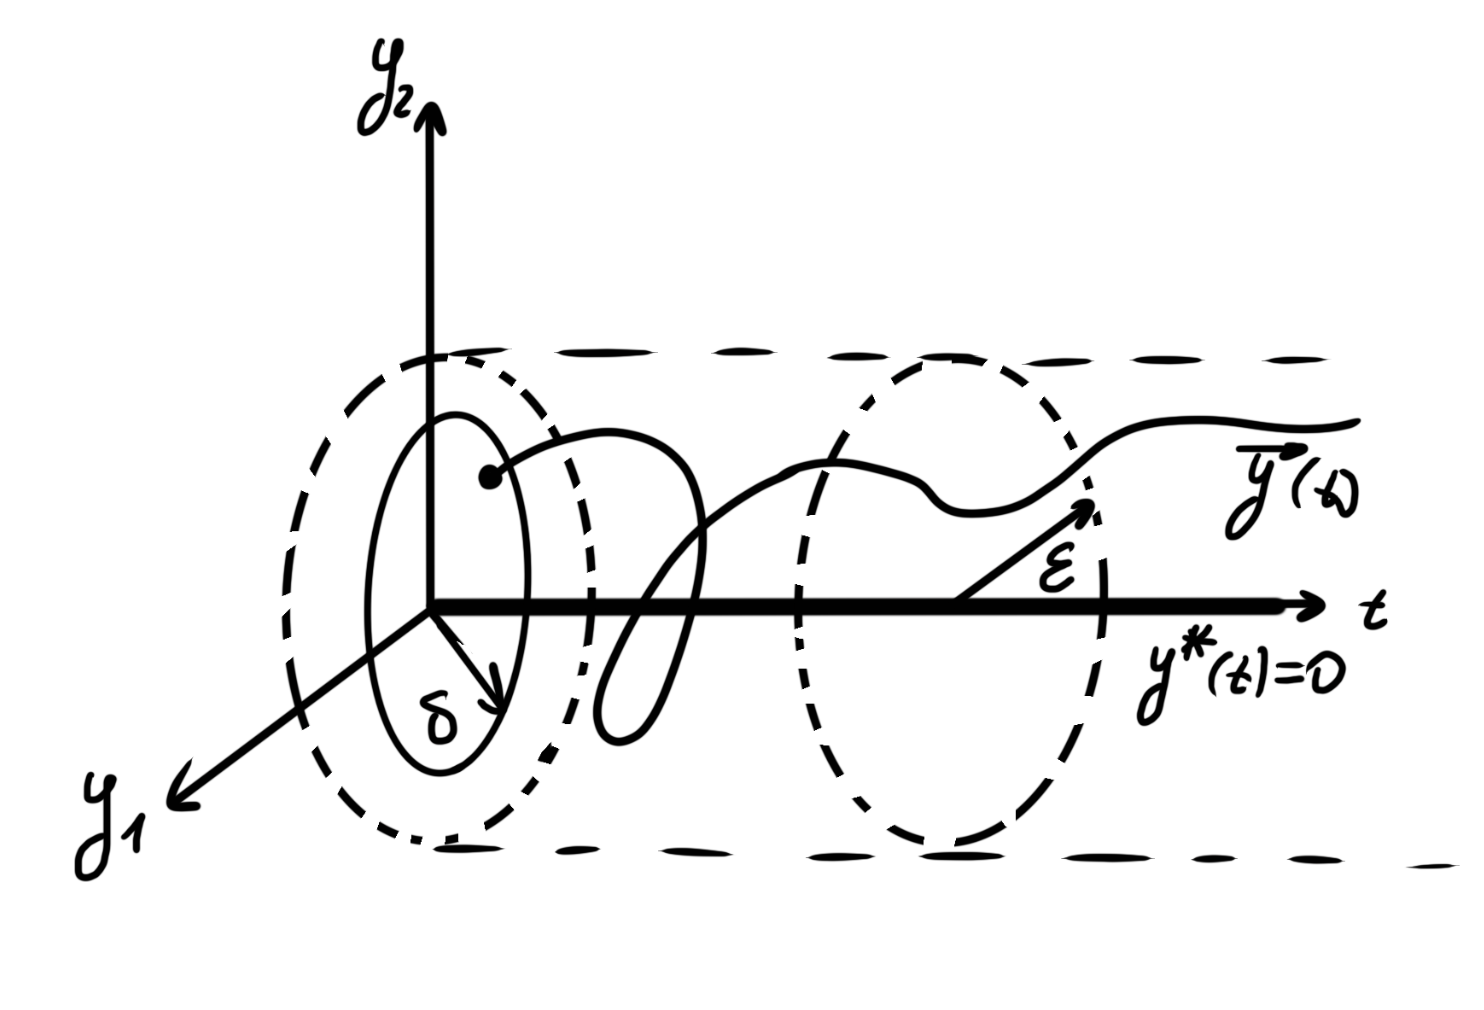
\includegraphics[width=0.6\textwidth]{/Users/vladbelousov/Desktop/Semestr_4-FP-NSU/ДфУ/Лекции_по_дням/image/47.png}
    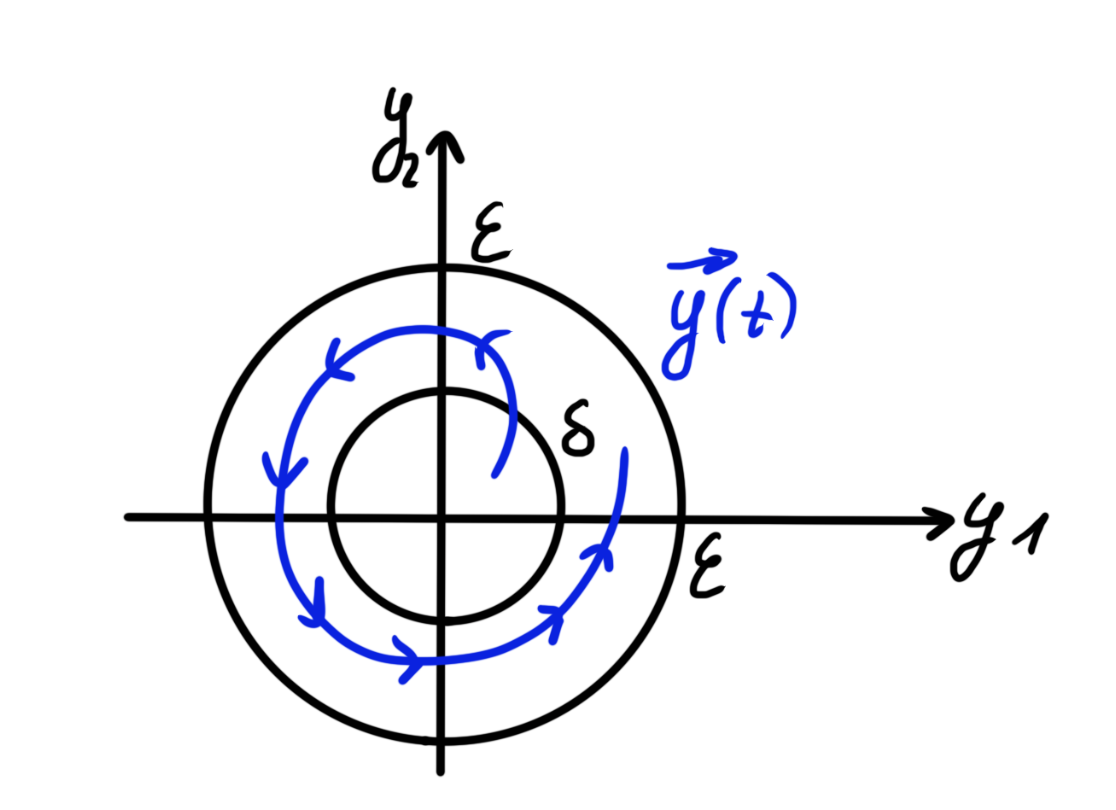
\includegraphics[width=0.3\textwidth]{/Users/vladbelousov/Desktop/Semestr_4-FP-NSU/ДфУ/Лекции_по_дням/image/48.png}
\end{center}

Предположим, что 

\begin{center}
    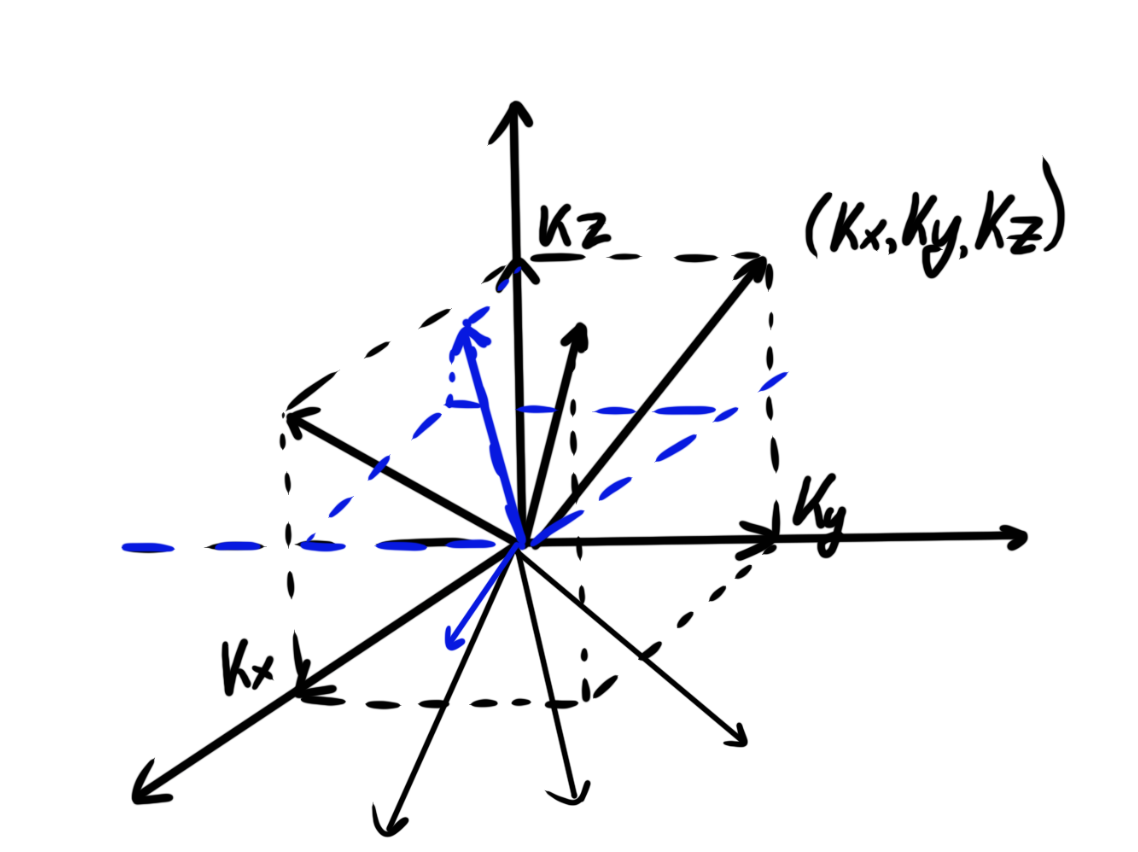
\includegraphics[width=0.55\textwidth]{/Users/vladbelousov/Desktop/Semestr_4-FP-NSU/ДфУ/Лекции_по_дням/image/49.png}
\end{center}

\[ \begin{pmatrix}
y_1(t)\\
y_2(t)
\end{pmatrix} \text{ - решение системы } \begin{cases}
y_1 ' = f_1 (y_1,y_2) \\ 
y_2' = f_2 (y_1 , y_2)
\end{cases} \] 

\begin{center}
    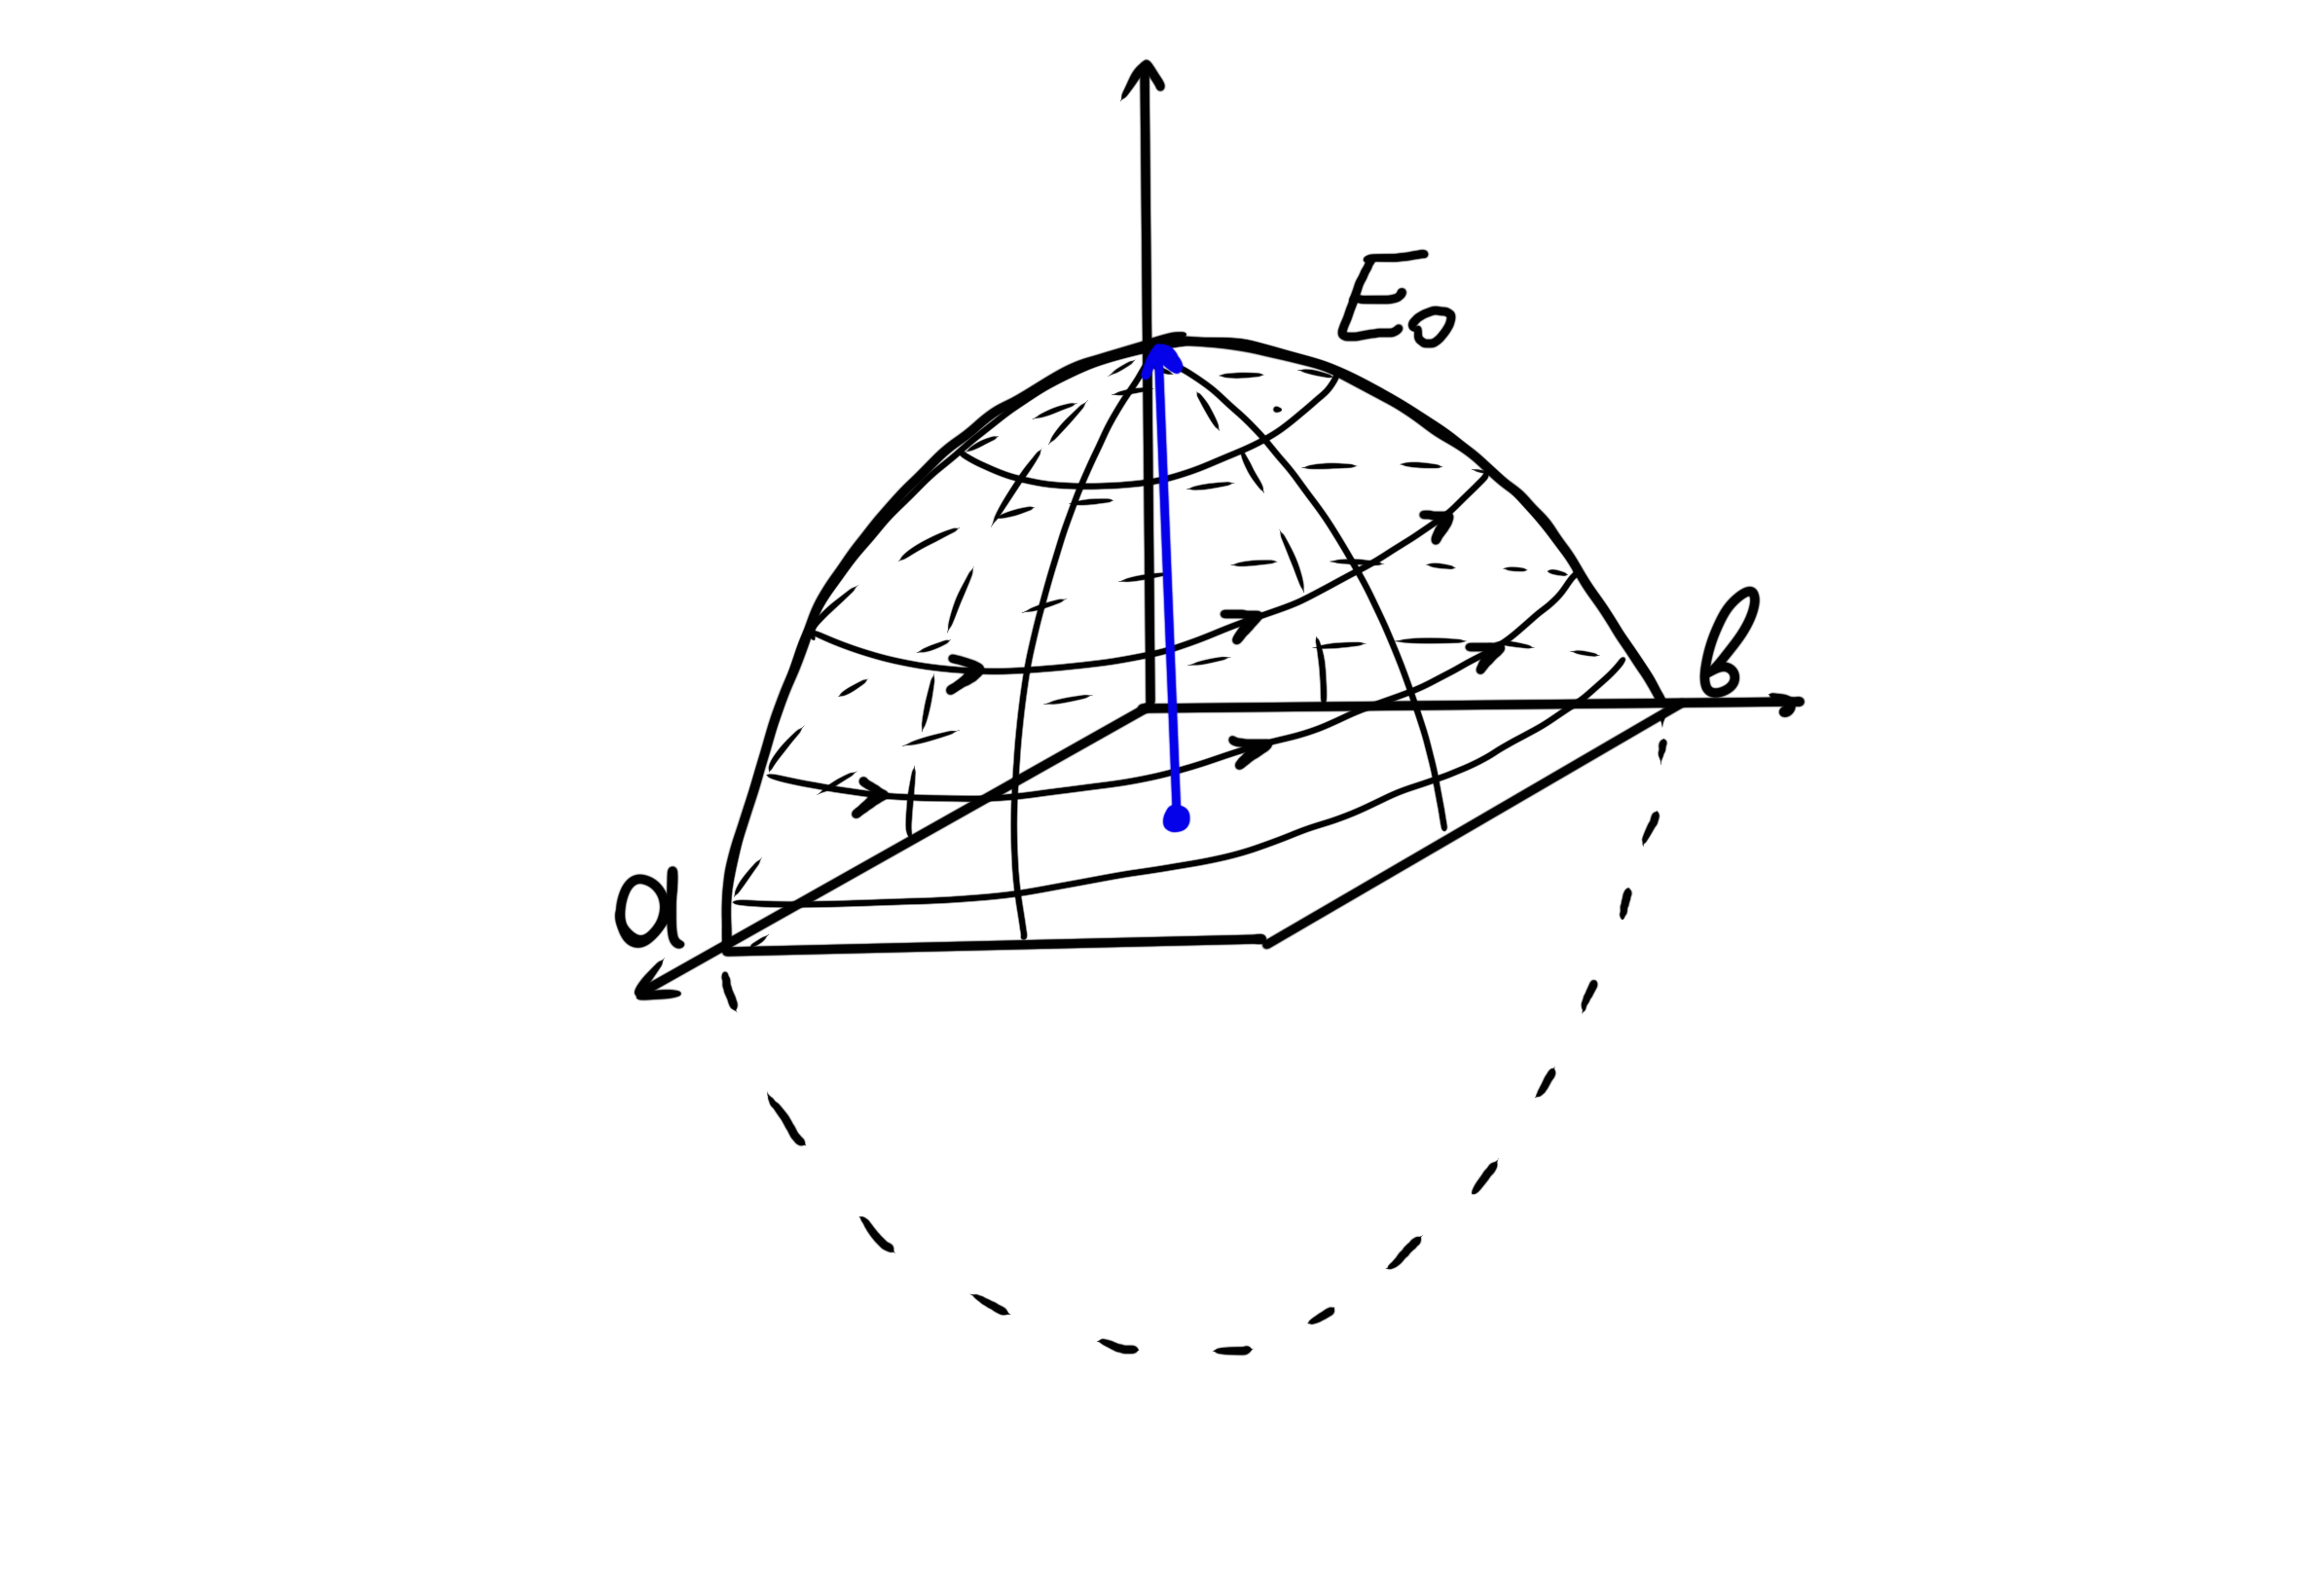
\includegraphics[width=0.3\textwidth]{/Users/vladbelousov/Desktop/Semestr_4-FP-NSU/ДфУ/Лекции_по_дням/image/50.png}
\end{center}

\[ V(y_1, y_2 ) = y_1 ^2 + y_2 ^2  = \varepsilon ^2  \] 

\[ \vec{n }  = \nabla V = \begin{pmatrix}
\displaystyle  \frac{ \partial  V }{\partial  y_1 }  \\[10pt]
\displaystyle  \frac{\partial  V }{\partial  y_2 } 
\end{pmatrix}= \begin{pmatrix}
2 y_1 \\
2 y_2 
\end{pmatrix} \] 

\( (\vec{\tau  } , \vec{n }  )< 0 \Leftrightarrow   \) угол между векторами \( \vec{\tau}  \) и \( \vec{ n}  \) от \( \displaystyle  \frac{\pi}{2 }  \)  до \( \pi \): 

\[ (\vec{\tau  } , \vec{n }  ) = \left(  \begin{pmatrix}
f_1 \\
f_2
\end{pmatrix}, \begin{pmatrix}
V _{y_1 } '  \\
V_{y_2 } ' 
\end{pmatrix} \right) = f_1 V_{y_1 } ' + f_2 V_{ y_2 } ' = f_1 2 y_1 + f_2 2 y_2 < 0   \] 

\begin{center}
    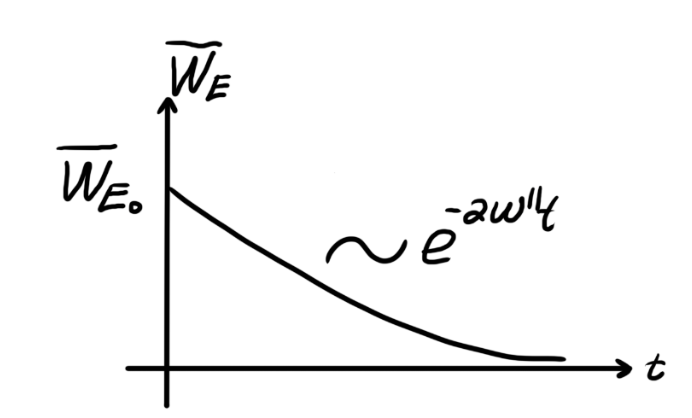
\includegraphics[width=0.4\textwidth]{/Users/vladbelousov/Desktop/Semestr_4-FP-NSU/ДфУ/Лекции_по_дням/image/52.png}
    \includegraphics[width=0.4\textwidth]{/Users/vladbelousov/Desktop/Semestr_4-FP-NSU/ДфУ/Лекции_по_дням/image/51.png}
\end{center}

\begin{definition}
    Функция \( V (\vec{y }  ) \), определенная  в шаре  \( \underbrace{ \{\left\lVert \vec{y }   \right\rVert < r\}}_{\Leftrightarrow  y_1 ^2 + ... + y_n ^2 < r ^2 } \), называется функцией Ляпунова для системы (1) если: 

    1) \( V (\vec{y } ) \in  C^1 (\left\lVert \vec{y }  \right\rVert < r ) \) 

    2) \( V (\vec{y }  ) > 0 \text{ }  \forall 0 < \left\lVert  \vec{ y}  (t) \right\rVert < r , \text{ }  V(\vec{ 0 } ) =0  \) 

    3) \( (\nabla V(\vec{y } ) , \vec{f } (\vec{y } ) ) \le  0 , \text{  }  \left\lVert \vec{y }  \right\rVert < r\)
\end{definition}

\begin{theorem}[Теорема Ляпунова об устойчивости по Ляпунову]
    Если для системы (1) существует функция Ляпунова, то нулевое решение устойчиво по Ляпунову.
\end{theorem}

Пример: Исследовать на устойчивость нулевое решение. 

\[ \begin{cases}
y_1 ' = - y_1  \\ 
y_2 ' = -y_2
\end{cases} \]

1 способ: 

\[ A= \begin{pmatrix}
-1 & 0\\
0 & -1
\end{pmatrix}, \text{ }  \lambda_{1,2} = -1  \text{ }  \mathrm{Re } \lambda_j <  0 \Rightarrow \text{нулевое решение асимптотически устойчиво }    \] 

2 способ: 

\[ V (y_1 , y_2 ) = y_1 ^2 + y_2 ^2  \] 

\[ \begin{aligned}
    1)& V \in  C^1 (\mathbb{R}) \\
    2)& V > 0 , \text{ }  (y_1,y_2 ) \neq (0,0 ) , \text{ }  V (0,0 ) = 0  \\
    3)& (\nabla V , f) = \left( \begin{pmatrix}
        2y_1    \\
        2y_2
        \end{pmatrix} , \begin{pmatrix}
        -y_1\\
        -y_2
        \end{pmatrix} \right)  = -2 y_1 ^2 - 2y_2 ^2 \le  0
\end{aligned} \] 

\( \Rightarrow \)  по Теореме Ляпунова нулевое решение устойчиво по Ляпунову.

\begin{center}
    \includegraphics[width=0.4\textwidth]{/Users/vladbelousov/Desktop/Semestr_4-FP-NSU/ДфУ/Лекции_по_дням/image/53.png}
\end{center}

\begin{theorem}[Теорема Ляпунова об асимптотической устойчивости]
    Пусть существует функция \( V(\vec{y} ) \), удовлетворяет условиям 1), 2), \( 3^*)  \text{ }  (\nabla V(\vec{y} ), \vec{f } (\vec{y } ))< 0\) при \( 0 < \left\lVert \vec{y }  \right\rVert < r \). Тогда нулевое решения \( \vec{y } ^* (t) =0  \) асимптотически устойчиво.
\end{theorem}

\begin{theorem}[Теорема Ляпунова об асимптотической неустойчивости]
    Пусть существует функция \( V(\vec{y} ) \) удовлетворяющее условиям 1), 2), \( 3^{**}) (\nabla V(\vec{y } ) , \vec{f } ( \vec{y } )) > 0  \) при \( 0 < \left\lVert  \vec{y }  \right\rVert < r \). Тогда нулевое  решение неустойчиво.
\end{theorem}
%%-------------------------------%%

% Закрытие документа, если файл компилируется отдельно
\ifdefined\mainfile
    % Если это основной файл, не нужно заканчивать документ
\else
    \end{document}
\fi
% Условная компиляция для самостоятельной работы
\ifdefined\mainfile
    % Если это часть основного файла, не добавляем начало и конец документа
\else
    \documentclass[12pt, a4paper]{report}
    \usepackage{/Users/vladbelousov/Desktop/Semestr_4-FP-NSU/Настройка/library}
    \usepackage[utf8]{inputenc} % Подключение поддержки UTF-8
    \begin{document}
\fi

%%-------------------------------%%

Вспомним \textbf{Определение 1.} 

Функция \( V (\vec{y }  ) \), определенная  в шаре  \( \underbrace{ \{\left\lVert \vec{y }   \right\rVert < r\}}_{\Leftrightarrow  y_1 ^2 + ... + y_n ^2 < r ^2 } \), называется функцией Ляпунова для системы (1) если: 

1) \( V (\vec{y } ) \in  C^1 (\left\lVert \vec{y }  \right\rVert < r ) \) 

2) \( V (\vec{y }  ) > 0 \text{ }  \forall 0 < \left\lVert  \vec{ y}  (t) \right\rVert < r , \text{ }  V(\vec{ 0 } ) =0  \) 

3) \( (\nabla V(\vec{y } ) , \vec{f } (\vec{y } ) ) \le  0 , \text{  }  \left\lVert \vec{y }  \right\rVert < r\)

\( 1) , 2) \Rightarrow  \) 

\begin{center}
    \includegraphics[width=0.4\textwidth]{/Users/vladbelousov/Desktop/Semestr_4-FP-NSU/ДфУ/Лекции_по_дням/image/54.png}
    \includegraphics[width=0.4\textwidth]{/Users/vladbelousov/Desktop/Semestr_4-FP-NSU/ДфУ/Лекции_по_дням/image/55.png}
\end{center} 

\( 3) \Rightarrow \) 

\begin{center}
    \includegraphics[width=0.6\textwidth]{/Users/vladbelousov/Desktop/Semestr_4-FP-NSU/ДфУ/Лекции_по_дням/image/56.png}
\end{center}

\begin{theorem}[Теорема Ляпунова об устойчивости]
    Пусть для системы (1) существует функция Ляпунова. Тогда нулевое решение \( \vec{y } ^* (t ) = 0 \) системы (1) устойчиво по Ляпунову.
\end{theorem}

\begin{proof} \(  \) 

    Надо доказать: 

    1) \( \vec{y }  ^* (t ) = 0 \) определенно от \( t_0     \)  до \( +\infty   \) (это верно)

    2) \( \exists  \Delta >0 \text{ }  \forall  \vec{y } (t_0 ) :  \left\lVert \vec{y }  (t_0) \right\rVert < \Delta \Rightarrow \vec{y } (t) \) определенно от \( t_0  \) до \( +\infty  \) 

    3) \( \forall  \varepsilon > 0 \text{ }  \exists  \delta > 0 \text{ }  \forall  \vec{ y }  (t_0 ) : \left\lVert \vec{y }  (t_0 ) \right\rVert < \delta \Rightarrow \left\lVert \vec{y } (t) \right\rVert < \varepsilon \text{ }  \forall  t \ge  t_0 \) 

    Пусть дано \( \varepsilon  > 0\): 

    \begin{center}
        \includegraphics[width=0.4\textwidth]{/Users/vladbelousov/Desktop/Semestr_4-FP-NSU/ДфУ/Лекции_по_дням/image/57.png}
    \end{center}

    Возьмем \(\displaystyle  \varepsilon_0 = \min  \left\{   \varepsilon , \frac{r}{2 } \right\} \). Обозначим \(\displaystyle  m(\varepsilon_0) = \min_{\left\lVert \vec{y }  \right\rVert = \varepsilon_0 } V(\vec{y }  )>0  \) 

    \begin{center}
        \includegraphics[width=0.4\textwidth]{/Users/vladbelousov/Desktop/Semestr_4-FP-NSU/ДфУ/Лекции_по_дням/image/58.png}
    \end{center}

    \[ M (\delta ) = \max _{\left\lVert \vec{y  }  \right\rVert \le  \delta } V(\vec{y }  )  \] 

    \begin{center}
        \includegraphics[width=0.7\textwidth]{/Users/vladbelousov/Desktop/Semestr_4-FP-NSU/ДфУ/Лекции_по_дням/image/59.png}
    \end{center}

    Выберем \( \delta  \) так, чтобы \( M(\delta ) < m (\varepsilon_0 ) \) 



    Утверждается, что \( \delta  < \varepsilon_0 \).

    От противного: пусть \( \delta \ge  \varepsilon_0  \). Тогда: 

    \[ m(\varepsilon_0 ) = \min _{\left\lVert \vec{y }  \right\rVert = \varepsilon_0} V(\vec{y } ) \le  \max _{ \left\lVert \vec{y }  \right\rVert = \varepsilon_0 }  V(\vec{y } ) \le  \max _{\left\lVert \vec{y }  \right\rVert \le  \varepsilon_0  } V(\vec{y} ) \overset{\delta \ge  \varepsilon_0}{\le } \max _{\left\lVert \vec{y }    \right\rVert \le  \delta } V(\vec{y }  ) = M(\delta )    \] 
    \begin{center}
        Противоречие \( \Rightarrow \delta < \varepsilon_0 \) \\
    \end{center} 

    Рассмотрим задачу Коши: 

    \[ \begin{aligned}
        \begin{cases}
            \displaystyle \frac{d}{dt }  \vec{y}  = \vec{f }  (\vec{y}  ) \\ 
            \vec{y } (t_0 ) = \vec{y }  _0
        \end{cases}
        \left\lVert \vec{y}  _0 \right\rVert <\delta 
    \end{aligned} \] 
    \( \Rightarrow \exists  !  \) непродолжаемое решение \( \vec{y}  (t ) \), определенное на открытом интервале \( \alpha , \omega ,\text{ }  t_0 \in  (\alpha , \omega ) , \text{  } \omega \le  + \infty  \) 

    Докажем, что \( \left\lVert \vec{y } (t) \right\rVert < \varepsilon_0 \text{ }  \forall   t \in [t_0 , \omega) \). 

    \begin{center}
        \includegraphics[width=0.7\textwidth]{/Users/vladbelousov/Desktop/Semestr_4-FP-NSU/ДфУ/Лекции_по_дням/image/60.png}
    \end{center}

    Пусть \( t^ * > t_0  \)  - первая точка, в которой \( \left\lVert \vec{y }  (t^* ) \right\rVert = \varepsilon_0 \), т.е \( \forall  t \in  [t_0,t^* ) : \left\lVert  \vec{y }  (t) \right\rVert < \varepsilon_0 \)  

    Воспользуемся условием 3) \( \nabla V (\vec{ y}  ) , \vec{f }  (\vec{y }  )  \le  0 , \text{ }  \left\lVert \vec{y }  \right\rVert < r\). 

    Возьмем решение \(\displaystyle  \vec{y}  (t ) , \text{ }  t \in  [t_0 , t^*] \Rightarrow \left\lVert \vec{y}  (t) \right\rVert \le  \varepsilon_0 \le \varepsilon_0 = \min \left\{   \varepsilon , \frac{r}{2 } \right\} \le  \frac{r}{2 }  <r \) 

    Возьмем \(\displaystyle  V (\vec{y }  (t ) ) \Rightarrow   \) 
    \[ \Rightarrow\frac{d}{dt }  V(\vec{y}  (t ) ) = \frac{d}{dt }  V (y_1(t ),..., y_n (t)) = \frac{\partial  V }{\partial  y_1 } (\vec{y}  (t ) )\underbrace{ \frac{d y_1(t )}{ dt }}_{f_1 (\vec{y} )}+ ...+ \frac{\partial  V }{\partial  y_n } (\vec{y }  (t )) \underbrace{\frac{d y_n(t )}{dt} }_{f_n (\vec{y} ) } =      \] 
    \[ = ( \nabla  V(\vec{y} (t )) , \vec{f }  (\vec{y}  (t ))) \le  0 \] 
 
    Получили \( \displaystyle  \frac{d}{dt }  V(\vec{y} (t )) \le  0 , \text{ }  t \in  [ t_0 , t^*] \)  


    \[ V(\vec{y}  (t ^* )) \le  V (\vec{y}  (t_0)) \tag{\(*  \) }\] 
    \[ V(\vec{y}  (t^* )) \ge  \min _{\left\lVert \vec{y}  \right\rVert = \varepsilon_0} V (\vec{y } ) = m(\varepsilon_0 )    \tag{\(**  \) }     \] 
    \[ V(\vec{y}  (t_0 ) )= V(\vec{y} _0  ) \le  \max _{\left\lVert \vec{y}  \right\rVert \le  \delta } V(\vec{y}  ) = M(\delta )  \tag{\(*  **\) } \] 

    \[ m(\varepsilon_0 ) \overset{(**)}{\le}  V(\vec{y }  (t^*)) \overset{(*)}{\le}  V(\vec{y }  (t_0)) \overset{(***)}{\le}  M(\delta )\text{ - противоречие.}  \] 
    \[ \Rightarrow \left\lVert \vec{y } (t) \right\rVert < \varepsilon_0 \text{  }  \forall  r \in  [ t_0 , \omega) \] 

    Мы доказали: 
    \[ \forall  \varepsilon > 0 \text{ }  \exists  \delta > 0 : \left\lVert \vec{y} (t_0) \right\rVert < \delta \Rightarrow \left\lVert \vec{y}  (t) \right\rVert < \varepsilon \text{ } \forall  r \in  [t_0 , \omega) \] 

    \begin{center}
        \includegraphics[width=0.7\textwidth]{/Users/vladbelousov/Desktop/Semestr_4-FP-NSU/ДфУ/Лекции_по_дням/image/61.png}
    \end{center}

    Пусть \( \omega < + \infty  , \text{  } \displaystyle  \lim_{t  \to \omega- 0} \vec{y } (t ) = \vec{y}  _{ \omega } \in  \mathbb{R} ^n    \) 

    Рассмотрим задачу Коши: 

    \[ \begin{aligned}
    \begin{cases}
        \displaystyle \frac{d}{dt }  \vec{y } = \vec{f }  (\vec{y }  ) \\
        \vec{y } (\omega ) = \vec{y } _{\omega} 
    \end{cases}
    \end{aligned} \] 
    \( \Rightarrow  \) по теореме Пикара \( \exists !  \) непродолжаемое решение \( \tilde{t } (t ) , \text{  }  t \in  (\tilde{\alpha } ,\tilde{ \omega }) , \text{ } \omega \in  (\tilde{ \alpha } , \tilde{ \omega})  \) 

    Рассмотрим функцию: 

    \[ \begin{aligned}
        z(t )=
     \begin{cases}
     y(t ) , \text{ }  t \in  [t_0 , \omega) \\
     \tilde{y } (t ) ,\text{ }  t \in  [\omega , \tilde{\omega})
     \end{cases}
     \text{  - продолжаемое решения }   y(t) \text{, т.е решение задачи Коши} 
    \end{aligned} \]  


\[ \begin{cases}
    \displaystyle  \frac{d}{dt }  \vec{y}  = \vec{f }  (\vec{y}  ) \\ 
    \vec{y }  (t_0 ) = \vec{y}  _0
    \end{cases} \] 
    
    Почему \( \displaystyle  \exists  \frac{d}{dt }  z(t ) \bigg | _{ t = \omega } ?   \) 
    
    \[ \frac{d}{dt }  z(t ) \bigg | _{t = \omega  -0 }  = \vec{f }  (\vec{y } ) | _{t = \omega - 0 } = \vec{f }  (\vec{y } _{\omega} )   \] 
    \[ \frac{d}{dt }  z(t ) \bigg | _{t = \omega  +0 }  = \vec{f }  (\vec{y } ) | _{t = \omega +0 } = \vec{f }  (\vec{y } _{\omega} )   \] 
    
    Противоречие с тем, что \( \vec{y } (t) \) - непродолжаемое решение \( \Rightarrow \omega = + \infty  \Rightarrow  \) доказан пункт 3). 
    
    
    2) Возьмем \( \displaystyle  \varepsilon = \frac{r ' }{2 } \Rightarrow \exists  \delta \left(  \frac{r}{2 }  \right) \Rightarrow  \Delta  = \delta \left( \frac{r}{2 }  \right) \Rightarrow  \) доказан пункт 2). 
    
    \[  \Rightarrow \vec{y } ^* (t ) = 0  \text{ устойчиво по Ляпунову} \] 
\end{proof}

\begin{theorem}[Теорема Ляпунова об асимптотической устойчивости] 
    Пусть функция \( V(\vec{y} ) \)  такая, что выполнено условие 1), 2), \( 3^*) (\nabla V (\vec{y }  ,\vec{f }  (\vec{y } ))) < 0  ,\text{ }  0 < \left\lVert  \vec{y }  \right\rVert < r  \). Тогда \( \vec{y } ^* (t ) = 0 \) системы (1) асимптотически устойчиво.

    Без доказательства.
\end{theorem}

\begin{theorem}[Теорема Ляпунова о неустойчивости]
    Пусть существует функция \( V(\vec{y } ) \), удовлетворяющее условиям 1), 2),  \(3^{** } ) (\nabla V (\vec{y}  ) \vec{f } (\vec{y } ) ) >0 , \text{ }  0 < \left\lVert \vec{y }  \right\rVert < r  \). Тогда \( \vec{y } ^* (t ) = 0 \)   неустойчиво. 
\end{theorem}

\begin{proof} \(  \) 

    От противного: пусть \( \vec{y } ^* (t)  = 0 \) устойчиво по Ляпунову, в частности, \( \forall  \varepsilon > 0 \text{ }  \exists  \delta > 0  \text{ }  \forall  \vec{y } (t_0 ) : \left\lVert  \vec{y}  (t_0 ) \right\rVert < \delta \Rightarrow \left\lVert \vec{y}  (t) \right\rVert < \varepsilon \text{ } \forall  t > t_0 \) 

    Возьмем \( \displaystyle  \varepsilon = \frac{r}{2 }  \Rightarrow \exists  \delta \left( \frac{r}{2 }    \right) : \left\lVert \vec{y} (t_0 ) \right\rVert < \delta \left( \frac{r}{2}  \right) \Rightarrow \left\lVert \vec{y} (t ) \right\rVert < \frac{r}{2 }  <r  \text{ }  \forall  t \ge  t_0 \) 

    \begin{center}
        \includegraphics[width=0.4\textwidth]{/Users/vladbelousov/Desktop/Semestr_4-FP-NSU/ДфУ/Лекции_по_дням/image/62.png}
    \end{center}

    Рассмотрим задачу Коши: 

    \[\begin{aligned}
        \begin{cases}
            \displaystyle \frac{d}{dt } \vec{y}  = \vec{f } (\vec{y} ) \\
            \vec{y } (t_0) = \vec{y } _0
        \end{cases} 
        , \left\lVert \vec{y}  _0 \right\rVert < \delta \left( \frac{r}{2 }  \right) , \text{ }  \kern-0.8cm\underbrace{\vec{y } _0}_{\vec{y}  (t ) \neq 0 ,\text{ }  \forall  t \ge  t_0} \kern-0.8cm \neq \vec{0} \Rightarrow  \left\lVert \vec{ y } (t ) \right\rVert < \frac{r}{2 }  \text{ }  \forall  t \in  [ t_0 , + \infty ) 
    \end{aligned}\] 

    \begin{center}
        \includegraphics[width=0.7\textwidth]{/Users/vladbelousov/Desktop/Semestr_4-FP-NSU/ДфУ/Лекции_по_дням/image/63.png}
    \end{center}

    \[ \begin{aligned}
    \begin{cases}
    \displaystyle  \frac{d}{dt }  \vec{y}  = \vec{f } (\vec{y} ) \\ 
    \vec{y } (\tilde{t } ) = 0
    \end{cases}
    \Rightarrow \vec{y } ^* (t ) = 0 \text{ - решение.} 
    \end{aligned} \] 


\( 3) \Rightarrow \displaystyle  \frac{d}{dt }  V(\vec{y}  (t))  = (\nabla V(\vec{y }  (t ) ) , \vec{f }  (\vec{y}(t) )) > 0 ,\text{ }  t \ge  t_0 \) 

\[ V(\vec{y } (t )) > \underbrace{V (\vec{y } (t_0))}_{= \alpha > 0} ,\text{ } t> t_0 \] 
\[ V(\vec{y}  (t) ) > \alpha , \text{ }  t \ge  t_0 \] 

Рассмотрим множество \( \displaystyle  \underbrace{\left\{   \vec{ y}  : \mathbb{R} ^2 : \left\lVert \vec{y}  \right\rVert \le  \frac{r}{2 }  , \text{ }  V(\vec{y } ) \ge  \alpha \right\}}_{P}\)- компакт, \( \forall  t \ge  t_0 , \text{ }  \left\lVert \vec{y}(t)  \right\rVert \in  P , \text{ } \vec{0 }\text{ }  \cancel{\in  } \text{ } P\)  

Рассмотрим: 

\[ \min_{\vec{y } \in  P } (\nabla V (\vec{y}  ) , \vec{f } (\vec{y} )) = \gamma > 0   \] 
\[ \frac{d}{dt  } V(\vec{y }(t)  ) = (\nabla V(\vec{y} (t)) , \vec{f }  (\vec{y } (t)))\overset{\vec{y} (t) \in  P}{ \ge}  \gamma > 0 \text{ }  \bigg | \int_{t_0}^{t}     \] 
\[ \int_{t_0}^{t } \frac{d}{ds }  V(\vec{y} (s )) ds \ge  \int_{t_0}^{t } \gamma ds    \] 
\[ V(\vec{y } (t )) \ge  V(\vec{y } (t_0)) + \underbrace{\gamma (t -t_0 )}_{\to  \infty } , \text{ }  \forall  t \ge  t_0 \text{ при } t \to  +\infty \] 
\[ \Rightarrow V(\vec{y} (t)) \to  \infty  \] 

\[ \left\lVert  \vec{y} (t) \right\rVert \le  \frac{r}{2 }  \] 
\[ V(\vec{y} (t )) \le  \max _{\left\lVert  \vec{y}  \right\rVert \le  \frac{r}{2 } } V(\vec{y} ) < + \infty   \] 
\[ \text{Противоречие.}  \] 

\[ \Rightarrow \vec{y } ^* (t ) = 0  \text{ неустойчиво } \] 

\end{proof}

Пример: Исследовать на устойчивость нулевое решение: 

\[ \begin{aligned}
    \begin{cases}
        y_1 ' =y_2 + \alpha y_1 ^3  \\ 
        y_2 ' = -y_1 \alpha y_2 ^3
    \end{cases} 
    \begin{cases}
    y_1^* (t ) = 0 \\
    y_2^* (t ) = 0
    \end{cases}
    \text{ - решение.} 
\end{aligned}\] 


\[ V(y_1,y_2 ) = a y_1 ^{2n }  + b y_2 ^{2 m }  \text{ }  (a,b > 0 \text{ }  m  , n \in \mathbb{N}) -\text{ выполнены } 1),2) \] 
, где \( a , b > 0 , \text{ }  n , m \in  \mathbb{N} \) 

\[ (\nabla V ,f )  = \left( \begin{pmatrix}
2a  n y^{2n -1 }_1 \\
2b  m y^{2m - 1 }  _2 
\end{pmatrix} , \begin{pmatrix}
y_2 + \alpha y_1 ^3 \\
-y_1+ \alpha y_2 ^3
\end{pmatrix}\right) =  \]  
\[ =2n a y_1 ^{2n -1 }  y_2 + 2n a y_1 ^{2n -1 }  \alpha y_1 ^3  + 2 bm y_2 ^{2m - 1 }  +2 m b y^{2 m- 1 } y_2 ^3\] 




%%-------------------------------%%

% Закрытие документа, если файл компилируется отдельно
\ifdefined\mainfile
    % Если это основной файл, не нужно заканчивать документ
\else
    \end{document}
\fi
% Условная компиляция для самостоятельной работы
\ifdefined\mainfile
    % Если это часть основного файла, не добавляем начало и конец документа
\else
    \documentclass[12pt, a4paper]{report}
    \usepackage{/Users/vladbelousov/Desktop/Semestr_4-FP-NSU/Настройка/library}
    \usepackage[utf8]{inputenc} % Подключение поддержки UTF-8
    \begin{document}
\fi

%%-------------------------------%%

\[  = 2n a y_1 ^{ 2n -1 }  y_2 + \underbrace{\alpha 2 n a y_1 ^{2n + 2 }}_{(*)}  +\underbrace{ \alpha 2 m b y_2 ^{ 2m + 2 }}_{(*)}  - 2m b y_1 y_2^{2m -1 }  \] 
, где \( (*): \begin{aligned}
>0 , \text{ }  \alpha > 0 \\ 
< 0 , \text{ }  \alpha < 0
\end{aligned} \) 

Занулим член с без явного знака: \( \begin{aligned}
m =n =1 \\ 
a = b  =1 
\end{aligned} \) 

\[ \Rightarrow V( y_1 , y_2 ) =  y_1 ^2 + y_2 ^2  \] 
\[ (\nabla V , f ) = 2 \alpha y_1 ^4 + 2 \alpha y_2^4  \] 

Рассмотрим случаи: 

- \(\alpha > 0 \Rightarrow  \) по Теореме 3 нулевое решение не устойчиво.

- \( \alpha < 0 \Rightarrow  \) по Теореме 2 нулевое решение асимптотически устойчиво.

- \( \alpha = 0 \Rightarrow \) по Теореме 1 нулевое решение устойчиво по Ляпунову. 

\[ \alpha = 0 : \begin{aligned}
    \begin{cases}
        \dot{y } _1 = y_1 \\ 
        \dot{ y } _2 = y_2
    \end{cases} 
    \quad  A \begin{pmatrix}
    0 & 1\\
    -1 & 0
    \end{pmatrix}
    , \lambda_{1,2}  = \pm  i 
\end{aligned}\] 

\section{Функция Ляпунова для линейных систем. Матричное уравнение Ляпунова}

\[ \frac{d}{dt }  \vec{y }  = A \vec{y }  \tag{1} \] 
, где \( A - (n \times  n ) \) постоянная. \( \vec{y } ^* (t ) = 0  \) - решение. 

\textbf{Матричное уравнение Ляпунова:} 

\[ HA + A^{ * }  H = -C \tag{2} \] 
, где \( A, H , C  \) - матрицы \( (n \times  n) \) постоянные. \\

Дано: \( A, C \) 

Найти: \( H - ? \) \\

Пример: \( \begin{pmatrix}
-1 & 1 \\
0 & -1
\end{pmatrix} , \text{ }  C = \begin{pmatrix}
1  & 0\\
0  & 1
\end{pmatrix} , \text{ }  H - ? \) 

\[ H = \begin{pmatrix}
h_{11}   & h_{12}\\ h_{21} & h_{22}
\end{pmatrix} \] 

\[ \begin{pmatrix}
- h_{11} & h_{11} - h_{12}\\
- h_{21} & h_{21} - h_{22}
\end{pmatrix} - \begin{pmatrix}
-1 & 0 \\
1  & -1
\end{pmatrix} \begin{pmatrix}
h_{11} & h_{12}\\
h_{21} & h_{22}
\end{pmatrix} = \begin{pmatrix}
-1 & 0 \\
0 & -1
\end{pmatrix}\] 

\[ \begin{pmatrix}
- 2 h_{11} & h_{11} - 2 h_{12}\\
h_{11} - 2 h_{21} & h_{12} - 2 h_{22} + h_{12}
\end{pmatrix} = \begin{pmatrix}
-1  & 0 \\
0 & -1
\end{pmatrix} \] 

\[ h_{11} = 2h_{12} = 2h_{21}  \] 
\[ h_{11} = \frac{1}{2 }  \Rightarrow h_{12} = h_{21} = \frac{1}{4}  \] 
\[ 2 h_{22} = h_{12} + h_{21} + 1 = \frac{3}{2}  \] 
\[ h_{22} = \frac{3}{4}  \] 

\[ H = \begin{pmatrix}
\frac{1}{2 }  & \frac{1}{4} \\
\frac{1}{4}  & \frac{3}{4} 
\end{pmatrix} \] 

\begin{theorem}
    Пусть дано \( C = C^* > 0\), то есть \( \forall  \vec{v }  \neq  0 : (C \vec{v }  , \vec{v  }  ) > 0   \). Пусть \( \exists H : H = H ^* > 0  \) - решение матрицы уравнения Ляпунова (2). Тогда: нулевое решение \( y^* (t) = 0 \) системы (1) асимптотически устойчиво.
\end{theorem}

\begin{proof} \(  \) 

    Рассмотрим функцию \( V(\vec{y} )  = (H  \vec{y }  , \vec{y  })  \text{ }  \vec{ y }  \in  \mathbb{R} ^2  \) 

    1) \( V (\vec{y } )  \in  C^* (\mathbb{R} ^n )  \) 

    \[ V (\vec{ y }  ) = \sum_{i, j =1} ^n h_{i j } y_i y_j \in  C^1 (\mathbb{R}^n) \] 

    2) \(  V(\vec{0 }  ) = ( H \vec{0 }  , \vec{0 }  ) = 0  \) 

    \[ V (\vec{ y}  ) = (H \vec{ y}  , \vec{y} ) > 0 \text{ при } \vec{y }  \neq  \vec{0 }  \text{ так как }  H = H^* > 0    \] 

    \[ \frac{d}{dt } \vec{y }  = A \vec{y }  \text{ }  A \text{ - постоянная} \tag{1 } \] 

    \[ HA + A ^* H   =  -C \text{ - матричное уравнение Ляпунова} \tag{2} \] 

    3) Проверим, что \( (\nabla V (\vec{ y}  ) , A \vec{ y}  ) < 0  \) при \( \vec{ y }  \neq  \vec{ 0 }  \) 

    Пусть \( \vec{ y} ( t) \) - решение задачи Коши: \( \displaystyle  \begin{cases}
    \displaystyle \frac{d}{dt }  \vec{y }  =A \vec{ y}  \\ 
    \displaystyle  \vec{ y} (0 ) = \vec{ y }  _0 
    \end{cases} \) 

    Возьмем \( V (\vec{ y}  (t)) \): 

    \[ \frac{d}{dt }  V(\vec{ y}  (t))  = \frac{d}{dt }  V(y_1(t ) ,..., y_n(t))  = \frac{\partial}{\partial  y_1 } V(y_1 ,...,y_n ) \frac{d y_1 }{dt } + ... + \frac{\partial  }{\partial  y_n } V(y_2 , ... ,y_n ) \frac{\partial  y_n }{\partial  t} = (\nabla V , A \vec{ y} )    \] 

    С другой стороны, 

    \[ \frac{d}{dt }  V (\vec{ y}  (t ) ) = \frac{d}{dt }  (H \vec{ y} (t ) , \vec{ y}  (t ))  = \left( H \frac{d}{dt }  \vec{ y}  (t ) ,\vec{ y}  (t ) \right)+ \left( H \vec{ y}  (t ) ,\frac{d}{dt }  \vec{ y}  (t ) \right) = (HA \vec{ y}, \vec{ y}  ) + (H \vec{ y}  , A \vec{ y}  ) = \] 
    \[ = (H A \vec{y } , \vec{ y}   ) + (A ^* H \vec{ y}  , \vec{ y}  ) = (\underbrace{(H A + A ^* H )}_{= -C} \vec{ y }  , \vec{y}       )= - (C \vec{ y}   , \vec{ y} )\] 

    \[ \Rightarrow (\nabla V, A \vec{ y}  (t ) ) = - ( C \vec{ y } (t) , \vec{ y} (t )) , \text{ }  \forall  t \in  \mathbb{R}^2  \] 
    \[ t = 0 : (\nabla V , A \vec{ y}  _0 ) = -(C \vec{ y}  _0 , \vec{ y } _0 )  , \text{ }  \forall  y_0 \in  \mathbb{R}^{n }  , \text{ }  \vec{ y_0  } \neq  \vec{ 0 }    \] 

    Так как \( C = C^* > 0  \), то \( (\nabla V (\vec{ y } _ 0 ) , \vec{f }  (\vec{ y }  _0 )) < 0  \) при \( \vec{ y } _ 0 \neq  \vec{ 0}  \Rightarrow \vec{ y } ^* (t ) = 0 \) - асимптотически устойчиво. 

\end{proof}

\begin{theorem}
    Пусть \( \lambda_1(A ) , ..., \lambda_n (A )  \) - собственные значения матрицы \( A \). Пусть \( \forall  \lambda_j (A ) \text{ } Re \lambda_j (A ) < 0  \). Тогда: 

    1) \( \forall   \) матрицы \(  C \text{ }  \exists ! H  \) - решение матр. уравнения (2)

    2) если \( C = C^*  \), то \( H = H^* \) 

    3) если \( C = C^*  \), то \( H =H^* > 0 \) 
\end{theorem}

\begin{proof} \(  \) 

    \[ e^{ t A ^* }  \cdot   | \text{ }  H A + A ^* H = -C \text{ }  | \cdot e^{tA }   \] 
    \[ e^{t A ^* }  H \underbrace{A e^{tA }}_{\frac{d}{dt }  e^{tA }= }  + \underbrace{e^{t A ^* }  A ^* }_{=\frac{d}{dt } e^{rA ^*}  }H e^{t A }  = - e^{r A ^* }   C e^{t A }  \] 
    \[ \frac{d}{dt } (e^{ t A^* } H e^{tA }   ) = -e^{t A^* } C e^{ tA }  \text{ } |\cdot \int_{0 }^{s} , s>0    \] 
    \[ \int_{0}^{s }  \frac{d}{dt } (e^{ t A^* } H e^{tA }   ) dt = - \int e^{t A^* } C e^{ tA } dt    \] 
    \[ e^{s A ^* }  H e^{ s A }  - H = \int_{- }^{s }  e^{t A ^* }  C e^{t A }  dt  \] 
    \[ A = T I T^{-1 }  \] 
    \[ e^{tA }  = T e^{ t I }  T^{-1 }  \] 
    \[ e^{t I }  = \begin{pmatrix}
    e^{\lambda_1 t }  &  & \\
    \vdots & \ddots & \frac{ t^ k e^{ \lambda_i t } }{ k!}  \\[10pt]
    0 & \cdots   & e^{ \lambda_n t } 
    \end{pmatrix}  \xrightarrow{t \to  + \infty  } 0   \] 

    При \( s \to  + \infty  \): 

    \[ H = \int_{0}^{\infty}  e^{ t A ^* }  C e^{tA }  d t \text{ - интеграл Ляпунова} \tag{3} \]
    
    2) Пусть \( C = C^* :  \) 

    \[ H^* = \left( \int_{0}^{\infty} e^{ t A ^* }  C e^{t A }  dt  \right) ^* = \int_{0 }^{\infty}\underbrace{     (e^{t A } )^*}_{e^{t A ^*} }\underbrace{ C ^* }_{C}\underbrace{ (e^{t A ^* } )^*}_{e^{tA } } dt = H\] 

    3) Пусть \( C = C^* > 0  \), то есть \(  \forall  \vec{v }  \neq  \vec{ 0}  : (C \vec{v } , \vec{v }         ) >0  \): 

    \[ (H \vec{ v }  ,\vec{ v }  ) = \left( \int_{0}^{\infty} e^{t A ^* }  C e^{tA }  dt \vec{v }  ,\vec{v }   \right) = \left( \int_{0}^{\infty} e^{tA^* }  C e^{tA } \vec{ v }  dt , \vec{ v }   \right) = \int_{0}^{\infty} (e^{tA ^* }  C e^{tA }  \vec{v } ,\vec{ v } ) = \] 
    \[ = \int_{0}^{\infty} ( C \underbrace{e^{tA }  \vec{v }}_{ w(t ) \neq  0 }   ,\underbrace{e^{tA }  \vec{ v }}_{w (t ) \neq  0}   ) dt > 0  \] 

\end{proof}


\begin{theorem}
    Следующие условия эквиваленты: 
    
    1) \( \vec{ y } ^* (t ) = 0  \) - решение системы (1) \( \displaystyle  \frac{d}{dt }  \vec{ y}  = A \vec{ y}   \) асимптотически устойчиво; 

    2) \( \forall  \lambda_j (A ) \text{ }  Re \lambda_j (A )< 0  \); 

    3) \( \forall   \) матрицы \( C = C^* >0 \text{ }  \exists  ! \text{ }  H = H^* > 0  \) - решение матричного уравнения (2) \( HA + A^* H = - C  \) 

    \[ \begin{aligned}
    1) & \Leftrightarrow 2) \text{ - было } \\
    2) &\Rightarrow  3) \text{ - следует из Теоремы 2 } \\
    3) &\Rightarrow 1) \text{ - следует из Теоремы 1} 
    \end{aligned} \] 
\end{theorem}

\section{Исследование решений на устойчивость по первому приближению}

\[ \frac{d}{dt }  \vec{ y}  = \vec{ f }  (\vec{ y} ) \tag{1} \] 
, где \( \vec{ f }  \in  C ^1 (\mathbb{D} ) ,\) \( \vec{  y} ^{* }  (t ) = 0  \) - решение \( \Rightarrow   \vec{ f }  (\vec{ 0 } ) = \vec{0 } \) 

Разложим правую часть уравнения \( (1) \) в ряд Тейлора: 

\[ \frac{d}{dt }  \vec{ y}  = \vec{ f }  (\vec{ 0}  ) + \underbrace{\frac{ \partial  \vec{ f } }{\partial  \vec{ y}  } }_{(*)}(0 ) \vec{ y } + o(\left\lVert \vec{ y}  \right\rVert)   \] 
, где \( (*) \) - матрица \( n \times  n  = A  \). \( o(\left\lVert  \vec{ y}  \right\rVert)  \), то есть \( \displaystyle \lim_{\left\lVert  \vec{y }  \right\rVert \to 0 } \frac{o \left\lVert \vec{y }  \right\rVert}{\left\lVert  \vec{ y }  \right\rVert } = 0   \quad  (2)\) 

\[ \frac{d}{dt } \vec{ y}  = A \vec{ y}  + o (\left\lVert  \vec{ y }  \right\rVert) \] 

\begin{theorem}[Теорема Ляпунова об устойчивости по первому приближению] \(  \) 

    1) Если \( \forall  \lambda_j (A ): Re \lambda_j (A ) < 0 \Rightarrow \vec{ y} ^* (t ) = 0  \)  асимптотически устойчиво. 

    2) \( \exists  \lambda_k (A ) : Re \lambda_k >0 \Rightarrow \vec{ y } ^* (t ) = 0  \) - неустойчиво.
\end{theorem}

%%-------------------------------%%

% Закрытие документа, если файл компилируется отдельно
\ifdefined\mainfile
    % Если это основной файл, не нужно заканчивать документ
\else
    \end{document}
\fi
%Май
% Условная компиляция для самостоятельной работы
\ifdefined\mainfile
    % Если это часть основного файла, не добавляем начало и конец документа
\else
    \documentclass[12pt, a4paper]{report}
    \usepackage{/Users/vladbelousov/Desktop/Semestr_4-FP-NSU/Настройка/library}
    \usepackage[utf8]{inputenc} % Подключение поддержки UTF-8
    \begin{document}
\fi

%%-------------------------------%%

\begin{proof} \(  \) 

    1) Дано: \( \forall  \lambda_j (A ) \text{ }  Re \lambda_j (A ) < 0 \). Пусть \( C  = E \), \(  E = E^* > 0 \). Тогда по Теореме 3 \( \exists  ! H = H^* > 0  \) - решение матричного уравнения \( HA + A ^* H = - E . \) 

    Рассмотрим функцию \( V(\vec{ y} ) = ( H \vec{ y}  , \vec{ y} ) \). Покажем, что \( V(\vec{ y} ) \) - функция Ляпунова: 

    \( \kern+0.5cm  \) 1. \( V(\vec{ y} ) = (H \vec{ y}  , \vec{y }  ) \in  C ^1 (\left\lVert  \vec{ y}  \right\rVert < r ) \), где \( r  \) - любое; 

    \( \kern+0.5cm  \) 2. \( V(\vec{ 0}  ) = (H \vec{ 0}  , \vec{ 0 } ) = 0 , \text{ }  V (\vec{ y}  ) = (H \vec{ y}  , \vec{ y}  ) > 0 \) при \( \vec{ y }  \neq  \vec{0 }  \), так как \( H = H ^*>0 \) 

    \( \kern+0.5cm  \) 3. \(( \nabla V \vec{y }  , \vec{f }  (\vec{ y}  )) < 0  \) - ? 

    Пусть \( \vec{ y }  (t )  \) - решение \( \begin{cases}
    \displaystyle  \frac{d}{dt }  \vec{ y}  = \vec{f }(\vec{ y} ) = A  \vec{ y}  + \vec{g }  (\vec{ y} )  \\ 
    \vec{y }  (t_0 )= \vec{ y}  _0 \neq  \vec{ 0} 
    \end{cases} \) 

    , где \( \vec{ g } (\vec{ y} ) = o (\left\lVert \vec{y}  \right\rVert) \) 

    \[ \frac{d}{dt }  V (\vec{ y} (t )) = \frac{d}{dt }  V (y_1 (t ) ,..., y_n (t )) = \frac{\partial  V }{\partial  y_1 } (\vec{ y }  (t ) ) \underbrace{\frac{d y_1 (t )}{dt }}_{f_1 (\vec{ y}  (t))} + ...+  \frac{\partial  V }{\partial  y_n } (\vec{ y}  (t ))\underbrace{ \frac{d y_n (t )}{dt }}_{f_n (\vec{y } (t))}   = (\nabla V (\vec{ y}  (t )) , \vec{ f }  (\vec{ y }  (t)))\]  

    С другой стороны: 

    \[ \frac{d}{dt }  V (\vec{ y}  (t )) = \frac{d}{dt }  (H \vec{ y}  (t ) , \vec{ y}  (t )) = \bigg( H\underbrace{ \frac{d}{dt } \vec{ y}}_{\vec{ f   } (\vec{ y}  (t)) }  (t ), \vec{ y}  (t ) \bigg) + \bigg(  H \vec{ y}  (t ) , \underbrace{\frac{d}{dt }  \vec{ y }  (t)}_{\vec{ f } (\vec{ y}  (t))} \bigg) =\] 
    \[ = \bigg(  H (A \vec{ y}  (t ) + \vec{ g }  (\vec{ y}  (t ))) , \vec{ y}  (t ) \bigg)  + \bigg(  H \vec{ y}  (t ) , A \vec{ y}  (t ) + \vec{ g }  (\vec{ y }  (t)) \bigg)  = \] 
    \[  = (H A \vec{ y}  (t ) , \vec{ y}  (t ) ) + (H \vec{ g }  (\vec{ y }  (t ))) + (H \vec{ y } (t ) , A \vec{ y}  (t )) + ( H \vec{ y}  (t ) , \vec{ g }(\vec{ y}  (t)) ) = \] 
    \[ = \underbrace{(\underbrace{(H A + A ^* H )}_{= - E }\vec{ y}  (t ) ,\vec{ y}  (t ) )}_{(*)} + \underbrace{(H \vec{ g }  (\vec{ y } (t )), \vec{ y}  (t ))}_{\le  \left\lVert  H \vec{ g }  (\vec{ y}  (t ) ) \right\rVert \left\lVert  \vec{ y}  (t) \right\rVert}+ \underbrace{(H \vec{ y}  (t ) , \vec{ g }  (\vec{y }  (t))) }_{\le  \left\lVert  H \vec{ y}  (t ) \right\rVert \left\lVert  \vec{ g }  (\vec{ y } (t) ) \right\rVert} \boxed{\le }\]  
    , где \( (* ) = - (\vec{ y } (t ) , \vec{ y}  (t )) = - y_1 ^2 (t )  - ... - y_n ^2 (t ) = - \left\lVert \vec{y }  (t) \right\rVert _2 ^2  \). Тогда по неравенству Коши-Буняковского: 
    
    \[ \boxed{\le  } - \left\lVert  \vec{ y}   \right\rVert _2   ^2  + 2 \left\lVert H  \right\rVert _2  \left\lVert \vec{ g }  (\vec{ y}  (t ) ) \right\rVert  _2 \left\lVert \vec{ y }  (t) \right\rVert _2  =- \left\lVert  \vec{ y}  (t ) \right\rVert _2 ^2 \left( 1 - 2  \left\lVert  H  \right\rVert _2 \frac{ \left\lVert \vec{ g }  (\vec{ y }  (t)) \right\rVert _2 }{\left\lVert \vec{ y}  (t ) \right\rVert _2 }  \right) \] 
    , если \( \vec{ y}  (t ) \neq  0 \) 

    Если \( \vec{ y } _0 \neq  \vec{ 0}    \), то \( \vec{ y}  (t ) \neq  0\text{ }   \forall  t \in  (\alpha , \omega)\). 
    
    От противного: Если \( \exists  t_1 : \vec{ y}  (t_1 ) = \vec{ 0 }  \), то рассмотрим задачу Коши: \( \begin{cases}
    \displaystyle  \frac{d}{dt }  \vec{ y}  = \vec{ f } (\vec{ y}   ) \\ 
    \vec{ y}  (t_1 ) = \vec{ 0 }  
    \end{cases}  \Rightarrow \exists ! \) решение \( \vec{ y }  (t ) = 0 \) 

    Противоречие с тем, что \( \vec{ y}  (t_0) = \vec{ y  } _0 \neq  0 \) 

    Пусть \( t = t_0 : \displaystyle  \frac{d}{dt }  V (\vec{ y}  (t )) |_{t = t_0 } = \nabla V (\vec{y } _0 ) , \vec{ f }  (\vec{ y }  _0 )   \le  - \left\lVert y_0    \right\rVert _2 ^2 \left( 1 - 2 \left\lVert H  \right\rVert _2 \frac{ \left\lVert \vec{ g } (\vec{ y } _0 ) \right\rVert _2 }{\left\lVert \vec{ y}  _0  \right\rVert _2 }  \right) \) 

    Из условия (2) \( \Rightarrow \displaystyle  \lim_{\left\lVert \vec{y }  _0      \right\rVert \to 0 } \frac{\left\lVert  \vec{g }  (\vec{ y} _0 ) \right\rVert}{\left\lVert \vec{ y}  _0  \right\rVert } =0   \), то есть \( \forall  \varepsilon > 0 \text{ }  \exists  \delta> 0 \text{ }  \forall  \left\lVert \vec{ y}  _0  \right\rVert : \left\lVert \vec{ y}  _0  \right\rVert < \delta \Rightarrow \displaystyle  \frac{ \left\lVert \vec{ g }  (\vec{ y }_ 0 ) \right\rVert}{\left\lVert  \vec{ y}  _0 \right\rVert} < \varepsilon   \) 

    Возьмем \( \displaystyle  \varepsilon = \frac{1}{ 2 \left\lVert H  \right\rVert _2 } \Rightarrow \exists  \delta : \left\lVert  \vec{ y}  _0  \right\rVert < \delta \Rightarrow \frac{ \left\lVert \vec{g }  (\vec{ y }  _0 ) \right\rVert}{\left\lVert \vec{ y } _0  \right\rVert} < \varepsilon = \frac{1}{2 \left\lVert H  \right\rVert _2 } \Rightarrow    \) 
    
    \( (\nabla V (\vec{ y}  _0 ), \vec{f }  ( \vec{ y }  _0 )) < 0  , \text{ }  0 \le  \left\lVert \vec{y }_0   \right\rVert < r = \delta \) 

    По Теореме Ляпунова об асимптотической устойчивости \( \exists  V (\vec{ y}  ) \Rightarrow \vec{ y}  ^*     (t ) = 0  \)  -асимптотически устойчиво.

    2) Без доказательства.

\end{proof}

\section{Устойчивость положений равновесия } 

\[ \frac{d}{dt } \vec{ y}  = \vec{f }  (\vec{ y } ) \tag{1}  \] 
, где \( f_j \in  C^1 (\mathbb{D}) \) 

\begin{definition}
    Положение равновесия -  это решение \( \vec{ y }^* = \vec{ c }  \), \( \vec{ c }  \) - постоянный вектор \( \Rightarrow \vec{f }  (\vec{ c } ) = \vec{ 0}  \) 
\end{definition}

Замена \( \vec{ z }  (t ) = \vec{ y}  (t ) - \vec{ c }   \): 

\[ (1 ) \Rightarrow \frac{d}{dt }  \vec{z }  (t ) = \frac{d}{dt }  \vec{ y}  (t ) = \vec{f }  (\vec{ y}  (t )) = \vec{f }  (\vec{z  } (t ) + \vec{ c } ) \]  
\[ \frac{d}{dt }  \vec{ z } (t ) = \vec{ f }  (\vec{ z}  + \vec{ c }  ) \] 
, где \( \vec{ z }  ^* (t ) = 0 \) - решение. 

\[ \frac{d}{dt }  \vec{ z }  (t ) = \vec{ f } (\vec{ z}  + \vec{ c}  ) = \vec{f } (\vec{c } ) + \underbrace{\frac{\partial  \vec{ f } }{\partial  \vec{ z } }(\vec{ c } ) \vec{ z } }_{A }    + o (\left\lVert  \vec{z }  \right\rVert)  \] 
\[ A = \frac{\partial  \vec{f } }{\partial  \vec{z } } (\vec{ c } ) = \frac{\partial  \vec{ f } }{\partial  \vec{ y } } (\vec{ c }  )   \] 

\begin{theorem}[Теорема об устойчивости положений равновесия]
    Пусть \( A = \displaystyle  \frac{\partial  \vec{ f } }{\partial  \vec{ y} }(\vec{ c } )  \). Тогда: 

    1) \( \forall  \lambda_j \text{ }  Re \lambda_j (A ) < 0 \Rightarrow \vec{ y}  ^* (t ) = \vec{ c }   \) - асимптотически устойчиво; 

    2) \(  \exists  \lambda_k (A ) \text{ }  Re \lambda_k (A ) >0 \Rightarrow \vec{ y}  ^* (t ) = \vec{ c } \) - неустойчиво.
\end{theorem}

\chapter{Фазовые портреты автономных систем}

\section{Свойства фазовых  траекторий }

\[ \frac{d}{dt }  \vec{ y}  = \vec{f }  (\vec{ y }  ) \tag{1 } \] 
, где \( f_j \in  C^1 (\mathbb{D}) \) 

\begin{lemma}
    Пусть \( \vec{ y}  (t ) , \text{ }   t \in  (\alpha , \omega ) \) - непродолжаемое решение системы (1). Тогда \( \forall  c \in  \mathbb{R}      \text{ }  \vec{ y}  (t + c ) , \text{ }  t \in  (\alpha - c , \omega  - c ) \) - тоже непродолжаемое решение системы (1).
\end{lemma}
\begin{proof}
Очевидно, что очевидно.
\end{proof}

\begin{center}
    \includegraphics[width=0.6\textwidth]{/Users/vladbelousov/Desktop/Semestr_4-FP-NSU/ДфУ/Лекции_по_дням/image/64.png}
\end{center}

\begin{theorem}
    Пусть \(\begin{aligned}
        \vec{ y } _1 (t ) , \text{ }  t \in  (\alpha_1 , \omega_1 ) \\ 
        \vec{ y }  _2 (t ) ,\text{ }  t \in  (\alpha_2 , \omega_2 )
    \end{aligned}\) - два непродолжаемых решения системы (1). Пусть \( \exists  t_1 \in  (\alpha_1 , \omega_1 ) \text{ }  \exists  t_2 \in (\alpha_2 , \omega_2 ) : \vec{ y}  _1 (t_1 ) = \vec{ y } _2 (t_2 ) \). Тогда \( \exists  c \in \mathbb{R} : \vec{ y}  _2 = \vec{ y}  _1 (t +c) \), при этом \( (\alpha_2, \omega_2) = (\alpha_1 - c , \omega_1 - c )\) 
\end{theorem}

\begin{proof} \(  \) 

    Обозначим \( \vec{ y } _0 = \vec{ y } _1 (t_1 ) = \vec{ y}  _2 (t_2) \)\\ 

    Рассмотрим задачу Коши: \( \begin{cases}
    \displaystyle \frac{d}{dt }  \vec{ y}  = \vec{ f }  (\vec{ y} )\\ 
    \vec{ y}  (t_2 ) = \vec{ y}  _0
    \end{cases} \) \( \Rightarrow \vec{ y}  _2 (t )  \) - решение, \(  t \in  (\alpha_2 , \omega_2 ) \) 

    Рассмотрим функцию \( \vec{y } _1 (t+\underbrace{ t_1 - t_2 }_{c}) \), \(  t \in  (\alpha_1 - c , \omega_1 - c) \) 

    \[ \vec{ y }  _1 (t + t_1 - t_2 ) |_{t = t_2 } = \vec{y } _1 (t_1 ) = \vec{ y}  _0  \] 

    По Теореме Пикара: \( \vec{ y } _2 (t ) = \vec{ y}  _1 (t + t_1 -t_2) \) 

\end{proof}

%%-------------------------------%%

% Закрытие документа, если файл компилируется отдельно
\ifdefined\mainfile
    % Если это основной файл, не нужно заканчивать документ
\else
    \end{document}
\fi
% Условная компиляция для самостоятельной работы
\ifdefined\mainfile
    % Если это часть основного файла, не добавляем начало и конец документа
\else
    \documentclass[12pt, a4paper]{report}
    \usepackage{/Users/vladbelousov/Desktop/Semestr_4-FP-NSU/Настройка/library}
    \usepackage[utf8]{inputenc} % Подключение поддержки UTF-8
    \begin{document}
\fi

%%-------------------------------%%

Пусть \( \vec{ y } (t ) , t \in  (\alpha , \omega ) \) 

\begin{center}
    \includegraphics[width=0.6\textwidth]{/Users/vladbelousov/Desktop/Semestr_4-FP-NSU/ДфУ/Лекции_по_дням/image/65.png}
\end{center}

\textbf{Интегральная кривая} - график функции \( \vec{y } (t )  \), то есть множество точек \( \{(t, y_1(t ), ..., y_n (t ) ) , t \in (\alpha , \omega )\} \) \\

\textbf{Фазовое пространство} - пространство переменных \( \{y_1, \ldots,y_n\} \) 

\begin{center}
    \includegraphics[width=0.4\textwidth]{/Users/vladbelousov/Desktop/Semestr_4-FP-NSU/ДфУ/Лекции_по_дням/image/66.png}
\end{center}

\textbf{Фазовая траектория} - проекция интегральной кривой на фазовое пространство.\\ 

\textbf{Фазовый портрет}  - совокупность фазовых траекторий.

\begin{theorem}
    Для автономных систем фазовые траектории либо не пересекаются, либо совпадают.
\end{theorem}

\begin{proof} \(  \) 

    Пусть \( \begin{aligned}
        \vec{y } (t ) , t \in  (\alpha , \omega ) \\ 
        \vec{ z }  (t ) , t \in  (\alpha , \omega ) 
    \end{aligned}  \) - непродолжаемые  решения системы (1) 

    \[ \begin{aligned}
    \{(y_1 (t ) , ...,y_n(t )), t \in (\alpha_1 , \omega_1 )     \} \\
    \{(z_1 (t ) , ...,z_n (t )), t \in (\alpha_2 , \omega_2 )\}
    \end{aligned}\text{ - траектории системы (1)}  \] 

    \begin{center}
        \includegraphics[width=0.5\textwidth]{/Users/vladbelousov/Desktop/Semestr_4-FP-NSU/ДфУ/Лекции_по_дням/image/67.png}
    \end{center}

    Траектории либо пересекаются, либо нет. Если он не пересекаются, то все доказано. Пусть траектории пересекаются: 

    \begin{center}
        \includegraphics[width=0.5\textwidth]{/Users/vladbelousov/Desktop/Semestr_4-FP-NSU/ДфУ/Лекции_по_дням/image/68.png}
    \end{center}

    \( \Rightarrow \exists  t_1 \in  (\alpha_1 , \omega_1 ) \text{ }  \exists  t_2 \in (\alpha_2 , \omega_2 ) : \vec{y} (t_1 )= \vec{z }  (t_2) \) \\

    \(  \Rightarrow \) по Теореме 1 \( \exists c : \vec{ z } (t ) = \vec{ y} (t + c ) , \text{ }  (\alpha_2 , \omega_2 ) = (\alpha_1  - c , \omega_1 - c ) , \text{ }  c = t_1 -t_2 \) 

    Покажем, что траектории совпадают: 
    \[ \{(z_1(t) , ..., z_n(t )) , t \in  (\alpha_2 , \omega_2 )   \} = \{(y_1 (t +c ) ,..., y_n(t +c )), \underbrace{t \in  (\alpha_1 - c , \omega_1 - c )}_{t +c \in  (\alpha_1 , \omega_1)}\} \] 
    , сделаем замену \( s = t +c  \): 

    \[ \{(y_1 (t +c ) ,..., y_n(t +c )), t \in  (\alpha_1 - c , \omega_1 - c )\}=\{(y_1(s ), ...,y_n(s )) s \in (\alpha_1 , \omega_1)\} \] 
    
\end{proof}

\begin{theorem} 
    Для автономных систем существует 3 типа фазовых траекторий: 

    1) точка; 

    2) замкнутая крива (цикл); 

    3) кривая без самопересечений.

\end{theorem}

\begin{proof} \(  \) 

    Пусть \( \vec{y } (t ) , t \in (\alpha , \omega ) \) - непродолжаемое решение системы (1) \\

    1) \( \forall  t_1 \neq  t_2 : \vec{ y} (t_1 ) \neq  \vec{ y} (t_2 ) \) 

    \begin{center}
        \includegraphics[width=0.4\textwidth]{/Users/vladbelousov/Desktop/Semestr_4-FP-NSU/ДфУ/Лекции_по_дням/image/69.png}
    \end{center}
    - кривая без самопересечений. \\

    2) \( \exists  t_1 \neq  t_2 : \vec{ y } (t_1 ) = \vec{ y } (t_2 ) - \vec{ y}_0 \) 

    \kern+1cm 2a) \( \forall  t  \in  (\alpha , \omega ) : \vec{ y }  (t ) = \vec{ y} _0 \) 

    \begin{center}
        \includegraphics[width=0.8\textwidth]{/Users/vladbelousov/Desktop/Semestr_4-FP-NSU/ДфУ/Лекции_по_дням/image/70.png}
    \end{center}

    \kern+1cm 2б) \( \exists  t_3 \neq  t_1 , \text{  } t_3 \neq  t_2 : \vec{ y}  (t_3 ) \neq  \vec{ y} _0 \) 

    По Теореме 1: \( \begin{cases}
    \vec{ y}  (t ) , t \in (\alpha_1 , \omega_1 ) = (\alpha , \omega ) \\
    \vec{y } (t ) , t \in  (\alpha_2 , \omega_2 ) = (\alpha , \omega)
    \end{cases} \), \( \exists  t 1 \in (\alpha  ,\omega ) , \text{ }  \exists t_2 \in  (\alpha, \omega ) : \vec{ y } (t_1 ) =\vec{ y}  (t_2 ) \) \\

    \( \Rightarrow \exists  c \in  \mathbb{R} : \vec{ y}  (t ) = \vec{ y}  (t  + c ), \text{ }  (\alpha , \omega ) = (\alpha -c , \omega - c ), \text{ }  c = t_1 -t_2 \neq  0  \)     

    \begin{center}
        \includegraphics[width=0.5\textwidth]{/Users/vladbelousov/Desktop/Semestr_4-FP-NSU/ДфУ/Лекции_по_дням/image/71.png}
    \end{center}

\end{proof}

\chapter{Уравнения с частными производными}

\section{Первые интегралы систем обыкновенных дифференциальных уравнений}

\[ \frac{d}{dt }  \vec{ y}  = \vec{ f } (t, \vec{ y}  ) \tag{1} \] 
, где \( \vec{y }  = \begin{pmatrix}
y_1 \\
\vdots\\
y_n
\end{pmatrix} , \vec{f } (t, \vec{ y}  ) = \begin{pmatrix}
f_1(t, \vec{y } )\\
\vdots\\
f_n(t, \vec{ y} )
\end{pmatrix}, \text{ }  f_j : \mathbb{D} \to  \mathbb{R} , \mathbb{D} \subset \mathbb{R}^{n+1} \) 

Выполняется условие Теоремы Пикара: \( f_j \in  C(\mathbb{D} ), \exists  \frac{\partial  f_i }{\partial  y_j } \in  C(\mathbb{D} ) , \text{ }  i,j = 1, \ldots,n  \) 

\begin{definition}
    функция \( \Phi (t, \vec{y } ) = \Phi(t, y_1 , ..., y_n )  \) называется первым интегралом системы (1), если \( \forall  \vec{y} (t ) \) системы (1) выполняется \( \Phi(t, \vec{ y}  (t )) = \mathrm{const}   \) 
\end{definition}

Пример: 

\[ \begin{cases}
x ' = x \\ 
y ' = -y
\end{cases} \quad  \Phi(t, x ,y) = x y \neq  \mathrm{const}   \] 

\[ \begin{cases}
    x(t )  = e^t c_1 \\
    y(t ) = e^{-t }  c_2
\end{cases}\quad  \Phi(t,x(t ), y(t )) = x(t ) y (t ) = c_1 c_2 = \mathrm{const }  \Rightarrow xy \text{ - первый интеграл.}  \]

\textbf{Замечание 1. } 

Если \( \Phi \in  C^1 , \text{ }  \Phi(t ,\vec{ y}  )  \)  - первый интеграл, то \( \displaystyle \frac{d}{dt }  \Phi(t, \vec{ y}  (t ))= 0 \)  \\

Проверим, что \( \Phi = xy  \) - первый интеграл, не зная решения. 

\[ \Phi(t, x(t ), y(t )) = x(t )  y(t ) \] 
\[ \frac{d}{dt }  \Phi(t, x(t ), y(t )) = x' (t )y (t ) + x(t ) y'(t ) =0 \] 

\begin{theorem}
    Пусть \( \Phi(t,\vec{y } ) \in  C^1 (\mathbb{D} )  \). Функция \( \Phi(t, \vec{ y} ) \)  - первый интеграл системы (1) \( \Leftrightarrow    \Phi(t, \vec{ y} )  \) - решение уравнения с частными производными. 

    \[ \frac{\partial  }{\partial  t } \Phi + f_1 (t , \vec{ y} ) \frac{\partial  \Phi }{\partial  y_1 }+ ... + f_n (t , \vec{ y} ) \frac{\partial  \Phi }{\partial  y_n } = 0 \tag{2}    \] 
\end{theorem}

\begin{proof} \(  \) 

    \( (\Rightarrow): \) 

    Пусть \( \Phi(t, \vec{y } )  \) - первый интеграл. Пусть \( (t_0 ,\vec{y} _0 ) \)  - произвольная точка из \( \mathbb{D} \) 

    \[ \begin{cases}
    \displaystyle  \frac{d}{dt }  \vec{ y}  = \vec{f } (t, \vec{y } ) \\ 
    \vec{ y } (t_0 ) = \vec{ y} _0 
    \end{cases} \Rightarrow \vec{y } (t ) \text{ - решение } t \in  (\alpha , \omega) \Rightarrow \Phi(t, \vec{y } (t )) = \mathrm{const }  \Rightarrow \frac{d}{dt }  \Phi(t, \vec{ y} (t )) =0  \] 

    \[ \frac{\partial  \Phi }{\partial  t }(t, \vec{ y}  (t )) + \frac{\partial  \Phi }{\partial  y_1 } (t, \vec{ y}  (t )) \underbrace{\frac{d y_1 (t )}{dt }}_{f_1(t,\vec{ y} (t))} +... + \frac{\partial  \Phi }{\partial y_n }(t , \vec{ y}  (t )) \underbrace{ \frac{d y_n (t )}{dt }}_{f_n(t, \vec{ y} (t))} = 0   , \text{ }  \forall  t \in  (\alpha , \omega )   \] 

    \[ t =t_0 : \frac{\partial  \Phi }{\partial  t } (t_0 ,\vec{ y}_0 ) + \frac{\partial  \Phi }{\partial  y_1 } (t_0 ,\vec{ y} _0 )f_1 (t_0, \vec{ y} _0 )+... + \frac{\partial  \Phi }{\partial  y_1 }(t_0 , \vec{ y} _0) f_n (t_0 ,\vec{ y} _0 ) = 0 , \text{ }  \forall  (t_0 , \vec{ y} _0 )\in  \mathbb{D}     \] \\

    \( (\Leftarrow): \) 

    Пусть \( \Phi(t, \vec{ y} ) \) - решение уравнения (2): 

    \[ \frac{\partial  }{\partial  } \Phi(t, \vec{ y}  ) + f_1 (t, \vec{ y}  ) \frac{\partial  \Phi }{\partial  y_1 } (t ,\vec{ y}  )+ ... + f_n (t, \vec{ y} ) \frac{\partial \Phi }{\partial  y_n }(t, \vec{ y}  ) =0 , \text{ }  \forall  (t, \vec{ y} ) \in \mathbb{D}   \] 

    Возьмем \( \vec{ y } = \vec{ y } (t ) \) - решение системы (2) 

    \[ \frac{\partial  }{\partial  t } \Phi(t, \vec{ y} (t )) + \sum_{j =1}^{n }   \underbrace{ f_j (t,\vec{ y} (t )) }_{\frac{d}{dt } y_j(t)}\frac{\partial  \Phi }{\partial  y_j }(t, \vec{ y} (t ) ) = \frac{d}{dt }  \Phi(t,\vec{ y} (t )) \Rightarrow \Phi(t, \vec{ y} (t )) = \mathrm{const}     \] 

\end{proof}

Пример: 

\[ \begin{cases}
x ' = x \\ 
y ' = - y 
\end{cases} \quad  \begin{aligned}
    \Phi_1 (t,x,y ) &= xy  \quad  \Phi_3 = 3xy + 4 \quad  \Phi_5 = \displaystyle \frac{1}{xy }  \\ 
    \Phi_2 &= 2 xy \quad  \Phi_4=  (xy )^2 \quad  \Phi_6 = F(xy)
\end{aligned}\] 

\begin{theorem}
    Пусть \( \Phi_1 (t, \vec{ y}  ), ..., \Phi_k(t, \vec{ y} ) \) - первые интегралы системы (1), \( F(z_1, \ldots, z_k) \) - произвольная функция. Тогда \( F(\Phi_1 (t,\vec{ y} ), ..., \Phi_k (t , \vec{y} )) \) - тоже первый интеграл системы (1).
\end{theorem}

\begin{proof} \(  \) 

    По Определению \(  \Phi_j (t,\vec{ y} (t )) = c_j = \mathrm{const}  , \text{ }  j = 1, \ldots, k , \text{ }  \vec{ y } (t )\) - решение (1)

    \[ F(\underbrace{ \Phi_1 (t, \vec{ y} (t ))}_{c_1}, ..., \underbrace{\Phi_k (t, \vec{ y} (t ))}_{c_k}) = F(c_1, \ldots, c_k ) = \mathrm{const } \Rightarrow F(\Phi_1 ,..., \Phi_k) \text{ - первый интеграл}  \] 

\end{proof}

\begin{definition}
    Пусть \( \Phi_1(t, \vec{ y} ) ,... , \Phi_k (t, \vec{y } ) \in  C^1 (\mathbb{D}) \). Функции \( \Phi_1 ,..., \Phi_k  \) называются функционально независимыми в области \( \mathbb{D} \) если: 

    \[ \rank \begin{pmatrix}
    \displaystyle \frac{\partial \Phi_1 }{\partial  t }  & \displaystyle \frac{\partial  \Phi_1 }{\partial  y_1 }  & \dots & \displaystyle  \frac{\partial  \Phi_1 }{\partial y_n} \\[10pt]
    \dots & \dots& \dots &\dots \\[10pt]
    \displaystyle \frac{\partial  \Phi_k}{\partial t}  & \displaystyle  \frac{\partial  \Phi_k }{\partial y_1}  & \dots & \displaystyle  \frac{\partial  \Phi_k }{\partial  y_n} 
    \end{pmatrix} _{k \times  (n+1)}  =k  ,\text{ }  \forall  (t, \vec{ y}  )\in  \mathbb{D} \] 
\end{definition}

\textbf{Замечание 1.} 

Если \( \Phi_1 ,...,\Phi_k  \) функционально независимы, то они друг через друга не выражаются. 

От противного: пусть \(  \Phi_1 = F(\Phi_2 , ..., \Phi_k) \quad  \Phi_1 (t, \vec{ y} ) = F(\Phi_2 (t,\vec{ y} ),..., \Phi_k (t, \vec{ y} ))\) 

\[ \begin{cases}
\displaystyle  \frac{\partial  \Phi_1 }{\partial  t } = \frac{\partial F }{\partial  \Phi_2 } \frac{\partial  \Phi_2 }{\partial t    } +...+ \frac{\partial  F }{\partial  \Phi_k }    \frac{\partial  \Phi_k }{\partial  t} \\[10pt] 
\displaystyle  \frac{\partial  \Phi_1 }{\partial  y_1} = \frac{\partial F }{\partial  \Phi_2 } \frac{\partial  \Phi_2 }{\partial y_1   } +...+ \frac{\partial  F }{\partial  \Phi_k }    \frac{\partial  \Phi_k }{\partial  y_1}  \\
\vdots \\ 
\displaystyle  \frac{\partial  \Phi_1 }{\partial  y_n } = \frac{\partial F }{\partial  \Phi_2 } \frac{\partial  \Phi_2 }{\partial y_n    } +...+ \frac{\partial  F }{\partial  \Phi_k }    \frac{\partial  \Phi_k }{\partial  y_n} 
\end{cases} \] 

\[ \underbrace{\begin{pmatrix}
    \displaystyle \frac{\partial  \Phi_1 }{\partial  t }\\[10pt]
    \displaystyle \frac{\partial  \Phi_1 }{\partial  y_1 }\\
\vdots\\
\displaystyle \frac{\partial  \Phi_1 }{\partial  y_n }
\end{pmatrix}}_{\text{1-ая строка} } = \frac{\partial  F }{\partial  \Phi_2} \underbrace{\begin{pmatrix}
    \displaystyle \frac{\partial  \Phi_2 }{\partial t    } \\[10pt]
\displaystyle  \frac{\partial  \Phi_2 }{\partial y_1    } \\
\vdots\\
\displaystyle  \frac{\partial  \Phi_2 }{\partial y_n   } 
\end{pmatrix}}_{\text{2-ая строка} } +... + \frac{\partial  F }{\partial  \Phi_k } \underbrace{\begin{pmatrix}
    \displaystyle   \frac{\partial  \Phi_k }{\partial  t}  \\[10pt]
    \displaystyle   \frac{\partial  \Phi_k }{\partial  y_1} \\
    \vdots\\
    \displaystyle  \frac{\partial  \Phi_k }{\partial  y_n} 
    \end{pmatrix}}_{\text{k-ая строка} }  \Rightarrow \rank (... )< k \]
    
    \textbf{Замечание 2.}
    
    Пусть в Определении 2 \( \Phi_1, ...,\Phi_k \) - первые интегралы. Тогда в матрице из Определения 2 можно не учитывать первый столбец (следует из Теоремы 1)

    



%%-------------------------------%%

% Закрытие документа, если файл компилируется отдельно
\ifdefined\mainfile
    % Если это основной файл, не нужно заканчивать документ
\else
    \end{document}
\fi

\vfill
\begin{center}
    \textbf{Пролетарии всех стран, соединяйтесь!}
\end{center}
\vfil

\end{document}